\documentclass[twoside]{book}

% Packages required by doxygen
\usepackage{fixltx2e}
\usepackage{calc}
\usepackage{doxygen}
\usepackage[export]{adjustbox} % also loads graphicx
\usepackage{graphicx}
\usepackage[utf8]{inputenc}
\usepackage{makeidx}
\usepackage{multicol}
\usepackage{multirow}
\PassOptionsToPackage{warn}{textcomp}
\usepackage{textcomp}
\usepackage[nointegrals]{wasysym}
\usepackage[table]{xcolor}

% Font selection
\usepackage[T1]{fontenc}
\usepackage[scaled=.90]{helvet}
\usepackage{courier}
\usepackage{amssymb}
\usepackage{sectsty}
\renewcommand{\familydefault}{\sfdefault}
\allsectionsfont{%
  \fontseries{bc}\selectfont%
  \color{darkgray}%
}
\renewcommand{\DoxyLabelFont}{%
  \fontseries{bc}\selectfont%
  \color{darkgray}%
}
\newcommand{\+}{\discretionary{\mbox{\scriptsize$\hookleftarrow$}}{}{}}

% Page & text layout
\usepackage{geometry}
\geometry{%
  a4paper,%
  top=2.5cm,%
  bottom=2.5cm,%
  left=2.5cm,%
  right=2.5cm%
}
\tolerance=750
\hfuzz=15pt
\hbadness=750
\setlength{\emergencystretch}{15pt}
\setlength{\parindent}{0cm}
\setlength{\parskip}{3ex plus 2ex minus 2ex}
\makeatletter
\renewcommand{\paragraph}{%
  \@startsection{paragraph}{4}{0ex}{-1.0ex}{1.0ex}{%
    \normalfont\normalsize\bfseries\SS@parafont%
  }%
}
\renewcommand{\subparagraph}{%
  \@startsection{subparagraph}{5}{0ex}{-1.0ex}{1.0ex}{%
    \normalfont\normalsize\bfseries\SS@subparafont%
  }%
}
\makeatother

% Headers & footers
\usepackage{fancyhdr}
\pagestyle{fancyplain}
\fancyhead[LE]{\fancyplain{}{\bfseries\thepage}}
\fancyhead[CE]{\fancyplain{}{}}
\fancyhead[RE]{\fancyplain{}{\bfseries\leftmark}}
\fancyhead[LO]{\fancyplain{}{\bfseries\rightmark}}
\fancyhead[CO]{\fancyplain{}{}}
\fancyhead[RO]{\fancyplain{}{\bfseries\thepage}}
\fancyfoot[LE]{\fancyplain{}{}}
\fancyfoot[CE]{\fancyplain{}{}}
\fancyfoot[RE]{\fancyplain{}{\bfseries\scriptsize Generated by Doxygen }}
\fancyfoot[LO]{\fancyplain{}{\bfseries\scriptsize Generated by Doxygen }}
\fancyfoot[CO]{\fancyplain{}{}}
\fancyfoot[RO]{\fancyplain{}{}}
\renewcommand{\footrulewidth}{0.4pt}
\renewcommand{\chaptermark}[1]{%
  \markboth{#1}{}%
}
\renewcommand{\sectionmark}[1]{%
  \markright{\thesection\ #1}%
}

% Indices & bibliography
\usepackage{natbib}
\usepackage[titles]{tocloft}
\setcounter{tocdepth}{3}
\setcounter{secnumdepth}{5}
\makeindex

% Hyperlinks (required, but should be loaded last)
\usepackage{ifpdf}
\ifpdf
  \usepackage[pdftex,pagebackref=true]{hyperref}
\else
  \usepackage[ps2pdf,pagebackref=true]{hyperref}
\fi
\hypersetup{%
  colorlinks=true,%
  linkcolor=blue,%
  citecolor=blue,%
  unicode%
}

% Custom commands
\newcommand{\clearemptydoublepage}{%
  \newpage{\pagestyle{empty}\cleardoublepage}%
}

\usepackage{caption}
\captionsetup{labelsep=space,justification=centering,font={bf},singlelinecheck=off,skip=4pt,position=top}

%===== C O N T E N T S =====

\begin{document}

% Titlepage & ToC
\hypersetup{pageanchor=false,
             bookmarksnumbered=true,
             pdfencoding=unicode
            }
\pagenumbering{alph}
\begin{titlepage}
\vspace*{7cm}
\begin{center}%
{\Large My Project }\\
\vspace*{1cm}
{\large Generated by Doxygen 1.8.13}\\
\end{center}
\end{titlepage}
\clearemptydoublepage
\pagenumbering{roman}
\tableofcontents
\clearemptydoublepage
\pagenumbering{arabic}
\hypersetup{pageanchor=true}

%--- Begin generated contents ---
\chapter{Namespace Index}
\section{Namespace List}
Here is a list of all documented namespaces with brief descriptions\+:\begin{DoxyCompactList}
\item\contentsline{section}{\hyperlink{namespacex2}{x2} }{\pageref{namespacex2}}{}
\end{DoxyCompactList}

\chapter{Hierarchical Index}
\section{Class Hierarchy}
This inheritance list is sorted roughly, but not completely, alphabetically\+:\begin{DoxyCompactList}
\item \contentsline{section}{x2\+:\+:Define\+Preprocessor}{\pageref{classx2_1_1_define_preprocessor}}{}
\item \contentsline{section}{x2\+:\+:Demo\+Translator}{\pageref{classx2_1_1_demo_translator}}{}
\item \contentsline{section}{x2\+:\+:F\+A\+Groups$<$ T $>$}{\pageref{classx2_1_1_f_a_groups}}{}
\begin{DoxyCompactList}
\item \contentsline{section}{x2\+:\+:Finite\+Automata$<$ T $>$}{\pageref{classx2_1_1_finite_automata}}{}
\begin{DoxyCompactList}
\item \contentsline{section}{x2\+:\+:Determinastic\+FA$<$ T $>$}{\pageref{classx2_1_1_determinastic_f_a}}{}
\item \contentsline{section}{x2\+:\+:Nondeterminastic\+FA$<$ T $>$}{\pageref{classx2_1_1_nondeterminastic_f_a}}{}
\end{DoxyCompactList}
\end{DoxyCompactList}
\item \contentsline{section}{x2\+:\+:Finite\+Automata\+Manager$<$ T $>$}{\pageref{classx2_1_1_finite_automata_manager}}{}
\item \contentsline{section}{x2\+:\+:Gramma}{\pageref{classx2_1_1_gramma}}{}
\begin{DoxyCompactList}
\item \contentsline{section}{x2\+:\+:L\+R\+Gramma}{\pageref{classx2_1_1_l_r_gramma}}{}
\begin{DoxyCompactList}
\item \contentsline{section}{x2\+:\+:L\+R1\+Gramma}{\pageref{classx2_1_1_l_r1_gramma}}{}
\end{DoxyCompactList}
\end{DoxyCompactList}
\item \contentsline{section}{x2\+:\+:Gramma\+Sentence}{\pageref{classx2_1_1_gramma_sentence}}{}
\item \contentsline{section}{x2\+:\+:Gramma\+Symbols}{\pageref{classx2_1_1_gramma_symbols}}{}
\item \contentsline{section}{x2\+:\+:Indexed\+Map$<$ int $>$}{\pageref{classx2_1_1_indexed_map_3_01int_01_4}}{}
\item \contentsline{section}{x2\+:\+:Lexical\+Parser}{\pageref{classx2_1_1_lexical_parser}}{}
\item \contentsline{section}{x2\+:\+:Lexical\+Parser\+Base}{\pageref{classx2_1_1_lexical_parser_base}}{}
\begin{DoxyCompactList}
\item \contentsline{section}{x2\+:\+:Lexical\+Prep}{\pageref{classx2_1_1_lexical_prep}}{}
\end{DoxyCompactList}
\item \contentsline{section}{x2\+:\+:Mutual\+Map$<$ T1, T2 $>$}{\pageref{classx2_1_1_mutual_map}}{}
\item \contentsline{section}{x2\+:\+:Mutual\+Map$<$ int, std\+:\+:string $>$}{\pageref{classx2_1_1_mutual_map}}{}
\begin{DoxyCompactList}
\item \contentsline{section}{x2\+:\+:Indexed\+Map$<$ std\+:\+:string $>$}{\pageref{classx2_1_1_indexed_map}}{}
\end{DoxyCompactList}
\item \contentsline{section}{x2\+:\+:Mutual\+Map$<$ int, T $>$}{\pageref{classx2_1_1_mutual_map}}{}
\begin{DoxyCompactList}
\item \contentsline{section}{x2\+:\+:Indexed\+Map$<$ T $>$}{\pageref{classx2_1_1_indexed_map}}{}
\end{DoxyCompactList}
\item \contentsline{section}{x2\+:\+:Output\+Stream\+Processor$<$ T $>$}{\pageref{classx2_1_1_output_stream_processor}}{}
\begin{DoxyCompactList}
\item \contentsline{section}{x2\+:\+:Lexical\+Output\+Stream\+Processor$<$ T, V $>$}{\pageref{classx2_1_1_lexical_output_stream_processor}}{}
\end{DoxyCompactList}
\item \contentsline{section}{x2\+:\+:Preprocessor}{\pageref{classx2_1_1_preprocessor}}{}
\item \contentsline{section}{x2\+:\+:Print\+Debugger}{\pageref{classx2_1_1_print_debugger}}{}
\item \contentsline{section}{x2\+:\+:Semantic\+Action}{\pageref{classx2_1_1_semantic_action}}{}
\begin{DoxyCompactList}
\item \contentsline{section}{x2\+:\+:Default\+Semantic\+Action}{\pageref{classx2_1_1_default_semantic_action}}{}
\end{DoxyCompactList}
\item \contentsline{section}{x2\+:\+:S\+S\+D\+Translator}{\pageref{classx2_1_1_s_s_d_translator}}{}
\item \contentsline{section}{x2\+:\+:Stream\+Convertor}{\pageref{classx2_1_1_stream_convertor}}{}
\begin{DoxyCompactList}
\item \contentsline{section}{x2\+:\+:Lexical\+To\+Grammar\+Stream}{\pageref{classx2_1_1_lexical_to_grammar_stream}}{}
\begin{DoxyCompactList}
\item \contentsline{section}{x2\+:\+:Default\+Lexcial\+To\+Grammar\+Stream}{\pageref{classx2_1_1_default_lexcial_to_grammar_stream}}{}
\end{DoxyCompactList}
\end{DoxyCompactList}
\item vector\begin{DoxyCompactList}
\item \contentsline{section}{x2\+:\+:Lexical\+To\+Grammar\+Stream}{\pageref{classx2_1_1_lexical_to_grammar_stream}}{}
\end{DoxyCompactList}
\end{DoxyCompactList}

\chapter{Class Index}
\section{Class List}
Here are the classes, structs, unions and interfaces with brief descriptions\+:\begin{DoxyCompactList}
\item\contentsline{section}{\hyperlink{classx2_1_1_default_lexcial_to_grammar_stream}{x2\+::\+Default\+Lexcial\+To\+Grammar\+Stream} \\*Lexical\+Parse for c的一个转换流实现器 }{\pageref{classx2_1_1_default_lexcial_to_grammar_stream}}{}
\item\contentsline{section}{\hyperlink{classx2_1_1_default_semantic_action}{x2\+::\+Default\+Semantic\+Action} \\*根据提议,应当为某些可有可无的适配器提供一个默认实现 }{\pageref{classx2_1_1_default_semantic_action}}{}
\item\contentsline{section}{\hyperlink{classx2_1_1_define_preprocessor}{x2\+::\+Define\+Preprocessor} }{\pageref{classx2_1_1_define_preprocessor}}{}
\item\contentsline{section}{\hyperlink{classx2_1_1_demo_translator}{x2\+::\+Demo\+Translator} \\*A Grammar Translation Demonstrate to Clarify Some Concepts }{\pageref{classx2_1_1_demo_translator}}{}
\item\contentsline{section}{\hyperlink{classx2_1_1_determinastic_f_a}{x2\+::\+Determinastic\+F\+A$<$ T $>$} }{\pageref{classx2_1_1_determinastic_f_a}}{}
\item\contentsline{section}{\hyperlink{classx2_1_1_f_a_groups}{x2\+::\+F\+A\+Groups$<$ T $>$} }{\pageref{classx2_1_1_f_a_groups}}{}
\item\contentsline{section}{\hyperlink{classx2_1_1_finite_automata}{x2\+::\+Finite\+Automata$<$ T $>$} }{\pageref{classx2_1_1_finite_automata}}{}
\item\contentsline{section}{\hyperlink{classx2_1_1_finite_automata_manager}{x2\+::\+Finite\+Automata\+Manager$<$ T $>$} }{\pageref{classx2_1_1_finite_automata_manager}}{}
\item\contentsline{section}{\hyperlink{classx2_1_1_gramma}{x2\+::\+Gramma} }{\pageref{classx2_1_1_gramma}}{}
\item\contentsline{section}{\hyperlink{classx2_1_1_gramma_sentence}{x2\+::\+Gramma\+Sentence} }{\pageref{classx2_1_1_gramma_sentence}}{}
\item\contentsline{section}{\hyperlink{classx2_1_1_gramma_symbols}{x2\+::\+Gramma\+Symbols} }{\pageref{classx2_1_1_gramma_symbols}}{}
\item\contentsline{section}{\hyperlink{classx2_1_1_indexed_map}{x2\+::\+Indexed\+Map$<$ T $>$} }{\pageref{classx2_1_1_indexed_map}}{}
\item\contentsline{section}{\hyperlink{classx2_1_1_indexed_map_3_01int_01_4}{x2\+::\+Indexed\+Map$<$ int $>$} }{\pageref{classx2_1_1_indexed_map_3_01int_01_4}}{}
\item\contentsline{section}{\hyperlink{classx2_1_1_lexical_output_stream_processor}{x2\+::\+Lexical\+Output\+Stream\+Processor$<$ T, V $>$} }{\pageref{classx2_1_1_lexical_output_stream_processor}}{}
\item\contentsline{section}{\hyperlink{classx2_1_1_lexical_parser}{x2\+::\+Lexical\+Parser} }{\pageref{classx2_1_1_lexical_parser}}{}
\item\contentsline{section}{\hyperlink{classx2_1_1_lexical_parser_base}{x2\+::\+Lexical\+Parser\+Base} }{\pageref{classx2_1_1_lexical_parser_base}}{}
\item\contentsline{section}{\hyperlink{classx2_1_1_lexical_prep}{x2\+::\+Lexical\+Prep} }{\pageref{classx2_1_1_lexical_prep}}{}
\item\contentsline{section}{\hyperlink{classx2_1_1_lexical_to_grammar_stream}{x2\+::\+Lexical\+To\+Grammar\+Stream} }{\pageref{classx2_1_1_lexical_to_grammar_stream}}{}
\item\contentsline{section}{\hyperlink{classx2_1_1_l_r1_gramma}{x2\+::\+L\+R1\+Gramma} }{\pageref{classx2_1_1_l_r1_gramma}}{}
\item\contentsline{section}{\hyperlink{classx2_1_1_l_r_gramma}{x2\+::\+L\+R\+Gramma} }{\pageref{classx2_1_1_l_r_gramma}}{}
\item\contentsline{section}{\hyperlink{classx2_1_1_mutual_map}{x2\+::\+Mutual\+Map$<$ T1, T2 $>$} }{\pageref{classx2_1_1_mutual_map}}{}
\item\contentsline{section}{\hyperlink{classx2_1_1_nondeterminastic_f_a}{x2\+::\+Nondeterminastic\+F\+A$<$ T $>$} }{\pageref{classx2_1_1_nondeterminastic_f_a}}{}
\item\contentsline{section}{\hyperlink{classx2_1_1_output_stream_processor}{x2\+::\+Output\+Stream\+Processor$<$ T $>$} }{\pageref{classx2_1_1_output_stream_processor}}{}
\item\contentsline{section}{\hyperlink{classx2_1_1_preprocessor}{x2\+::\+Preprocessor} }{\pageref{classx2_1_1_preprocessor}}{}
\item\contentsline{section}{\hyperlink{classx2_1_1_print_debugger}{x2\+::\+Print\+Debugger} }{\pageref{classx2_1_1_print_debugger}}{}
\item\contentsline{section}{\hyperlink{classx2_1_1_semantic_action}{x2\+::\+Semantic\+Action} }{\pageref{classx2_1_1_semantic_action}}{}
\item\contentsline{section}{\hyperlink{classx2_1_1_s_s_d_translator}{x2\+::\+S\+S\+D\+Translator} }{\pageref{classx2_1_1_s_s_d_translator}}{}
\item\contentsline{section}{\hyperlink{classx2_1_1_stream_convertor}{x2\+::\+Stream\+Convertor} \\*A convert word stream, it converts any input type to integer(int) }{\pageref{classx2_1_1_stream_convertor}}{}
\end{DoxyCompactList}

\chapter{Namespace Documentation}
\hypertarget{namespacex2}{}\section{x2 Namespace Reference}
\label{namespacex2}\index{x2@{x2}}
\subsection*{Classes}
\begin{DoxyCompactItemize}
\item 
class \hyperlink{classx2_1_1_default_lexcial_to_grammar_stream}{Default\+Lexcial\+To\+Grammar\+Stream}
\begin{DoxyCompactList}\small\item\em Lexical\+Parse for c的一个转换流实现器 \end{DoxyCompactList}\item 
class \hyperlink{classx2_1_1_default_semantic_action}{Default\+Semantic\+Action}
\begin{DoxyCompactList}\small\item\em 根据提议,应当为某些可有可无的适配器提供一个默认实现 \end{DoxyCompactList}\item 
class \hyperlink{classx2_1_1_define_preprocessor}{Define\+Preprocessor}
\item 
class \hyperlink{classx2_1_1_demo_translator}{Demo\+Translator}
\begin{DoxyCompactList}\small\item\em A Grammar Translation Demonstrate to Clarify Some Concepts. \end{DoxyCompactList}\item 
class \hyperlink{classx2_1_1_determinastic_f_a}{Determinastic\+FA}
\item 
class \hyperlink{classx2_1_1_f_a_groups}{F\+A\+Groups}
\item 
class \hyperlink{classx2_1_1_finite_automata}{Finite\+Automata}
\item 
class \hyperlink{classx2_1_1_finite_automata_manager}{Finite\+Automata\+Manager}
\item 
class \hyperlink{classx2_1_1_gramma}{Gramma}
\item 
class \hyperlink{classx2_1_1_gramma_sentence}{Gramma\+Sentence}
\item 
class \hyperlink{classx2_1_1_gramma_symbols}{Gramma\+Symbols}
\item 
class \hyperlink{classx2_1_1_indexed_map}{Indexed\+Map}
\item 
class \hyperlink{classx2_1_1_indexed_map_3_01int_01_4}{Indexed\+Map$<$ int $>$}
\item 
class \hyperlink{classx2_1_1_lexical_output_stream_processor}{Lexical\+Output\+Stream\+Processor}
\item 
class \hyperlink{classx2_1_1_lexical_parser}{Lexical\+Parser}
\item 
class \hyperlink{classx2_1_1_lexical_parser_base}{Lexical\+Parser\+Base}
\item 
class \hyperlink{classx2_1_1_lexical_prep}{Lexical\+Prep}
\item 
class \hyperlink{classx2_1_1_lexical_to_grammar_stream}{Lexical\+To\+Grammar\+Stream}
\item 
class \hyperlink{classx2_1_1_l_r1_gramma}{L\+R1\+Gramma}
\item 
class \hyperlink{classx2_1_1_l_r_gramma}{L\+R\+Gramma}
\item 
class \hyperlink{classx2_1_1_mutual_map}{Mutual\+Map}
\item 
class \hyperlink{classx2_1_1_nondeterminastic_f_a}{Nondeterminastic\+FA}
\item 
class \hyperlink{classx2_1_1_output_stream_processor}{Output\+Stream\+Processor}
\item 
class \hyperlink{classx2_1_1_preprocessor}{Preprocessor}
\item 
class \hyperlink{classx2_1_1_print_debugger}{Print\+Debugger}
\item 
class \hyperlink{classx2_1_1_semantic_action}{Semantic\+Action}
\item 
class \hyperlink{classx2_1_1_s_s_d_translator}{S\+S\+D\+Translator}
\item 
class \hyperlink{classx2_1_1_stream_convertor}{Stream\+Convertor}
\begin{DoxyCompactList}\small\item\em A convert word stream, it converts any input type to integer(int) \end{DoxyCompactList}\end{DoxyCompactItemize}


\subsection{Detailed Description}
enum\{ S\+E\+T\+\_\+\+A\+L\+P\+HA,//a-\/z A-\/Z S\+E\+T\+\_\+\+W\+O\+RD,//\+S\+E\+T\+\_\+\+A\+L\+P\+HA + \+\_\+ S\+E\+T\+\_\+\+B\+IN, S\+E\+T\+\_\+\+D\+EC, S\+E\+T\+\_\+\+H\+EX, 
\chapter{Class Documentation}
\hypertarget{classx2_1_1_default_lexcial_to_grammar_stream}{}\section{x2\+:\+:Default\+Lexcial\+To\+Grammar\+Stream Class Reference}
\label{classx2_1_1_default_lexcial_to_grammar_stream}\index{x2\+::\+Default\+Lexcial\+To\+Grammar\+Stream@{x2\+::\+Default\+Lexcial\+To\+Grammar\+Stream}}


Lexical\+Parse for c的一个转换流实现器  




{\ttfamily \#include $<$Lexical\+Parser.\+h$>$}

Inheritance diagram for x2\+:\+:Default\+Lexcial\+To\+Grammar\+Stream\+:\begin{figure}[H]
\begin{center}
\leavevmode
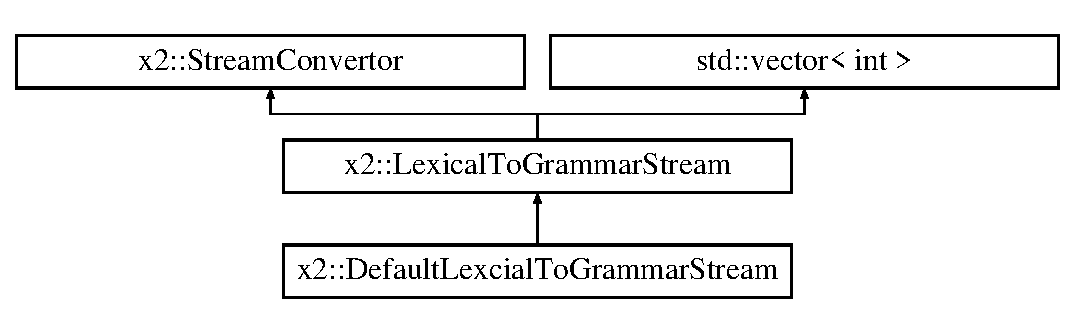
\includegraphics[height=3.000000cm]{classx2_1_1_default_lexcial_to_grammar_stream}
\end{center}
\end{figure}
\subsection*{Public Member Functions}
\begin{DoxyCompactItemize}
\item 
\hyperlink{classx2_1_1_default_lexcial_to_grammar_stream_ab9e8a0468eb091fd118b55ab78adc273}{Default\+Lexcial\+To\+Grammar\+Stream} (const Stream\+Convertor\+::\+Word\+Stream \&wdstream, const \hyperlink{classx2_1_1_gramma}{Gramma} \&g)
\end{DoxyCompactItemize}
\subsection*{Static Public Attributes}
\begin{DoxyCompactItemize}
\item 
static std\+::set$<$ std\+::string $>$ {\bfseries I\+D\+\_\+\+I\+S\+\_\+\+V\+A\+L\+UE}
\end{DoxyCompactItemize}
\subsection*{Additional Inherited Members}


\subsection{Detailed Description}
Lexical\+Parse for c的一个转换流实现器 

\subsection{Constructor \& Destructor Documentation}
\mbox{\Hypertarget{classx2_1_1_default_lexcial_to_grammar_stream_ab9e8a0468eb091fd118b55ab78adc273}\label{classx2_1_1_default_lexcial_to_grammar_stream_ab9e8a0468eb091fd118b55ab78adc273}} 
\index{x2\+::\+Default\+Lexcial\+To\+Grammar\+Stream@{x2\+::\+Default\+Lexcial\+To\+Grammar\+Stream}!Default\+Lexcial\+To\+Grammar\+Stream@{Default\+Lexcial\+To\+Grammar\+Stream}}
\index{Default\+Lexcial\+To\+Grammar\+Stream@{Default\+Lexcial\+To\+Grammar\+Stream}!x2\+::\+Default\+Lexcial\+To\+Grammar\+Stream@{x2\+::\+Default\+Lexcial\+To\+Grammar\+Stream}}
\subsubsection{\texorpdfstring{Default\+Lexcial\+To\+Grammar\+Stream()}{DefaultLexcialToGrammarStream()}}
{\footnotesize\ttfamily x2\+::\+Default\+Lexcial\+To\+Grammar\+Stream\+::\+Default\+Lexcial\+To\+Grammar\+Stream (\begin{DoxyParamCaption}\item[{const Stream\+Convertor\+::\+Word\+Stream \&}]{wdstream,  }\item[{const \hyperlink{classx2_1_1_gramma}{Gramma} \&}]{g }\end{DoxyParamCaption})\hspace{0.3cm}{\ttfamily [inline]}}

抛弃note(注释)

将 T\+Y\+PE=id时,检查内容 为int,返回int 为true/false,返回 

\subsection{Member Data Documentation}
\mbox{\Hypertarget{classx2_1_1_default_lexcial_to_grammar_stream_a007d3e6d792461b8d7693979faa2b4ab}\label{classx2_1_1_default_lexcial_to_grammar_stream_a007d3e6d792461b8d7693979faa2b4ab}} 
\index{x2\+::\+Default\+Lexcial\+To\+Grammar\+Stream@{x2\+::\+Default\+Lexcial\+To\+Grammar\+Stream}!I\+D\+\_\+\+I\+S\+\_\+\+V\+A\+L\+UE@{I\+D\+\_\+\+I\+S\+\_\+\+V\+A\+L\+UE}}
\index{I\+D\+\_\+\+I\+S\+\_\+\+V\+A\+L\+UE@{I\+D\+\_\+\+I\+S\+\_\+\+V\+A\+L\+UE}!x2\+::\+Default\+Lexcial\+To\+Grammar\+Stream@{x2\+::\+Default\+Lexcial\+To\+Grammar\+Stream}}
\subsubsection{\texorpdfstring{I\+D\+\_\+\+I\+S\+\_\+\+V\+A\+L\+UE}{ID\_IS\_VALUE}}
{\footnotesize\ttfamily std\+::set$<$ string $>$ x2\+::\+Default\+Lexcial\+To\+Grammar\+Stream\+::\+I\+D\+\_\+\+I\+S\+\_\+\+V\+A\+L\+UE\hspace{0.3cm}{\ttfamily [static]}}

{\bfseries Initial value\+:}
\begin{DoxyCode}
=\{
                \textcolor{stringliteral}{"int"},
                \textcolor{stringliteral}{"char"},
                \textcolor{stringliteral}{"string"},
                \textcolor{stringliteral}{"return"},
                \textcolor{stringliteral}{"true"},
                \textcolor{stringliteral}{"false"},
        \}
\end{DoxyCode}


The documentation for this class was generated from the following files\+:\begin{DoxyCompactItemize}
\item 
D\+:/\+Pool/eclipse-\/workspace/compiler-\/debug/include/Lexical\+Parser.\+h\item 
D\+:/\+Pool/eclipse-\/workspace/compiler-\/debug/src/Lexical\+Parser.\+cpp\end{DoxyCompactItemize}

\hypertarget{classx2_1_1_default_semantic_action}{}\section{x2\+:\+:Default\+Semantic\+Action Class Reference}
\label{classx2_1_1_default_semantic_action}\index{x2\+::\+Default\+Semantic\+Action@{x2\+::\+Default\+Semantic\+Action}}


根据提议,应当为某些可有可无的适配器提供一个默认实现  




{\ttfamily \#include $<$Grammar\+Translate\+Utils.\+h$>$}

Inheritance diagram for x2\+:\+:Default\+Semantic\+Action\+:\begin{figure}[H]
\begin{center}
\leavevmode
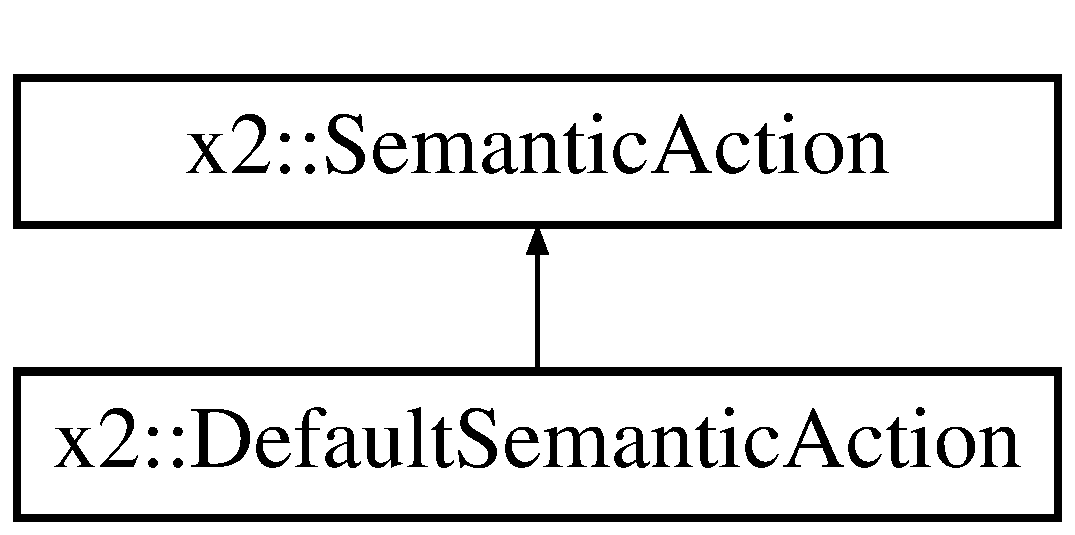
\includegraphics[height=2.000000cm]{classx2_1_1_default_semantic_action}
\end{center}
\end{figure}
\subsection*{Public Member Functions}
\begin{DoxyCompactItemize}
\item 
virtual void \hyperlink{classx2_1_1_default_semantic_action_a25f6cc0ccc04c61ad57bfcf10b9c0cb9}{on\+Reduce} (int i, int j)
\item 
virtual void \hyperlink{classx2_1_1_default_semantic_action_acbd05d5f08396b9df966494bd4422a54}{on\+No\+Goto\+Error} ()
\item 
virtual void \hyperlink{classx2_1_1_default_semantic_action_a6485fcbff1d9b9d63d40112d8887790d}{on\+No\+Action\+Error} ()
\end{DoxyCompactItemize}


\subsection{Detailed Description}
根据提议,应当为某些可有可无的适配器提供一个默认实现 

\subsection{Member Function Documentation}
\mbox{\Hypertarget{classx2_1_1_default_semantic_action_a6485fcbff1d9b9d63d40112d8887790d}\label{classx2_1_1_default_semantic_action_a6485fcbff1d9b9d63d40112d8887790d}} 
\index{x2\+::\+Default\+Semantic\+Action@{x2\+::\+Default\+Semantic\+Action}!on\+No\+Action\+Error@{on\+No\+Action\+Error}}
\index{on\+No\+Action\+Error@{on\+No\+Action\+Error}!x2\+::\+Default\+Semantic\+Action@{x2\+::\+Default\+Semantic\+Action}}
\subsubsection{\texorpdfstring{on\+No\+Action\+Error()}{onNoActionError()}}
{\footnotesize\ttfamily virtual void x2\+::\+Default\+Semantic\+Action\+::on\+No\+Action\+Error (\begin{DoxyParamCaption}{ }\end{DoxyParamCaption})\hspace{0.3cm}{\ttfamily [inline]}, {\ttfamily [virtual]}}

在\+Action\mbox{[}state,a\mbox{]}没有对应的转移的时候调用 

Implements \hyperlink{classx2_1_1_semantic_action_ac8afb7342d18d7d633c234047b16fe27}{x2\+::\+Semantic\+Action}.

\mbox{\Hypertarget{classx2_1_1_default_semantic_action_acbd05d5f08396b9df966494bd4422a54}\label{classx2_1_1_default_semantic_action_acbd05d5f08396b9df966494bd4422a54}} 
\index{x2\+::\+Default\+Semantic\+Action@{x2\+::\+Default\+Semantic\+Action}!on\+No\+Goto\+Error@{on\+No\+Goto\+Error}}
\index{on\+No\+Goto\+Error@{on\+No\+Goto\+Error}!x2\+::\+Default\+Semantic\+Action@{x2\+::\+Default\+Semantic\+Action}}
\subsubsection{\texorpdfstring{on\+No\+Goto\+Error()}{onNoGotoError()}}
{\footnotesize\ttfamily virtual void x2\+::\+Default\+Semantic\+Action\+::on\+No\+Goto\+Error (\begin{DoxyParamCaption}{ }\end{DoxyParamCaption})\hspace{0.3cm}{\ttfamily [inline]}, {\ttfamily [virtual]}}

在\+G\+O\+TO\mbox{[}state,A\mbox{]}没有对应表项的时候调用 

Implements \hyperlink{classx2_1_1_semantic_action_a00d94c579c5962c74ccd5ee6bc9ef70c}{x2\+::\+Semantic\+Action}.

\mbox{\Hypertarget{classx2_1_1_default_semantic_action_a25f6cc0ccc04c61ad57bfcf10b9c0cb9}\label{classx2_1_1_default_semantic_action_a25f6cc0ccc04c61ad57bfcf10b9c0cb9}} 
\index{x2\+::\+Default\+Semantic\+Action@{x2\+::\+Default\+Semantic\+Action}!on\+Reduce@{on\+Reduce}}
\index{on\+Reduce@{on\+Reduce}!x2\+::\+Default\+Semantic\+Action@{x2\+::\+Default\+Semantic\+Action}}
\subsubsection{\texorpdfstring{on\+Reduce()}{onReduce()}}
{\footnotesize\ttfamily virtual void x2\+::\+Default\+Semantic\+Action\+::on\+Reduce (\begin{DoxyParamCaption}\item[{int}]{i,  }\item[{int}]{j }\end{DoxyParamCaption})\hspace{0.3cm}{\ttfamily [inline]}, {\ttfamily [virtual]}}

在产生一个归约式的时候调用. 
\begin{DoxyParams}{Parameters}
{\em i} & \\
\hline
{\em j} & $<$i,j$>$指定使用的产生式,因为它只是个索引,所以你必须知道它所使用的文法实体 \\
\hline
\end{DoxyParams}


Implements \hyperlink{classx2_1_1_semantic_action_a859c5de657a2c684fef66e04a324e980}{x2\+::\+Semantic\+Action}.



The documentation for this class was generated from the following file\+:\begin{DoxyCompactItemize}
\item 
D\+:/\+Pool/eclipse-\/workspace/compiler-\/debug/include/Grammar\+Translate\+Utils.\+h\end{DoxyCompactItemize}

\hypertarget{classx2_1_1_define_preprocessor}{}\section{x2\+:\+:Define\+Preprocessor Class Reference}
\label{classx2_1_1_define_preprocessor}\index{x2\+::\+Define\+Preprocessor@{x2\+::\+Define\+Preprocessor}}
\subsection*{Public Types}
\begin{DoxyCompactItemize}
\item 
\mbox{\Hypertarget{classx2_1_1_define_preprocessor_aeaf9f5de751a2ba570d7e5809a57bf3c}\label{classx2_1_1_define_preprocessor_aeaf9f5de751a2ba570d7e5809a57bf3c}} 
typedef std\+::vector$<$ std\+::string $>$ {\bfseries String\+List}
\item 
\mbox{\Hypertarget{classx2_1_1_define_preprocessor_a15476c94a3988295d4207943d2984783}\label{classx2_1_1_define_preprocessor_a15476c94a3988295d4207943d2984783}} 
typedef std\+::vector$<$ int $>$ {\bfseries Int\+List}
\end{DoxyCompactItemize}
\subsection*{Public Member Functions}
\begin{DoxyCompactItemize}
\item 
\mbox{\Hypertarget{classx2_1_1_define_preprocessor_aa4f8b98ee21103a610aa143c1961da25}\label{classx2_1_1_define_preprocessor_aa4f8b98ee21103a610aa143c1961da25}} 
void {\bfseries init\+With\+Line} (const char $\ast$s, size\+\_\+t \&index, size\+\_\+t len, int \&type)
\item 
\mbox{\Hypertarget{classx2_1_1_define_preprocessor_af5a3f4ee52922f717c429bc8acdbe67a}\label{classx2_1_1_define_preprocessor_af5a3f4ee52922f717c429bc8acdbe67a}} 
void {\bfseries init\+With\+Line} (const std\+::string \&s, size\+\_\+t \&index, int \&type)
\item 
\mbox{\Hypertarget{classx2_1_1_define_preprocessor_ab4f036cfbf86415e805a57d8cca74d08}\label{classx2_1_1_define_preprocessor_ab4f036cfbf86415e805a57d8cca74d08}} 
const String\+List \& {\bfseries get\+Args} () const
\item 
\mbox{\Hypertarget{classx2_1_1_define_preprocessor_ab810660a84df5388d90d385607551c65}\label{classx2_1_1_define_preprocessor_ab810660a84df5388d90d385607551c65}} 
void {\bfseries set\+Args} (const String\+List \&args)
\item 
\mbox{\Hypertarget{classx2_1_1_define_preprocessor_a5713a5bfda359572d01d7c648ef1b415}\label{classx2_1_1_define_preprocessor_a5713a5bfda359572d01d7c648ef1b415}} 
const Int\+List \& {\bfseries get\+Body} () const
\item 
\mbox{\Hypertarget{classx2_1_1_define_preprocessor_a5c709055e64fbf8bc58c2c7f6d66cd3f}\label{classx2_1_1_define_preprocessor_a5c709055e64fbf8bc58c2c7f6d66cd3f}} 
void {\bfseries set\+Body} (const Int\+List \&body)
\item 
\mbox{\Hypertarget{classx2_1_1_define_preprocessor_a7317a9c6b698bc127d25cd2faabb9958}\label{classx2_1_1_define_preprocessor_a7317a9c6b698bc127d25cd2faabb9958}} 
const std\+::string \& {\bfseries get\+Macro\+Name} () const
\item 
\mbox{\Hypertarget{classx2_1_1_define_preprocessor_a66415a4f10cbaf15cf1b33b7e4bf6310}\label{classx2_1_1_define_preprocessor_a66415a4f10cbaf15cf1b33b7e4bf6310}} 
void {\bfseries set\+Macro\+Name} (const std\+::string \&macro\+Name)
\item 
\mbox{\Hypertarget{classx2_1_1_define_preprocessor_a976fcccc95ced64fb7de067f225e3278}\label{classx2_1_1_define_preprocessor_a976fcccc95ced64fb7de067f225e3278}} 
const std\+::string \& {\bfseries get\+Definition} () const
\end{DoxyCompactItemize}
\subsection*{Public Attributes}
\begin{DoxyCompactItemize}
\item 
\mbox{\Hypertarget{classx2_1_1_define_preprocessor_a970d2efccc81da7bb3c4c6e353d920cf}\label{classx2_1_1_define_preprocessor_a970d2efccc81da7bb3c4c6e353d920cf}} 
std\+::string {\bfseries original\+Def}
\item 
\mbox{\Hypertarget{classx2_1_1_define_preprocessor_a6901a2c563b40b5e1a008321a2639c7c}\label{classx2_1_1_define_preprocessor_a6901a2c563b40b5e1a008321a2639c7c}} 
std\+::string {\bfseries macro\+Name}
\item 
\mbox{\Hypertarget{classx2_1_1_define_preprocessor_a8d6aa202f11500f41ad3cadd61f2457d}\label{classx2_1_1_define_preprocessor_a8d6aa202f11500f41ad3cadd61f2457d}} 
String\+List {\bfseries args}
\item 
\mbox{\Hypertarget{classx2_1_1_define_preprocessor_ae4286517adcef6969cafac1bbacbf755}\label{classx2_1_1_define_preprocessor_ae4286517adcef6969cafac1bbacbf755}} 
Int\+List {\bfseries body}
\end{DoxyCompactItemize}


The documentation for this class was generated from the following files\+:\begin{DoxyCompactItemize}
\item 
D\+:/\+Pool/eclipse-\/workspace/compiler-\/debug/include/Lexical\+Parser.\+h\item 
D\+:/\+Pool/eclipse-\/workspace/compiler-\/debug/src/Lexical\+Parser.\+cpp\end{DoxyCompactItemize}

\hypertarget{classx2_1_1_demo_translator}{}\section{x2\+:\+:Demo\+Translator Class Reference}
\label{classx2_1_1_demo_translator}\index{x2\+::\+Demo\+Translator@{x2\+::\+Demo\+Translator}}


A Grammar Translation Demonstrate to Clarify Some Concepts.  




{\ttfamily \#include $<$Grammar\+Translate\+Utils.\+h$>$}

\subsection*{Public Types}
\begin{DoxyCompactItemize}
\item 
\mbox{\Hypertarget{classx2_1_1_demo_translator_a353f41b11b2d282968ddde7f92c8844e}\label{classx2_1_1_demo_translator_a353f41b11b2d282968ddde7f92c8844e}} 
using {\bfseries A\+C\+T\+I\+O\+N\+\_\+\+T\+Y\+PE} = L\+R1\+Gramma\+::\+A\+C\+T\+I\+O\+N\+\_\+\+T\+Y\+PE
\item 
\mbox{\Hypertarget{classx2_1_1_demo_translator_aa08356e09fa72c26524568486fa70b42}\label{classx2_1_1_demo_translator_aa08356e09fa72c26524568486fa70b42}} 
typedef std\+::tuple$<$ int, int, int, int $>$ {\bfseries Quad\+Type}
\item 
\mbox{\Hypertarget{classx2_1_1_demo_translator_a2d71ca79ab44ac76063bc0cedb84fc5e}\label{classx2_1_1_demo_translator_a2d71ca79ab44ac76063bc0cedb84fc5e}} 
typedef std\+::vector$<$ Quad\+Type $>$ {\bfseries Translation\+Type}
\end{DoxyCompactItemize}
\subsection*{Public Member Functions}
\begin{DoxyCompactItemize}
\item 
\hyperlink{classx2_1_1_demo_translator_a5c8a3792ff989f0779f49b4b4824a66d}{Demo\+Translator} (const \hyperlink{classx2_1_1_l_r1_gramma}{L\+R1\+Gramma} \&grammar, const L\+R1\+Gramma\+::\+Info\+Type \&closures\+Info, const \hyperlink{classx2_1_1_gramma_a33681053b045219ea58cc68c3faa4975}{L\+R1\+Gramma\+::\+L\+R\+Analyze\+Table\+Type} \&analyze\+Table, int ending\+Sym, int init\+State=0)
\item 
\mbox{\Hypertarget{classx2_1_1_demo_translator_aa0501ad4afe91afffea6491343c0616c}\label{classx2_1_1_demo_translator_aa0501ad4afe91afffea6491343c0616c}} 
{\bfseries Demo\+Translator} (const \hyperlink{classx2_1_1_demo_translator}{Demo\+Translator} \&t)=default
\item 
\mbox{\Hypertarget{classx2_1_1_demo_translator_a4372d69215029ca5c8fe28489598cfd6}\label{classx2_1_1_demo_translator_a4372d69215029ca5c8fe28489598cfd6}} 
{\bfseries Demo\+Translator} (\hyperlink{classx2_1_1_demo_translator}{Demo\+Translator} \&\&t)=default
\item 
virtual Translation\+Type \hyperlink{classx2_1_1_demo_translator_a5013adbe85fb2bb68d33433454787a02}{translate} (\hyperlink{classx2_1_1_stream_convertor}{Stream\+Convertor} \&input, \hyperlink{classx2_1_1_semantic_action}{Semantic\+Action} \&action) const
\end{DoxyCompactItemize}
\subsection*{Protected Attributes}
\begin{DoxyCompactItemize}
\item 
\mbox{\Hypertarget{classx2_1_1_demo_translator_adbc8cab8e875be2b3bddeb18bfb8eebd}\label{classx2_1_1_demo_translator_adbc8cab8e875be2b3bddeb18bfb8eebd}} 
const \hyperlink{classx2_1_1_l_r1_gramma}{L\+R1\+Gramma} \& {\bfseries grammar}
\item 
\mbox{\Hypertarget{classx2_1_1_demo_translator_a6be6d8958fe9fc1caf0264c9a6a2077f}\label{classx2_1_1_demo_translator_a6be6d8958fe9fc1caf0264c9a6a2077f}} 
const L\+R1\+Gramma\+::\+Info\+Type \& {\bfseries closures\+Info}
\item 
\mbox{\Hypertarget{classx2_1_1_demo_translator_ae1a8138d37f33b2b5662c2327a83c041}\label{classx2_1_1_demo_translator_ae1a8138d37f33b2b5662c2327a83c041}} 
const \hyperlink{classx2_1_1_gramma_a33681053b045219ea58cc68c3faa4975}{Gramma\+::\+L\+R\+Analyze\+Table\+Type} \& {\bfseries analyze\+Table}
\item 
\mbox{\Hypertarget{classx2_1_1_demo_translator_aff2ec433bc4326e419fcbc3c1971badb}\label{classx2_1_1_demo_translator_aff2ec433bc4326e419fcbc3c1971badb}} 
int {\bfseries ending\+Sym}
\item 
\mbox{\Hypertarget{classx2_1_1_demo_translator_a8c1f23b69aab28178a293ded8262a13a}\label{classx2_1_1_demo_translator_a8c1f23b69aab28178a293ded8262a13a}} 
int {\bfseries init\+State}
\end{DoxyCompactItemize}


\subsection{Detailed Description}
A Grammar Translation Demonstrate to Clarify Some Concepts. 

Given a grammar\+: A -\/$>$ T id = E ; A -\/$>$ id = E ; E -\/$>$ ( E ) E -\/$>$ id E -\/$>$ intval E -\/$>$ charval E -\/$>$ E + E E -\/$>$ E $\ast$ E C -\/$>$ A T -\/$>$ int T -\/$>$ char T -\/$>$ string

An Input\+: int a=0; char c=\textquotesingle{}t\textquotesingle{}; a=c; a=d; int a=1;

The Translator should point out that\+:
\begin{DoxyEnumerate}
\item a=c is impossible because their types are not compitable
\item a=d is impossible because d is not defined
\item int a=1 is impossible because a is already defined
\item it should generate a proper code for the right parts
\end{DoxyEnumerate}

自动机构造算法\+: 首先将\+Corrupt\+Table转化为标准的分析表\+Analyze\+Tale类型 初始化\+D\+FA,E\+M\+P\+T\+Y取相同值, failed取\+U\+N\+D\+E\+F\+I\+N\+E\+D值(-\/2), 开始状态为\+I0, 结束状态为为空 遍历\+G\+O\+T\+O表添加变量类型的转移

A\+D\+V\+A\+N\+CE\+: 翻译器是通用的,因此只定义所有翻译器公用的部分. 包括文法引用,分析表引用 语义动作是一个单独的类,指明了某个归约式产生的时候进行某种动作 

\subsection{Constructor \& Destructor Documentation}
\mbox{\Hypertarget{classx2_1_1_demo_translator_a5c8a3792ff989f0779f49b4b4824a66d}\label{classx2_1_1_demo_translator_a5c8a3792ff989f0779f49b4b4824a66d}} 
\index{x2\+::\+Demo\+Translator@{x2\+::\+Demo\+Translator}!Demo\+Translator@{Demo\+Translator}}
\index{Demo\+Translator@{Demo\+Translator}!x2\+::\+Demo\+Translator@{x2\+::\+Demo\+Translator}}
\subsubsection{\texorpdfstring{Demo\+Translator()}{DemoTranslator()}}
{\footnotesize\ttfamily x2\+::\+Demo\+Translator\+::\+Demo\+Translator (\begin{DoxyParamCaption}\item[{const \hyperlink{classx2_1_1_l_r1_gramma}{L\+R1\+Gramma} \&}]{grammar,  }\item[{const L\+R1\+Gramma\+::\+Info\+Type \&}]{closures\+Info,  }\item[{const \hyperlink{classx2_1_1_gramma_a33681053b045219ea58cc68c3faa4975}{L\+R1\+Gramma\+::\+L\+R\+Analyze\+Table\+Type} \&}]{analyze\+Table,  }\item[{int}]{ending\+Sym,  }\item[{int}]{init\+State = {\ttfamily 0} }\end{DoxyParamCaption})\hspace{0.3cm}{\ttfamily [inline]}}


\begin{DoxyParams}{Parameters}
{\em grammar} & 待翻译输入流中使用的文法 \\
\hline
{\em closures\+Info} & 规范集项目族和\+G\+O\+T\+O表,处理方法参见\+L\+R1\+Gramma类的to\+String(info) \\
\hline
{\em analyze\+Table} & 规范的\+L\+R分析表 \\
\hline
{\em ending\+Sym} & 指定结束符号 \$ \\
\hline
{\em init\+State} & 指定这个分析表的起始状态,默认情况下所有的分析表起始状态为0 \\
\hline
\end{DoxyParams}


\subsection{Member Function Documentation}
\mbox{\Hypertarget{classx2_1_1_demo_translator_a5013adbe85fb2bb68d33433454787a02}\label{classx2_1_1_demo_translator_a5013adbe85fb2bb68d33433454787a02}} 
\index{x2\+::\+Demo\+Translator@{x2\+::\+Demo\+Translator}!translate@{translate}}
\index{translate@{translate}!x2\+::\+Demo\+Translator@{x2\+::\+Demo\+Translator}}
\subsubsection{\texorpdfstring{translate()}{translate()}}
{\footnotesize\ttfamily Demo\+Translator\+::\+Translation\+Type x2\+::\+Demo\+Translator\+::translate (\begin{DoxyParamCaption}\item[{\hyperlink{classx2_1_1_stream_convertor}{Stream\+Convertor} \&}]{input,  }\item[{\hyperlink{classx2_1_1_semantic_action}{Semantic\+Action} \&}]{action }\end{DoxyParamCaption}) const\hspace{0.3cm}{\ttfamily [inline]}, {\ttfamily [virtual]}}

在 

The documentation for this class was generated from the following file\+:\begin{DoxyCompactItemize}
\item 
D\+:/\+Pool/eclipse-\/workspace/compiler-\/debug/include/Grammar\+Translate\+Utils.\+h\end{DoxyCompactItemize}

\hypertarget{classx2_1_1_determinastic_f_a}{}\section{x2\+:\+:Determinastic\+FA$<$ T $>$ Class Template Reference}
\label{classx2_1_1_determinastic_f_a}\index{x2\+::\+Determinastic\+F\+A$<$ T $>$@{x2\+::\+Determinastic\+F\+A$<$ T $>$}}


{\ttfamily \#include $<$F\+A\+Utils.\+h$>$}

Inheritance diagram for x2\+:\+:Determinastic\+FA$<$ T $>$\+:\begin{figure}[H]
\begin{center}
\leavevmode
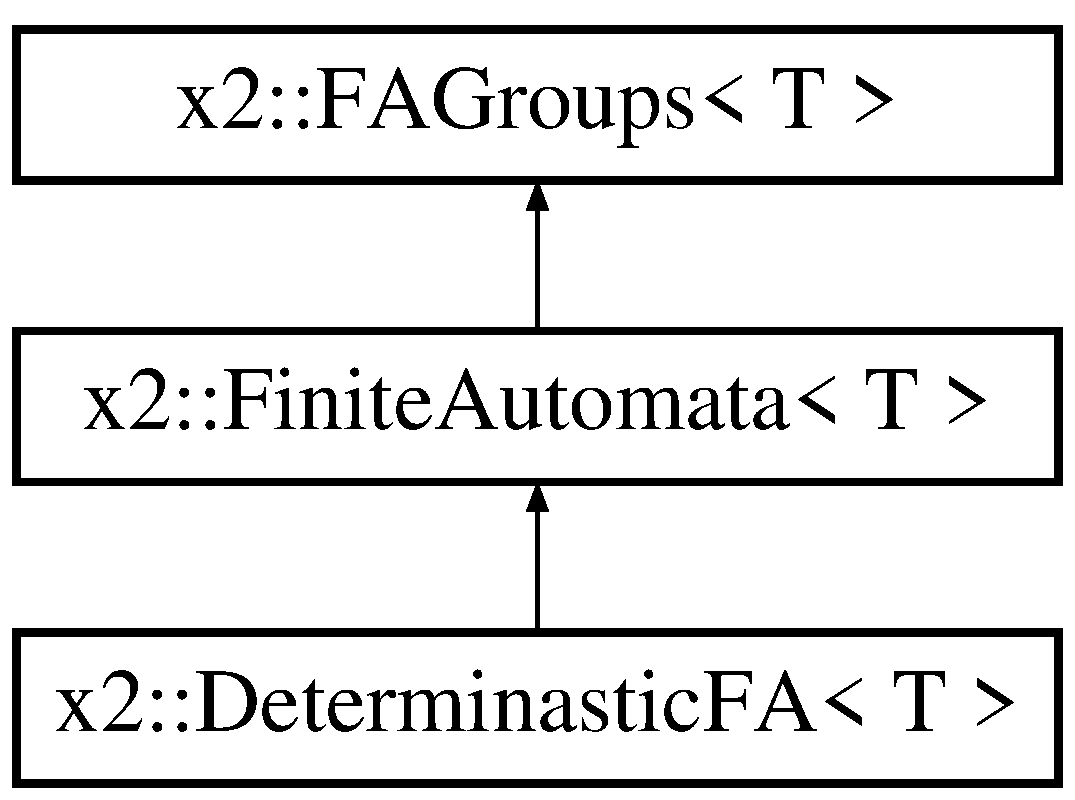
\includegraphics[height=3.000000cm]{classx2_1_1_determinastic_f_a}
\end{center}
\end{figure}
\subsection*{Public Types}
\begin{DoxyCompactItemize}
\item 
\mbox{\Hypertarget{classx2_1_1_determinastic_f_a_a378dc64bebafba6e061dfa0616f73713}\label{classx2_1_1_determinastic_f_a_a378dc64bebafba6e061dfa0616f73713}} 
typedef \hyperlink{classx2_1_1_determinastic_f_a}{Determinastic\+FA}$<$ T $>$ {\bfseries This}
\item 
\mbox{\Hypertarget{classx2_1_1_determinastic_f_a_a6ffacb3640a8d30ec12b6da8435a7026}\label{classx2_1_1_determinastic_f_a_a6ffacb3640a8d30ec12b6da8435a7026}} 
typedef \hyperlink{classx2_1_1_finite_automata}{Finite\+Automata}$<$ T $>$ {\bfseries Father}
\item 
\mbox{\Hypertarget{classx2_1_1_determinastic_f_a_a71618ce7ece8a7d8e969dfba34a71d6a}\label{classx2_1_1_determinastic_f_a_a71618ce7ece8a7d8e969dfba34a71d6a}} 
typedef std\+::vector$<$ T $>$ {\bfseries Input\+Stream\+Type}
\item 
\mbox{\Hypertarget{classx2_1_1_determinastic_f_a_aca059798241ef9f91ec1e613b27790cc}\label{classx2_1_1_determinastic_f_a_aca059798241ef9f91ec1e613b27790cc}} 
typedef std\+::function$<$ void(int, const T \&)$>$ {\bfseries Process\+Fun\+Type}
\end{DoxyCompactItemize}
\subsection*{Public Member Functions}
\begin{DoxyCompactItemize}
\item 
\mbox{\Hypertarget{classx2_1_1_determinastic_f_a_a26fca3362b7a400ba88d7eef9d9cccef}\label{classx2_1_1_determinastic_f_a_a26fca3362b7a400ba88d7eef9d9cccef}} 
{\bfseries Determinastic\+FA} (const T \&emptyT, const T \&failedT, int start\+State, const std\+::vector$<$ int $>$ \&ending\+States)
\item 
\mbox{\Hypertarget{classx2_1_1_determinastic_f_a_a9564061d48e93d38a9de005aaaecb2e4}\label{classx2_1_1_determinastic_f_a_a9564061d48e93d38a9de005aaaecb2e4}} 
{\bfseries Determinastic\+FA} (const T \&emptyT, const T \&failedT, const std\+::string \&start\+State, const std\+::vector$<$ std\+::string $>$ \&ending\+States)
\item 
\mbox{\Hypertarget{classx2_1_1_determinastic_f_a_aa2affbfd0b67bd1a604c015ff4c3764f}\label{classx2_1_1_determinastic_f_a_aa2affbfd0b67bd1a604c015ff4c3764f}} 
{\bfseries Determinastic\+FA} (\hyperlink{classx2_1_1_finite_automata_manager}{Finite\+Automata\+Manager}$<$ T $>$ \&\&faman, int start\+State, const std\+::vector$<$ int $>$ \&ending\+States)
\item 
\mbox{\Hypertarget{classx2_1_1_determinastic_f_a_a3abf4b94adfa0e9d88f48d5db31390d1}\label{classx2_1_1_determinastic_f_a_a3abf4b94adfa0e9d88f48d5db31390d1}} 
{\bfseries Determinastic\+FA} (\hyperlink{classx2_1_1_finite_automata_manager}{Finite\+Automata\+Manager}$<$ T $>$ \&\&faman, const std\+::string \&start\+State, const std\+::vector$<$ std\+::string $>$ \&ending\+States)
\item 
\mbox{\Hypertarget{classx2_1_1_determinastic_f_a_abca31bc4345ac45dd64d5af48c4adf01}\label{classx2_1_1_determinastic_f_a_abca31bc4345ac45dd64d5af48c4adf01}} 
{\bfseries Determinastic\+FA} (const std\+::string \&start\+State, const std\+::vector$<$ std\+::string $>$ \&ending\+States)
\item 
bool \hyperlink{classx2_1_1_determinastic_f_a_a830e6d1612b263d9ef126b29709f4c46}{add\+Transition\+No\+Replace} (int qin, int in, int qout)
\item 
\mbox{\Hypertarget{classx2_1_1_determinastic_f_a_adc6cda2e6a84bacff95f5430c4cbadd6}\label{classx2_1_1_determinastic_f_a_adc6cda2e6a84bacff95f5430c4cbadd6}} 
bool {\bfseries add\+Transition\+No\+Replace} (const std\+::string \&qin, const T \&in, const std\+::string \&qout)
\item 
void \hyperlink{classx2_1_1_determinastic_f_a_a28c9f0dc652f38e8a08d67e2d911d56d}{add\+Transition\+By\+Group} (const std\+::string \&qin, const std\+::string \&group\+Name, const std\+::string \&qout)
\item 
\mbox{\Hypertarget{classx2_1_1_determinastic_f_a_ad373a317b0f3ba584f0ccfab895dff74}\label{classx2_1_1_determinastic_f_a_ad373a317b0f3ba584f0ccfab895dff74}} 
void {\bfseries add\+Transition\+By\+Group} (const std\+::string \&qin, const std\+::set$<$ T $>$ \&group, const std\+::string \&qout)
\item 
void \hyperlink{classx2_1_1_determinastic_f_a_ab5efc90ac528b9d8383b993aa93b6ced}{add\+Transition\+Undefined} (const std\+::string \&qin, const std\+::string \&group\+Base, const std\+::string \&group\+Defined, const std\+::string \&qout)
\item 
\mbox{\Hypertarget{classx2_1_1_determinastic_f_a_aabaaf1756a7628e0652dde5a31e41627}\label{classx2_1_1_determinastic_f_a_aabaaf1756a7628e0652dde5a31e41627}} 
void {\bfseries add\+Transition\+Undefined} (const std\+::string \&qin, const std\+::set$<$ T $>$ \&group\+Base, const std\+::set$<$ T $>$ \&group\+Defined, const std\+::string \&qout)
\item 
\mbox{\Hypertarget{classx2_1_1_determinastic_f_a_a2f71e4692153903869b8200df6b8161d}\label{classx2_1_1_determinastic_f_a_a2f71e4692153903869b8200df6b8161d}} 
void {\bfseries add\+Transition\+Undefined} (const std\+::string \&qin, const std\+::set$<$ T $>$ \&group\+Base, const std\+::string \&group\+Defined, const std\+::string \&qout)
\item 
void \hyperlink{classx2_1_1_determinastic_f_a_adbd0f99ea29d31abd9f9675ee5b9fdef}{add\+Transition} (int qin, int in, int qout)
\item 
\mbox{\Hypertarget{classx2_1_1_determinastic_f_a_a64c85bde0d8df31c30758cfcb1acaf2c}\label{classx2_1_1_determinastic_f_a_a64c85bde0d8df31c30758cfcb1acaf2c}} 
void {\bfseries add\+Transition} (const std\+::string \&qin, const T \&in, const std\+::string \&qout)
\item 
\mbox{\Hypertarget{classx2_1_1_determinastic_f_a_a2dce2abc6c295032900475c6d3a2bfcf}\label{classx2_1_1_determinastic_f_a_a2dce2abc6c295032900475c6d3a2bfcf}} 
void {\bfseries add\+Goback} (int qin, int qout)
\item 
\mbox{\Hypertarget{classx2_1_1_determinastic_f_a_a63cba8c5c4df112ab140d1d8c674635b}\label{classx2_1_1_determinastic_f_a_a63cba8c5c4df112ab140d1d8c674635b}} 
void {\bfseries add\+Goback} (const std\+::string \&qin, const std\+::string \&qout)
\item 
\mbox{\Hypertarget{classx2_1_1_determinastic_f_a_a3761a086c847df17777820e80dae2470}\label{classx2_1_1_determinastic_f_a_a3761a086c847df17777820e80dae2470}} 
void {\bfseries add\+Goback} (const std\+::initializer\+\_\+list$<$ std\+::pair$<$ std\+::string, std\+::string $>$$>$ list)
\item 
\mbox{\Hypertarget{classx2_1_1_determinastic_f_a_a0253fbb1048b2ff90dc79b9d9379be96}\label{classx2_1_1_determinastic_f_a_a0253fbb1048b2ff90dc79b9d9379be96}} 
void {\bfseries add\+Goback} (const std\+::vector$<$ std\+::pair$<$ std\+::string, std\+::string $>$$>$ list)
\item 
\mbox{\Hypertarget{classx2_1_1_determinastic_f_a_ab25d920d2d20793dda5c507d9a109649}\label{classx2_1_1_determinastic_f_a_ab25d920d2d20793dda5c507d9a109649}} 
void {\bfseries add\+Stop} (int q)
\item 
\mbox{\Hypertarget{classx2_1_1_determinastic_f_a_a619dbc83e0a3e33e8fd8f9199f827011}\label{classx2_1_1_determinastic_f_a_a619dbc83e0a3e33e8fd8f9199f827011}} 
void {\bfseries add\+Stop} (std\+::initializer\+\_\+list$<$ int $>$ list)
\item 
\mbox{\Hypertarget{classx2_1_1_determinastic_f_a_ab6979f20952c95845a5fc55c5cd71ab3}\label{classx2_1_1_determinastic_f_a_ab6979f20952c95845a5fc55c5cd71ab3}} 
void {\bfseries add\+Stop} (const std\+::string \&q)
\item 
\mbox{\Hypertarget{classx2_1_1_determinastic_f_a_ad25513f1d72fd086db1f4dba68ac632b}\label{classx2_1_1_determinastic_f_a_ad25513f1d72fd086db1f4dba68ac632b}} 
void {\bfseries add\+Stop} (std\+::initializer\+\_\+list$<$ std\+::string $>$ list)
\item 
bool \hyperlink{classx2_1_1_determinastic_f_a_afd31af3cc87e3d372900fa62da926a69}{next} (const T \&in)
\item 
\mbox{\Hypertarget{classx2_1_1_determinastic_f_a_acfec740ee6f94dfe4d522dc2224047bd}\label{classx2_1_1_determinastic_f_a_acfec740ee6f94dfe4d522dc2224047bd}} 
bool {\bfseries next} (int in)
\item 
\mbox{\Hypertarget{classx2_1_1_determinastic_f_a_a3d453ac8a55453c3f87d1cb040924497}\label{classx2_1_1_determinastic_f_a_a3d453ac8a55453c3f87d1cb040924497}} 
virtual void {\bfseries get\+Match} (const Input\+Stream\+Type \&instream, \hyperlink{classx2_1_1_output_stream_processor}{Output\+Stream\+Processor}$<$ T $>$ \&outstream)
\item 
\mbox{\Hypertarget{classx2_1_1_determinastic_f_a_a0f2257b373cedc43e09b187650d0b949}\label{classx2_1_1_determinastic_f_a_a0f2257b373cedc43e09b187650d0b949}} 
virtual void {\bfseries get\+Match} (const Input\+Stream\+Type \&instream, Process\+Fun\+Type process)
\item 
\mbox{\Hypertarget{classx2_1_1_determinastic_f_a_a60140cc24c0cc9369dd485cbcb550717}\label{classx2_1_1_determinastic_f_a_a60140cc24c0cc9369dd485cbcb550717}} 
std\+::string {\bfseries to\+String} () const
\end{DoxyCompactItemize}
\subsection*{Protected Attributes}
\begin{DoxyCompactItemize}
\item 
\mbox{\Hypertarget{classx2_1_1_determinastic_f_a_af9b7f7a6ed38d7611e1cb8c774617167}\label{classx2_1_1_determinastic_f_a_af9b7f7a6ed38d7611e1cb8c774617167}} 
std\+::map$<$ std\+::pair$<$ int, int $>$, int $>$ {\bfseries transitions}
\item 
\mbox{\Hypertarget{classx2_1_1_determinastic_f_a_a2a7e3e6089bb8873125bb2983ff90ea7}\label{classx2_1_1_determinastic_f_a_a2a7e3e6089bb8873125bb2983ff90ea7}} 
std\+::set$<$ std\+::pair$<$ int, int $>$ $>$ {\bfseries gobacks}
\item 
\mbox{\Hypertarget{classx2_1_1_determinastic_f_a_abcb3e36327c33dde71139e8156734149}\label{classx2_1_1_determinastic_f_a_abcb3e36327c33dde71139e8156734149}} 
std\+::set$<$ int $>$ {\bfseries stops}
\end{DoxyCompactItemize}
\subsection*{Additional Inherited Members}


\subsection{Detailed Description}
\subsubsection*{template$<$class T$>$\newline
class x2\+::\+Determinastic\+F\+A$<$ T $>$}

FA that can generate output stream.

软约束: 对已经添加过的产生式不修改 

\subsection{Member Function Documentation}
\mbox{\Hypertarget{classx2_1_1_determinastic_f_a_adbd0f99ea29d31abd9f9675ee5b9fdef}\label{classx2_1_1_determinastic_f_a_adbd0f99ea29d31abd9f9675ee5b9fdef}} 
\index{x2\+::\+Determinastic\+FA@{x2\+::\+Determinastic\+FA}!add\+Transition@{add\+Transition}}
\index{add\+Transition@{add\+Transition}!x2\+::\+Determinastic\+FA@{x2\+::\+Determinastic\+FA}}
\subsubsection{\texorpdfstring{add\+Transition()}{addTransition()}}
{\footnotesize\ttfamily template$<$class T $>$ \\
void \hyperlink{classx2_1_1_determinastic_f_a}{x2\+::\+Determinastic\+FA}$<$ T $>$\+::add\+Transition (\begin{DoxyParamCaption}\item[{int}]{qin,  }\item[{int}]{in,  }\item[{int}]{qout }\end{DoxyParamCaption})\hspace{0.3cm}{\ttfamily [virtual]}}

default is add-\/replace 

Implements \hyperlink{classx2_1_1_finite_automata_ac8f011bb86cb9e47370274ae200fc769}{x2\+::\+Finite\+Automata$<$ T $>$}.

\mbox{\Hypertarget{classx2_1_1_determinastic_f_a_a28c9f0dc652f38e8a08d67e2d911d56d}\label{classx2_1_1_determinastic_f_a_a28c9f0dc652f38e8a08d67e2d911d56d}} 
\index{x2\+::\+Determinastic\+FA@{x2\+::\+Determinastic\+FA}!add\+Transition\+By\+Group@{add\+Transition\+By\+Group}}
\index{add\+Transition\+By\+Group@{add\+Transition\+By\+Group}!x2\+::\+Determinastic\+FA@{x2\+::\+Determinastic\+FA}}
\subsubsection{\texorpdfstring{add\+Transition\+By\+Group()}{addTransitionByGroup()}}
{\footnotesize\ttfamily template$<$class T $>$ \\
void \hyperlink{classx2_1_1_determinastic_f_a}{x2\+::\+Determinastic\+FA}$<$ T $>$\+::add\+Transition\+By\+Group (\begin{DoxyParamCaption}\item[{const std\+::string \&}]{qin,  }\item[{const std\+::string \&}]{group\+Name,  }\item[{const std\+::string \&}]{qout }\end{DoxyParamCaption})\hspace{0.3cm}{\ttfamily [inline]}}

the group operation will not overload the single defined transition

if a symbol in a group is not in the symbol list, it will be added. \mbox{\Hypertarget{classx2_1_1_determinastic_f_a_a830e6d1612b263d9ef126b29709f4c46}\label{classx2_1_1_determinastic_f_a_a830e6d1612b263d9ef126b29709f4c46}} 
\index{x2\+::\+Determinastic\+FA@{x2\+::\+Determinastic\+FA}!add\+Transition\+No\+Replace@{add\+Transition\+No\+Replace}}
\index{add\+Transition\+No\+Replace@{add\+Transition\+No\+Replace}!x2\+::\+Determinastic\+FA@{x2\+::\+Determinastic\+FA}}
\subsubsection{\texorpdfstring{add\+Transition\+No\+Replace()}{addTransitionNoReplace()}}
{\footnotesize\ttfamily template$<$class T $>$ \\
bool \hyperlink{classx2_1_1_determinastic_f_a}{x2\+::\+Determinastic\+FA}$<$ T $>$\+::add\+Transition\+No\+Replace (\begin{DoxyParamCaption}\item[{int}]{qin,  }\item[{int}]{in,  }\item[{int}]{qout }\end{DoxyParamCaption})}

if non-\/exist,add it,else return failed. \mbox{\Hypertarget{classx2_1_1_determinastic_f_a_ab5efc90ac528b9d8383b993aa93b6ced}\label{classx2_1_1_determinastic_f_a_ab5efc90ac528b9d8383b993aa93b6ced}} 
\index{x2\+::\+Determinastic\+FA@{x2\+::\+Determinastic\+FA}!add\+Transition\+Undefined@{add\+Transition\+Undefined}}
\index{add\+Transition\+Undefined@{add\+Transition\+Undefined}!x2\+::\+Determinastic\+FA@{x2\+::\+Determinastic\+FA}}
\subsubsection{\texorpdfstring{add\+Transition\+Undefined()}{addTransitionUndefined()}}
{\footnotesize\ttfamily template$<$class T $>$ \\
void \hyperlink{classx2_1_1_determinastic_f_a}{x2\+::\+Determinastic\+FA}$<$ T $>$\+::add\+Transition\+Undefined (\begin{DoxyParamCaption}\item[{const std\+::string \&}]{qin,  }\item[{const std\+::string \&}]{group\+Base,  }\item[{const std\+::string \&}]{group\+Defined,  }\item[{const std\+::string \&}]{qout }\end{DoxyParamCaption})\hspace{0.3cm}{\ttfamily [inline]}}

add g\+Base -\/ g\+Defined \mbox{\Hypertarget{classx2_1_1_determinastic_f_a_afd31af3cc87e3d372900fa62da926a69}\label{classx2_1_1_determinastic_f_a_afd31af3cc87e3d372900fa62da926a69}} 
\index{x2\+::\+Determinastic\+FA@{x2\+::\+Determinastic\+FA}!next@{next}}
\index{next@{next}!x2\+::\+Determinastic\+FA@{x2\+::\+Determinastic\+FA}}
\subsubsection{\texorpdfstring{next()}{next()}}
{\footnotesize\ttfamily template$<$class T $>$ \\
bool \hyperlink{classx2_1_1_determinastic_f_a}{x2\+::\+Determinastic\+FA}$<$ T $>$\+::next (\begin{DoxyParamCaption}\item[{const T \&}]{in }\end{DoxyParamCaption})\hspace{0.3cm}{\ttfamily [inline]}}

goto next state on input in,if failed return failed,else return succeed. 

The documentation for this class was generated from the following file\+:\begin{DoxyCompactItemize}
\item 
D\+:/\+Pool/eclipse-\/workspace/compiler-\/debug/include/F\+A\+Utils.\+h\end{DoxyCompactItemize}

\hypertarget{classx2_1_1_f_a_groups}{}\section{x2\+:\+:F\+A\+Groups$<$ T $>$ Class Template Reference}
\label{classx2_1_1_f_a_groups}\index{x2\+::\+F\+A\+Groups$<$ T $>$@{x2\+::\+F\+A\+Groups$<$ T $>$}}


{\ttfamily \#include $<$F\+A\+Utils.\+h$>$}

Inheritance diagram for x2\+:\+:F\+A\+Groups$<$ T $>$\+:\begin{figure}[H]
\begin{center}
\leavevmode
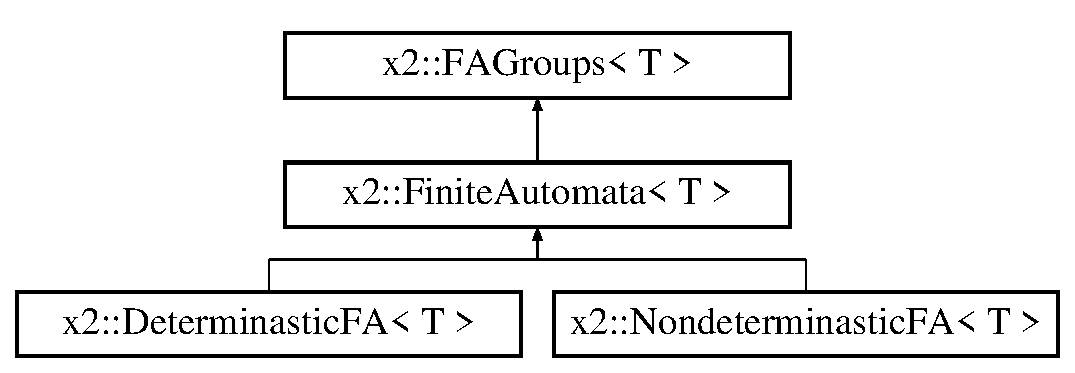
\includegraphics[height=3.000000cm]{classx2_1_1_f_a_groups}
\end{center}
\end{figure}
\subsection*{Public Member Functions}
\begin{DoxyCompactItemize}
\item 
\mbox{\Hypertarget{classx2_1_1_f_a_groups_a0c6b1e7746fd561a386655d972e80b6c}\label{classx2_1_1_f_a_groups_a0c6b1e7746fd561a386655d972e80b6c}} 
bool {\bfseries add\+Group} (const std\+::string \&name, const std\+::set$<$ T $>$ \&group)
\item 
\mbox{\Hypertarget{classx2_1_1_f_a_groups_a3d84f81aa2a8f1e3c070e2e7e564b638}\label{classx2_1_1_f_a_groups_a3d84f81aa2a8f1e3c070e2e7e564b638}} 
bool {\bfseries add\+Group} (const std\+::string \&name, std\+::set$<$ T $>$ \&\&group)
\item 
\mbox{\Hypertarget{classx2_1_1_f_a_groups_a23f88d7b2340e3135b2d3c66d8c330f5}\label{classx2_1_1_f_a_groups_a23f88d7b2340e3135b2d3c66d8c330f5}} 
bool {\bfseries in\+Group} (const T \&t, const std\+::string \&name) const
\item 
\mbox{\Hypertarget{classx2_1_1_f_a_groups_ac71065a983c8e48c47065769214b2da6}\label{classx2_1_1_f_a_groups_ac71065a983c8e48c47065769214b2da6}} 
bool {\bfseries has\+Group} (const std\+::string \&name) const
\item 
\mbox{\Hypertarget{classx2_1_1_f_a_groups_a36d6e1c69dfa5f5dad26d3e9243807e9}\label{classx2_1_1_f_a_groups_a36d6e1c69dfa5f5dad26d3e9243807e9}} 
const std\+::set$<$ T $>$ \& {\bfseries get\+Group} (const std\+::string \&name) const
\item 
\mbox{\Hypertarget{classx2_1_1_f_a_groups_a7bbfea3b525be2c654251497eeaa76bb}\label{classx2_1_1_f_a_groups_a7bbfea3b525be2c654251497eeaa76bb}} 
bool {\bfseries is\+Group\+Undefined} (const std\+::string \&group) const
\item 
\mbox{\Hypertarget{classx2_1_1_f_a_groups_a50f9de5cd5023c9b6320ad5dd1a03a22}\label{classx2_1_1_f_a_groups_a50f9de5cd5023c9b6320ad5dd1a03a22}} 
bool {\bfseries is\+Group\+Undefined} (const std\+::set$<$ T $>$ \&group) const
\item 
\mbox{\Hypertarget{classx2_1_1_f_a_groups_af9d56e53d92a1e11b0a2bf1a9991bbe5}\label{classx2_1_1_f_a_groups_af9d56e53d92a1e11b0a2bf1a9991bbe5}} 
bool {\bfseries add\+Group\+Union} (const std\+::string \&new\+Group, const std\+::vector$<$ std\+::string $>$ groups)
\item 
\mbox{\Hypertarget{classx2_1_1_f_a_groups_a2a398b4a8151c3c54b6db40dfb8298ee}\label{classx2_1_1_f_a_groups_a2a398b4a8151c3c54b6db40dfb8298ee}} 
bool {\bfseries add\+Group\+Diff} (const std\+::string \&new\+Group, const std\+::string \&group\+Base, const std\+::string \&group\+Defined)
\item 
\mbox{\Hypertarget{classx2_1_1_f_a_groups_a37bfd53df1493cb777387d8f09aaf112}\label{classx2_1_1_f_a_groups_a37bfd53df1493cb777387d8f09aaf112}} 
bool {\bfseries add\+Group\+Union} (const std\+::string \&new\+Group, const std\+::string \&groups1, const std\+::set$<$ T $>$ \&group\+Outter)
\end{DoxyCompactItemize}
\subsection*{Protected Attributes}
\begin{DoxyCompactItemize}
\item 
\mbox{\Hypertarget{classx2_1_1_f_a_groups_a5c5e18182fce69e70ed81937bbcae877}\label{classx2_1_1_f_a_groups_a5c5e18182fce69e70ed81937bbcae877}} 
std\+::map$<$ std\+::string, std\+::set$<$ T $>$ $>$ {\bfseries groups}
\end{DoxyCompactItemize}
\subsection*{Static Protected Attributes}
\begin{DoxyCompactItemize}
\item 
\mbox{\Hypertarget{classx2_1_1_f_a_groups_a9836c66d59da2c3d1e25811b608f6cc9}\label{classx2_1_1_f_a_groups_a9836c66d59da2c3d1e25811b608f6cc9}} 
static const std\+::set$<$ T $>$ {\bfseries U\+N\+D\+E\+F\+I\+N\+E\+D\+\_\+\+G\+R\+O\+UP} = std\+::set$<$T$>$()
\end{DoxyCompactItemize}


\subsection{Detailed Description}
\subsubsection*{template$<$class T$>$\newline
class x2\+::\+F\+A\+Groups$<$ T $>$}

T as group element type 

The documentation for this class was generated from the following file\+:\begin{DoxyCompactItemize}
\item 
D\+:/\+Pool/eclipse-\/workspace/compiler-\/debug/include/F\+A\+Utils.\+h\end{DoxyCompactItemize}

\hypertarget{classx2_1_1_finite_automata}{}\section{x2\+:\+:Finite\+Automata$<$ T $>$ Class Template Reference}
\label{classx2_1_1_finite_automata}\index{x2\+::\+Finite\+Automata$<$ T $>$@{x2\+::\+Finite\+Automata$<$ T $>$}}


{\ttfamily \#include $<$F\+A\+Utils.\+h$>$}

Inheritance diagram for x2\+:\+:Finite\+Automata$<$ T $>$\+:\begin{figure}[H]
\begin{center}
\leavevmode
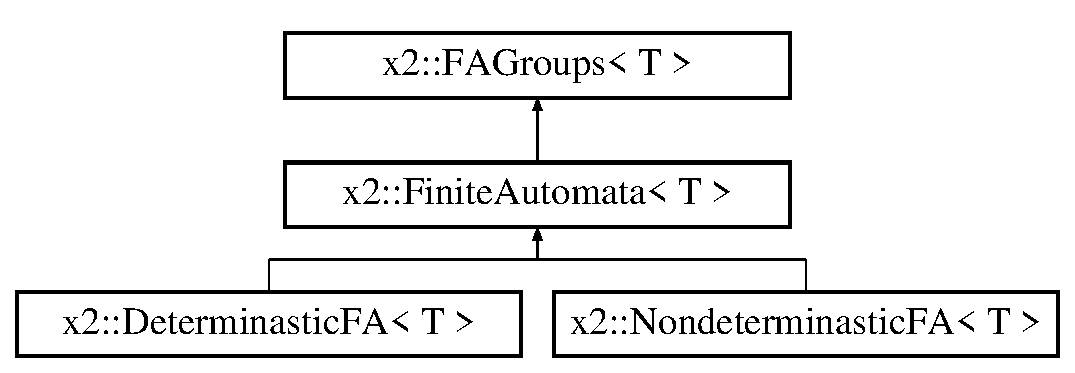
\includegraphics[height=3.000000cm]{classx2_1_1_finite_automata}
\end{center}
\end{figure}
\subsection*{Public Types}
\begin{DoxyCompactItemize}
\item 
\mbox{\Hypertarget{classx2_1_1_finite_automata_a1e633b48bb19ff2de32c037f305eb084}\label{classx2_1_1_finite_automata_a1e633b48bb19ff2de32c037f305eb084}} 
typedef std\+::vector$<$ T $>$ {\bfseries Input\+Stream\+Type}
\item 
\mbox{\Hypertarget{classx2_1_1_finite_automata_a31301b2b4958a62b3565e41c23eca2e4}\label{classx2_1_1_finite_automata_a31301b2b4958a62b3565e41c23eca2e4}} 
typedef \hyperlink{classx2_1_1_finite_automata}{Finite\+Automata}$<$ T $>$ {\bfseries This}
\item 
\mbox{\Hypertarget{classx2_1_1_finite_automata_ab8b9e1d69f545925a2d0ae7b6d91bdc4}\label{classx2_1_1_finite_automata_ab8b9e1d69f545925a2d0ae7b6d91bdc4}} 
typedef std\+::function$<$ void(int, const T \&)$>$ {\bfseries Process\+Fun\+Type}
\end{DoxyCompactItemize}
\subsection*{Public Member Functions}
\begin{DoxyCompactItemize}
\item 
\mbox{\Hypertarget{classx2_1_1_finite_automata_a7ab5a598af5fe719caccb661c71829d6}\label{classx2_1_1_finite_automata_a7ab5a598af5fe719caccb661c71829d6}} 
{\bfseries Finite\+Automata} (const T \&emptyT, const T \&failedT, int start\+State, const std\+::vector$<$ int $>$ \&ending\+States)
\item 
\mbox{\Hypertarget{classx2_1_1_finite_automata_a1a9802db45527e15f561af9b6e8c8af7}\label{classx2_1_1_finite_automata_a1a9802db45527e15f561af9b6e8c8af7}} 
{\bfseries Finite\+Automata} (const T \&emptyT, const T \&failedT, const std\+::string \&start\+State, const std\+::vector$<$ std\+::string $>$ \&ending\+States)
\item 
\mbox{\Hypertarget{classx2_1_1_finite_automata_aace90dedecd2d57a9a058801c608aa9a}\label{classx2_1_1_finite_automata_aace90dedecd2d57a9a058801c608aa9a}} 
{\bfseries Finite\+Automata} (\hyperlink{classx2_1_1_finite_automata_manager}{Finite\+Automata\+Manager}$<$ T $>$ \&\&faman, int start\+State, const std\+::vector$<$ int $>$ \&ending\+States)
\item 
\mbox{\Hypertarget{classx2_1_1_finite_automata_a3a32bbd929198b40ad1a829cb5e1677c}\label{classx2_1_1_finite_automata_a3a32bbd929198b40ad1a829cb5e1677c}} 
{\bfseries Finite\+Automata} (\hyperlink{classx2_1_1_finite_automata_manager}{Finite\+Automata\+Manager}$<$ T $>$ \&\&faman, const std\+::string \&start\+State, const std\+::vector$<$ std\+::string $>$ \&ending\+States)
\item 
\mbox{\Hypertarget{classx2_1_1_finite_automata_a1c7905401495f3496476c49ba2a22760}\label{classx2_1_1_finite_automata_a1c7905401495f3496476c49ba2a22760}} 
const std\+::string \& {\bfseries get\+Current\+State} () const
\item 
\mbox{\Hypertarget{classx2_1_1_finite_automata_a23c483414a3639840cf6697615852512}\label{classx2_1_1_finite_automata_a23c483414a3639840cf6697615852512}} 
int {\bfseries query\+State} (const std\+::string \&state) const
\item 
\mbox{\Hypertarget{classx2_1_1_finite_automata_a85ff5c6205df2affc904cce0765050a7}\label{classx2_1_1_finite_automata_a85ff5c6205df2affc904cce0765050a7}} 
int {\bfseries query\+Symbol} (const T \&t) const
\item 
int \hyperlink{classx2_1_1_finite_automata_a44ca86f1589eeaa77ab73f953033c5a5}{query\+State\+Add} (const std\+::string \&state)
\item 
\mbox{\Hypertarget{classx2_1_1_finite_automata_a36bd258d031bea1d3e31dbc674047c51}\label{classx2_1_1_finite_automata_a36bd258d031bea1d3e31dbc674047c51}} 
int {\bfseries query\+Symbol\+Add} (const T \&t)
\item 
\mbox{\Hypertarget{classx2_1_1_finite_automata_a96ed2d1841cde70fb1d7d51a62fbb2e4}\label{classx2_1_1_finite_automata_a96ed2d1841cde70fb1d7d51a62fbb2e4}} 
const std\+::string \& {\bfseries query\+State} (int state) const
\item 
\mbox{\Hypertarget{classx2_1_1_finite_automata_a2fb9ac68cd1c068b1ccb56d54ba04181}\label{classx2_1_1_finite_automata_a2fb9ac68cd1c068b1ccb56d54ba04181}} 
const T \& {\bfseries query\+Symbol} (int sym) const
\item 
void \hyperlink{classx2_1_1_finite_automata_ab645c9a82ae95bda44e60dce1568bcad}{reset} ()
\item 
bool \hyperlink{classx2_1_1_finite_automata_a993fb22633638494c8a267cd2c5329fc}{at\+End} () const
\item 
virtual void \hyperlink{classx2_1_1_finite_automata_ac8f011bb86cb9e47370274ae200fc769}{add\+Transition} (int qin, int in, int qout)=0
\item 
\mbox{\Hypertarget{classx2_1_1_finite_automata_a0a6920e26afbb6ec5f3ead1803cf132a}\label{classx2_1_1_finite_automata_a0a6920e26afbb6ec5f3ead1803cf132a}} 
virtual void {\bfseries get\+Match} (const Input\+Stream\+Type \&instream, \hyperlink{classx2_1_1_output_stream_processor}{Output\+Stream\+Processor}$<$ T $>$ \&outstream)=0
\item 
\mbox{\Hypertarget{classx2_1_1_finite_automata_a0cdcee5c903196276d63e6befd3608f5}\label{classx2_1_1_finite_automata_a0cdcee5c903196276d63e6befd3608f5}} 
virtual void {\bfseries get\+Match} (const Input\+Stream\+Type \&instream, Process\+Fun\+Type process)=0
\item 
\mbox{\Hypertarget{classx2_1_1_finite_automata_a08657406175592e9312e6f6a7609b14d}\label{classx2_1_1_finite_automata_a08657406175592e9312e6f6a7609b14d}} 
std\+::string {\bfseries to\+String} () const
\end{DoxyCompactItemize}
\subsection*{Protected Attributes}
\begin{DoxyCompactItemize}
\item 
\mbox{\Hypertarget{classx2_1_1_finite_automata_a260a676437a198ee7d0c9a3881ac6089}\label{classx2_1_1_finite_automata_a260a676437a198ee7d0c9a3881ac6089}} 
\hyperlink{classx2_1_1_finite_automata_manager}{Finite\+Automata\+Manager}$<$ T $>$ {\bfseries F\+Aman}
\item 
\mbox{\Hypertarget{classx2_1_1_finite_automata_a682403e099f477d982734253cda1fb4d}\label{classx2_1_1_finite_automata_a682403e099f477d982734253cda1fb4d}} 
int {\bfseries start\+State}
\item 
\mbox{\Hypertarget{classx2_1_1_finite_automata_a5d56c81d319e70709c46dad540ce5ae7}\label{classx2_1_1_finite_automata_a5d56c81d319e70709c46dad540ce5ae7}} 
std\+::set$<$ int $>$ {\bfseries ending\+States}
\item 
\mbox{\Hypertarget{classx2_1_1_finite_automata_a36073aa55410869390e8276ce6e5ebd5}\label{classx2_1_1_finite_automata_a36073aa55410869390e8276ce6e5ebd5}} 
int {\bfseries cur\+State}
\end{DoxyCompactItemize}
\subsection*{Additional Inherited Members}


\subsection{Detailed Description}
\subsubsection*{template$<$class T$>$\newline
class x2\+::\+Finite\+Automata$<$ T $>$}

输入流既可以是 vector,也可以是string;

如果输入流是int,需要另外处理

\+: in C++ does not mean extending, it means that it has such part 

\subsection{Member Function Documentation}
\mbox{\Hypertarget{classx2_1_1_finite_automata_ac8f011bb86cb9e47370274ae200fc769}\label{classx2_1_1_finite_automata_ac8f011bb86cb9e47370274ae200fc769}} 
\index{x2\+::\+Finite\+Automata@{x2\+::\+Finite\+Automata}!add\+Transition@{add\+Transition}}
\index{add\+Transition@{add\+Transition}!x2\+::\+Finite\+Automata@{x2\+::\+Finite\+Automata}}
\subsubsection{\texorpdfstring{add\+Transition()}{addTransition()}}
{\footnotesize\ttfamily template$<$class T$>$ \\
virtual void \hyperlink{classx2_1_1_finite_automata}{x2\+::\+Finite\+Automata}$<$ T $>$\+::add\+Transition (\begin{DoxyParamCaption}\item[{int}]{qin,  }\item[{int}]{in,  }\item[{int}]{qout }\end{DoxyParamCaption})\hspace{0.3cm}{\ttfamily [pure virtual]}}

default is add-\/replace 

Implemented in \hyperlink{classx2_1_1_determinastic_f_a_adbd0f99ea29d31abd9f9675ee5b9fdef}{x2\+::\+Determinastic\+F\+A$<$ T $>$}.

\mbox{\Hypertarget{classx2_1_1_finite_automata_a993fb22633638494c8a267cd2c5329fc}\label{classx2_1_1_finite_automata_a993fb22633638494c8a267cd2c5329fc}} 
\index{x2\+::\+Finite\+Automata@{x2\+::\+Finite\+Automata}!at\+End@{at\+End}}
\index{at\+End@{at\+End}!x2\+::\+Finite\+Automata@{x2\+::\+Finite\+Automata}}
\subsubsection{\texorpdfstring{at\+End()}{atEnd()}}
{\footnotesize\ttfamily template$<$class T $>$ \\
bool \hyperlink{classx2_1_1_finite_automata}{x2\+::\+Finite\+Automata}$<$ T $>$\+::at\+End (\begin{DoxyParamCaption}{ }\end{DoxyParamCaption}) const\hspace{0.3cm}{\ttfamily [inline]}}

if current state is accepted \mbox{\Hypertarget{classx2_1_1_finite_automata_a44ca86f1589eeaa77ab73f953033c5a5}\label{classx2_1_1_finite_automata_a44ca86f1589eeaa77ab73f953033c5a5}} 
\index{x2\+::\+Finite\+Automata@{x2\+::\+Finite\+Automata}!query\+State\+Add@{query\+State\+Add}}
\index{query\+State\+Add@{query\+State\+Add}!x2\+::\+Finite\+Automata@{x2\+::\+Finite\+Automata}}
\subsubsection{\texorpdfstring{query\+State\+Add()}{queryStateAdd()}}
{\footnotesize\ttfamily template$<$class T $>$ \\
int \hyperlink{classx2_1_1_finite_automata}{x2\+::\+Finite\+Automata}$<$ T $>$\+::query\+State\+Add (\begin{DoxyParamCaption}\item[{const std\+::string \&}]{state }\end{DoxyParamCaption})\hspace{0.3cm}{\ttfamily [inline]}}

if non-\/exist, add it and return \mbox{\Hypertarget{classx2_1_1_finite_automata_ab645c9a82ae95bda44e60dce1568bcad}\label{classx2_1_1_finite_automata_ab645c9a82ae95bda44e60dce1568bcad}} 
\index{x2\+::\+Finite\+Automata@{x2\+::\+Finite\+Automata}!reset@{reset}}
\index{reset@{reset}!x2\+::\+Finite\+Automata@{x2\+::\+Finite\+Automata}}
\subsubsection{\texorpdfstring{reset()}{reset()}}
{\footnotesize\ttfamily template$<$class T $>$ \\
void \hyperlink{classx2_1_1_finite_automata}{x2\+::\+Finite\+Automata}$<$ T $>$\+::reset (\begin{DoxyParamCaption}{ }\end{DoxyParamCaption})\hspace{0.3cm}{\ttfamily [inline]}}

reset all state-\/related information, restart at start\+State 

The documentation for this class was generated from the following file\+:\begin{DoxyCompactItemize}
\item 
D\+:/\+Pool/eclipse-\/workspace/compiler-\/debug/include/F\+A\+Utils.\+h\end{DoxyCompactItemize}

\hypertarget{classx2_1_1_finite_automata_manager}{}\section{x2\+:\+:Finite\+Automata\+Manager$<$ T $>$ Class Template Reference}
\label{classx2_1_1_finite_automata_manager}\index{x2\+::\+Finite\+Automata\+Manager$<$ T $>$@{x2\+::\+Finite\+Automata\+Manager$<$ T $>$}}


{\ttfamily \#include $<$F\+A\+Utils.\+h$>$}

\subsection*{Public Member Functions}
\begin{DoxyCompactItemize}
\item 
\mbox{\Hypertarget{classx2_1_1_finite_automata_manager_a13a355f1b81eba02742ee65c777ea291}\label{classx2_1_1_finite_automata_manager_a13a355f1b81eba02742ee65c777ea291}} 
{\bfseries Finite\+Automata\+Manager} (const T \&emptyT, const T \&failedT)
\item 
\mbox{\Hypertarget{classx2_1_1_finite_automata_manager_af7c092cddeb6a5e9a5f4179054edded0}\label{classx2_1_1_finite_automata_manager_af7c092cddeb6a5e9a5f4179054edded0}} 
{\bfseries Finite\+Automata\+Manager} (const T \&emptyT, const T \&failedT, std\+::initializer\+\_\+list$<$ T $>$ sym\+List, std\+::initializer\+\_\+list$<$ std\+::string $>$ state\+List)
\item 
\mbox{\Hypertarget{classx2_1_1_finite_automata_manager_a731643ed9332c61379350bbb4656b119}\label{classx2_1_1_finite_automata_manager_a731643ed9332c61379350bbb4656b119}} 
{\bfseries Finite\+Automata\+Manager} (\hyperlink{classx2_1_1_finite_automata_manager}{Finite\+Automata\+Manager}$<$ T $>$ \&\&fa)=default
\item 
\mbox{\Hypertarget{classx2_1_1_finite_automata_manager_a98b4a7376b062fb688a46ed4d444d39d}\label{classx2_1_1_finite_automata_manager_a98b4a7376b062fb688a46ed4d444d39d}} 
void {\bfseries add\+Symbol} (const T \&t)
\item 
\mbox{\Hypertarget{classx2_1_1_finite_automata_manager_aa9a9eb2979c9e0eb5b855ddbcc275d6e}\label{classx2_1_1_finite_automata_manager_aa9a9eb2979c9e0eb5b855ddbcc275d6e}} 
void {\bfseries add\+States} (const std\+::string \&strstate)
\item 
\mbox{\Hypertarget{classx2_1_1_finite_automata_manager_aa8d09bb88a278d4faadfe8b1e95a0ff2}\label{classx2_1_1_finite_automata_manager_aa8d09bb88a278d4faadfe8b1e95a0ff2}} 
int {\bfseries query\+State} (const std\+::string \&state) const
\item 
\mbox{\Hypertarget{classx2_1_1_finite_automata_manager_a041ba77cdab1d0a1a8e913001c0d20e4}\label{classx2_1_1_finite_automata_manager_a041ba77cdab1d0a1a8e913001c0d20e4}} 
int {\bfseries query\+Symbol} (const T \&t) const
\item 
\mbox{\Hypertarget{classx2_1_1_finite_automata_manager_a10723c23e08ee15acd6eb80d494fefe6}\label{classx2_1_1_finite_automata_manager_a10723c23e08ee15acd6eb80d494fefe6}} 
int {\bfseries query\+State\+Add} (const std\+::string \&state)
\item 
\mbox{\Hypertarget{classx2_1_1_finite_automata_manager_af85414dd60f2d1d5e7325cc745bcc9cd}\label{classx2_1_1_finite_automata_manager_af85414dd60f2d1d5e7325cc745bcc9cd}} 
int {\bfseries query\+Symbol\+Add} (const T \&t)
\item 
\mbox{\Hypertarget{classx2_1_1_finite_automata_manager_a216b02d710030768eca71d96c757394e}\label{classx2_1_1_finite_automata_manager_a216b02d710030768eca71d96c757394e}} 
const std\+::string \& {\bfseries query\+State} (int state) const
\item 
const T \& \hyperlink{classx2_1_1_finite_automata_manager_a86be4353e0fca67243a2a397bb289966}{query\+Symbol} (int sym) const
\item 
\mbox{\Hypertarget{classx2_1_1_finite_automata_manager_a0a8379981cef571c5e3da4eee3876b13}\label{classx2_1_1_finite_automata_manager_a0a8379981cef571c5e3da4eee3876b13}} 
std\+::string {\bfseries to\+String} () const
\end{DoxyCompactItemize}
\subsection*{Protected Attributes}
\begin{DoxyCompactItemize}
\item 
\hyperlink{classx2_1_1_mutual_map}{x2\+::\+Mutual\+Map}$<$ int, T $>$ \hyperlink{classx2_1_1_finite_automata_manager_ae0f30598da4c83462fb78d93a3878f4a}{symbols}
\item 
\hyperlink{classx2_1_1_mutual_map}{x2\+::\+Mutual\+Map}$<$ int, std\+::string $>$ \hyperlink{classx2_1_1_finite_automata_manager_a54a0b0aba6cf5b0d1e04dd966e7c83fc}{states}
\item 
\mbox{\Hypertarget{classx2_1_1_finite_automata_manager_a5a305ca8e9e7b2f245f69ad491435e36}\label{classx2_1_1_finite_automata_manager_a5a305ca8e9e7b2f245f69ad491435e36}} 
int {\bfseries max\+Index\+Sym}
\item 
\mbox{\Hypertarget{classx2_1_1_finite_automata_manager_a87bc737c79a43e42844d125a0cae638b}\label{classx2_1_1_finite_automata_manager_a87bc737c79a43e42844d125a0cae638b}} 
int {\bfseries max\+Index\+State}
\end{DoxyCompactItemize}
\subsection*{Static Protected Attributes}
\begin{DoxyCompactItemize}
\item 
\mbox{\Hypertarget{classx2_1_1_finite_automata_manager_a5f2f1897280db4ff57f6bcb21c002f2c}\label{classx2_1_1_finite_automata_manager_a5f2f1897280db4ff57f6bcb21c002f2c}} 
static int {\bfseries E\+M\+P\+T\+Y\+\_\+\+I\+N\+D\+EX} = -\/1
\item 
\mbox{\Hypertarget{classx2_1_1_finite_automata_manager_a27e9b72349b7e2442a847f4aad1f244b}\label{classx2_1_1_finite_automata_manager_a27e9b72349b7e2442a847f4aad1f244b}} 
static int {\bfseries U\+N\+D\+E\+F\+I\+N\+E\+D\+\_\+\+I\+N\+D\+EX} = -\/2
\item 
\mbox{\Hypertarget{classx2_1_1_finite_automata_manager_a51dce54aff6821b61d467eb89a5e7763}\label{classx2_1_1_finite_automata_manager_a51dce54aff6821b61d467eb89a5e7763}} 
static std\+::string {\bfseries E\+M\+P\+T\+Y\+\_\+\+S\+T\+R\+I\+NG} = \char`\"{}E\+M\+P\+TY\char`\"{}
\item 
\mbox{\Hypertarget{classx2_1_1_finite_automata_manager_a55dd0263995adf15ed5f1818be8c6fee}\label{classx2_1_1_finite_automata_manager_a55dd0263995adf15ed5f1818be8c6fee}} 
static std\+::string {\bfseries U\+N\+D\+E\+F\+I\+N\+E\+D\+\_\+\+S\+T\+R\+I\+NG} = \char`\"{}U\+N\+D\+E\+F\+I\+N\+ED\char`\"{}
\end{DoxyCompactItemize}


\subsection{Detailed Description}
\subsubsection*{template$<$class T$>$\newline
class x2\+::\+Finite\+Automata\+Manager$<$ T $>$}

symbols 中至少含有一项:empty states和symbols都有未定义

int和相应的string是等价的

T 输入符号类型 输入符号类型必须转成int型 

\subsection{Member Function Documentation}
\mbox{\Hypertarget{classx2_1_1_finite_automata_manager_a86be4353e0fca67243a2a397bb289966}\label{classx2_1_1_finite_automata_manager_a86be4353e0fca67243a2a397bb289966}} 
\index{x2\+::\+Finite\+Automata\+Manager@{x2\+::\+Finite\+Automata\+Manager}!query\+Symbol@{query\+Symbol}}
\index{query\+Symbol@{query\+Symbol}!x2\+::\+Finite\+Automata\+Manager@{x2\+::\+Finite\+Automata\+Manager}}
\subsubsection{\texorpdfstring{query\+Symbol()}{querySymbol()}}
{\footnotesize\ttfamily template$<$class T $>$ \\
const T \& \hyperlink{classx2_1_1_finite_automata_manager}{x2\+::\+Finite\+Automata\+Manager}$<$ T $>$\+::query\+Symbol (\begin{DoxyParamCaption}\item[{int}]{sym }\end{DoxyParamCaption}) const\hspace{0.3cm}{\ttfamily [inline]}}

查找符号下标对应值 

\subsection{Member Data Documentation}
\mbox{\Hypertarget{classx2_1_1_finite_automata_manager_a54a0b0aba6cf5b0d1e04dd966e7c83fc}\label{classx2_1_1_finite_automata_manager_a54a0b0aba6cf5b0d1e04dd966e7c83fc}} 
\index{x2\+::\+Finite\+Automata\+Manager@{x2\+::\+Finite\+Automata\+Manager}!states@{states}}
\index{states@{states}!x2\+::\+Finite\+Automata\+Manager@{x2\+::\+Finite\+Automata\+Manager}}
\subsubsection{\texorpdfstring{states}{states}}
{\footnotesize\ttfamily template$<$class T$>$ \\
\hyperlink{classx2_1_1_mutual_map}{x2\+::\+Mutual\+Map}$<$int, std\+::string$>$ \hyperlink{classx2_1_1_finite_automata_manager}{x2\+::\+Finite\+Automata\+Manager}$<$ T $>$\+::states\hspace{0.3cm}{\ttfamily [protected]}}

状态的整数形式 \mbox{\Hypertarget{classx2_1_1_finite_automata_manager_ae0f30598da4c83462fb78d93a3878f4a}\label{classx2_1_1_finite_automata_manager_ae0f30598da4c83462fb78d93a3878f4a}} 
\index{x2\+::\+Finite\+Automata\+Manager@{x2\+::\+Finite\+Automata\+Manager}!symbols@{symbols}}
\index{symbols@{symbols}!x2\+::\+Finite\+Automata\+Manager@{x2\+::\+Finite\+Automata\+Manager}}
\subsubsection{\texorpdfstring{symbols}{symbols}}
{\footnotesize\ttfamily template$<$class T$>$ \\
\hyperlink{classx2_1_1_mutual_map}{x2\+::\+Mutual\+Map}$<$int, T$>$ \hyperlink{classx2_1_1_finite_automata_manager}{x2\+::\+Finite\+Automata\+Manager}$<$ T $>$\+::symbols\hspace{0.3cm}{\ttfamily [protected]}}

符号的整数形式 

The documentation for this class was generated from the following file\+:\begin{DoxyCompactItemize}
\item 
D\+:/\+Pool/eclipse-\/workspace/compiler-\/debug/include/F\+A\+Utils.\+h\end{DoxyCompactItemize}

\hypertarget{classx2_1_1_gramma}{}\section{x2\+:\+:Gramma Class Reference}
\label{classx2_1_1_gramma}\index{x2\+::\+Gramma@{x2\+::\+Gramma}}


{\ttfamily \#include $<$Gramma\+Utils.\+h$>$}

Inheritance diagram for x2\+:\+:Gramma\+:\begin{figure}[H]
\begin{center}
\leavevmode
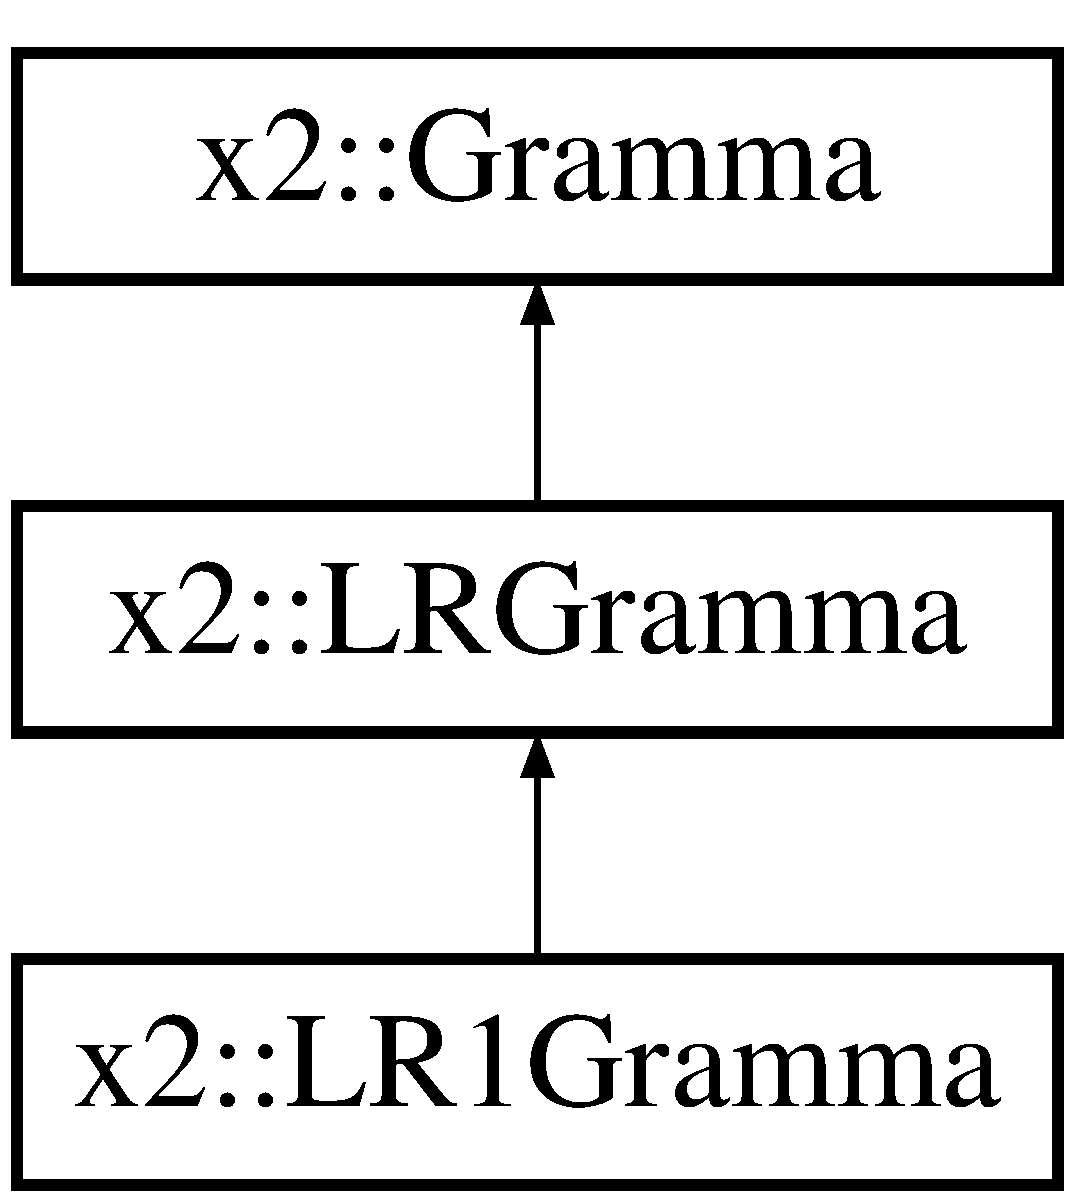
\includegraphics[height=3.000000cm]{classx2_1_1_gramma}
\end{center}
\end{figure}
\subsection*{Public Types}
\begin{DoxyCompactItemize}
\item 
\mbox{\Hypertarget{classx2_1_1_gramma_aa8b50e42698370df0a3dbe44e8c6f182}\label{classx2_1_1_gramma_aa8b50e42698370df0a3dbe44e8c6f182}} 
typedef \hyperlink{classx2_1_1_gramma}{Gramma} {\bfseries This}
\item 
\mbox{\Hypertarget{classx2_1_1_gramma_abbd7903e9220c50d0fc76a327b57fb1c}\label{classx2_1_1_gramma_abbd7903e9220c50d0fc76a327b57fb1c}} 
typedef std\+::map$<$ int, std\+::vector$<$ \hyperlink{classx2_1_1_gramma_sentence}{Gramma\+Sentence} $>$ $>$ {\bfseries Productions\+Type}
\item 
\mbox{\Hypertarget{classx2_1_1_gramma_a49dba600dd70cf11797ec8b887712cfd}\label{classx2_1_1_gramma_a49dba600dd70cf11797ec8b887712cfd}} 
typedef std\+::map$<$ int, std\+::set$<$ int $>$ $>$ {\bfseries Sets\+Type}
\item 
\mbox{\Hypertarget{classx2_1_1_gramma_aff012603885ff5f5618774fc210fb3d1}\label{classx2_1_1_gramma_aff012603885ff5f5618774fc210fb3d1}} 
typedef std\+::vector$<$ int $>$\+::size\+\_\+type {\bfseries size\+\_\+type}
\item 
\mbox{\Hypertarget{classx2_1_1_gramma_a03901eb5b196689b901fbf23e5bb9f0e}\label{classx2_1_1_gramma_a03901eb5b196689b901fbf23e5bb9f0e}} 
typedef std\+::map$<$ std\+::pair$<$ int, int $>$, std\+::set$<$ std\+::tuple$<$ int, int, int $>$ $>$ $>$ \hyperlink{classx2_1_1_gramma_a03901eb5b196689b901fbf23e5bb9f0e}{L\+R\+Corrupt\+Table\+Type}
\begin{DoxyCompactList}\small\item\em 带有冲突类型的\+L\+R分析表  请注意,L\+R分析表对于所有的\+L\+R文法都是通用的. tuple$<$int,int,int$>$ $<$i,j, action$>$ \end{DoxyCompactList}\item 
\mbox{\Hypertarget{classx2_1_1_gramma_a33681053b045219ea58cc68c3faa4975}\label{classx2_1_1_gramma_a33681053b045219ea58cc68c3faa4975}} 
typedef std\+::map$<$ std\+::pair$<$ int, int $>$, std\+::tuple$<$ int, int, int $>$ $>$ \hyperlink{classx2_1_1_gramma_a33681053b045219ea58cc68c3faa4975}{L\+R\+Analyze\+Table\+Type}
\begin{DoxyCompactList}\small\item\em 不带冲突的\+L\+R分析表,也称为标准的分析表 \end{DoxyCompactList}\end{DoxyCompactItemize}
\subsection*{Public Member Functions}
\begin{DoxyCompactItemize}
\item 
\mbox{\Hypertarget{classx2_1_1_gramma_aaa8482a5cebd401c1d194bf9eae74622}\label{classx2_1_1_gramma_aaa8482a5cebd401c1d194bf9eae74622}} 
{\bfseries Gramma} (const \hyperlink{classx2_1_1_gramma_symbols}{Gramma\+Symbols} \&gsyms)
\item 
\mbox{\Hypertarget{classx2_1_1_gramma_a83a39b4b3d064dd01117cab3a3ff1292}\label{classx2_1_1_gramma_a83a39b4b3d064dd01117cab3a3ff1292}} 
{\bfseries Gramma} (\hyperlink{classx2_1_1_gramma_symbols}{Gramma\+Symbols} \&\&gsyms)
\item 
\mbox{\Hypertarget{classx2_1_1_gramma_af6646cc2b56c3757361c4353bbb5d4d7}\label{classx2_1_1_gramma_af6646cc2b56c3757361c4353bbb5d4d7}} 
{\bfseries Gramma} (const std\+::initializer\+\_\+list$<$ std\+::pair$<$ int, std\+::string $>$ $>$ \&list)
\item 
\mbox{\Hypertarget{classx2_1_1_gramma_ad808555763361340d4d5ac83b21cae59}\label{classx2_1_1_gramma_ad808555763361340d4d5ac83b21cae59}} 
{\bfseries Gramma} (const std\+::string \&file)
\item 
\mbox{\Hypertarget{classx2_1_1_gramma_abc2824d9f948e57df12e62668872953b}\label{classx2_1_1_gramma_abc2824d9f948e57df12e62668872953b}} 
{\bfseries Gramma} (std\+::istream \&in)
\item 
\mbox{\Hypertarget{classx2_1_1_gramma_a4951974a0021d5ba56b32d75d8de4e53}\label{classx2_1_1_gramma_a4951974a0021d5ba56b32d75d8de4e53}} 
{\bfseries Gramma} (const std\+::initializer\+\_\+list$<$ std\+::pair$<$ int, std\+::string $>$ $>$ \&list, const std\+::initializer\+\_\+list$<$ std\+::pair$<$ int, \hyperlink{classx2_1_1_gramma_sentence}{Gramma\+Sentence} $>$ $>$ \&prodlist)
\item 
\mbox{\Hypertarget{classx2_1_1_gramma_aeab98669a1cc0e99274334dea8148f2a}\label{classx2_1_1_gramma_aeab98669a1cc0e99274334dea8148f2a}} 
{\bfseries Gramma} (const std\+::initializer\+\_\+list$<$ std\+::pair$<$ std\+::string, std\+::initializer\+\_\+list$<$ std\+::string $>$$>$$>$ \&prodlist)
\item 
\mbox{\Hypertarget{classx2_1_1_gramma_abd5c0c3cb506b2261e9c5af2d243f27b}\label{classx2_1_1_gramma_abd5c0c3cb506b2261e9c5af2d243f27b}} 
{\bfseries Gramma} (const std\+::vector$<$ std\+::pair$<$ std\+::string, std\+::vector$<$ std\+::string $>$$>$$>$ \&prodlist)
\item 
\mbox{\Hypertarget{classx2_1_1_gramma_af5e2d1e16f16be36dab8d5caed577bb3}\label{classx2_1_1_gramma_af5e2d1e16f16be36dab8d5caed577bb3}} 
{\bfseries Gramma} (std\+::initializer\+\_\+list$<$ std\+::string $>$ list)
\item 
\mbox{\Hypertarget{classx2_1_1_gramma_a32aff8f7801e9247ad2b9e54343c06aa}\label{classx2_1_1_gramma_a32aff8f7801e9247ad2b9e54343c06aa}} 
{\bfseries Gramma} (const std\+::vector$<$ std\+::string $>$ \&list)
\item 
\mbox{\Hypertarget{classx2_1_1_gramma_ae2f19aee6d2718fafb04cad678519e4a}\label{classx2_1_1_gramma_ae2f19aee6d2718fafb04cad678519e4a}} 
void {\bfseries add\+Production} (int i, const \hyperlink{classx2_1_1_gramma_sentence}{Gramma\+Sentence} \&gs)
\item 
\mbox{\Hypertarget{classx2_1_1_gramma_ace0d616133f9cd0b8ed81d7e98963f34}\label{classx2_1_1_gramma_ace0d616133f9cd0b8ed81d7e98963f34}} 
void {\bfseries add\+Production} (int i, \hyperlink{classx2_1_1_gramma_sentence}{Gramma\+Sentence} \&\&gs)
\item 
void \hyperlink{classx2_1_1_gramma_aaf4cbec7886ba7eaf878ca75a517e4e0}{add\+Production} (const std\+::string \&head, const std\+::vector$<$ std\+::string $>$ \&gs)
\item 
void \hyperlink{classx2_1_1_gramma_a86ff823a6b5aefacbc9a024414c078d8}{add\+Production} (const std\+::string \&head, const std\+::initializer\+\_\+list$<$ std\+::string $>$ \&gs)
\item 
\mbox{\Hypertarget{classx2_1_1_gramma_ab1701d83a618434e4025b42d59c3ed05}\label{classx2_1_1_gramma_ab1701d83a618434e4025b42d59c3ed05}} 
void {\bfseries add\+Production} (const std\+::string \&all)
\item 
\mbox{\Hypertarget{classx2_1_1_gramma_a10072e9945425e348fe164ae11dbd48e}\label{classx2_1_1_gramma_a10072e9945425e348fe164ae11dbd48e}} 
bool {\bfseries can\+Symbol\+Empty} (int i)
\item 
\mbox{\Hypertarget{classx2_1_1_gramma_a3ba8caf8e40ce5ce3e02fadd7fed0309}\label{classx2_1_1_gramma_a3ba8caf8e40ce5ce3e02fadd7fed0309}} 
bool {\bfseries can\+Sentence\+Empty} (const \hyperlink{classx2_1_1_gramma_sentence}{Gramma\+Sentence} \&s)
\item 
\mbox{\Hypertarget{classx2_1_1_gramma_ade7340fc0ee5e8514314465d5cae3348}\label{classx2_1_1_gramma_ade7340fc0ee5e8514314465d5cae3348}} 
bool {\bfseries can\+Sentence\+Empty} (const \hyperlink{classx2_1_1_gramma_sentence}{Gramma\+Sentence} \&s, int end)
\item 
\mbox{\Hypertarget{classx2_1_1_gramma_a11f1d43bcba6ed42c3bc6771745eb9c5}\label{classx2_1_1_gramma_a11f1d43bcba6ed42c3bc6771745eb9c5}} 
bool {\bfseries can\+Sentence\+Empty} (const \hyperlink{classx2_1_1_gramma_sentence}{Gramma\+Sentence} \&s, int start, int end)
\item 
\mbox{\Hypertarget{classx2_1_1_gramma_ae3eaf6c1a28873ca324ec3cc33f3e47c}\label{classx2_1_1_gramma_ae3eaf6c1a28873ca324ec3cc33f3e47c}} 
A\+S\+\_\+\+M\+A\+C\+RO const std\+::vector$<$ \hyperlink{classx2_1_1_gramma_sentence}{Gramma\+Sentence} $>$ \& {\bfseries get\+Right\+Sentences} (int i) const
\item 
\mbox{\Hypertarget{classx2_1_1_gramma_a1d34706fe75ade7df4e0e45800d9a652}\label{classx2_1_1_gramma_a1d34706fe75ade7df4e0e45800d9a652}} 
A\+S\+\_\+\+M\+A\+C\+RO std\+::vector$<$ \hyperlink{classx2_1_1_gramma_sentence}{Gramma\+Sentence} $>$ \& {\bfseries get\+Right\+Sentences} (int i)
\item 
void \hyperlink{classx2_1_1_gramma_aa5e24a49dbf499af546703b594ef4a51}{replace\+First\+Production} (int i, const int j)
\item 
\mbox{\Hypertarget{classx2_1_1_gramma_a621ddb8f04f2c00e747940bde3bbf6e6}\label{classx2_1_1_gramma_a621ddb8f04f2c00e747940bde3bbf6e6}} 
void {\bfseries reduce\+Left\+Recursive} ()
\item 
\mbox{\Hypertarget{classx2_1_1_gramma_ab87bf7edf41374f02def88a3ebcb4407}\label{classx2_1_1_gramma_ab87bf7edf41374f02def88a3ebcb4407}} 
void {\bfseries eliminate\+Self\+Deduction} (int i)
\item 
\mbox{\Hypertarget{classx2_1_1_gramma_a1a94a73d06f42e99630d434f79593bdc}\label{classx2_1_1_gramma_a1a94a73d06f42e99630d434f79593bdc}} 
A\+S\+\_\+\+M\+A\+C\+RO void {\bfseries eliminate\+Self\+Deduction} ()
\item 
\mbox{\Hypertarget{classx2_1_1_gramma_a5fb5250196eadcb35ab2f3c33ffaee4a}\label{classx2_1_1_gramma_a5fb5250196eadcb35ab2f3c33ffaee4a}} 
void {\bfseries eliminate\+Duplication} (int i)
\item 
\mbox{\Hypertarget{classx2_1_1_gramma_ac9f8249e01fe17a2b2fd6cc1e4e7155a}\label{classx2_1_1_gramma_ac9f8249e01fe17a2b2fd6cc1e4e7155a}} 
A\+S\+\_\+\+M\+A\+C\+RO void {\bfseries eliminate\+Duplication} ()
\item 
void \hyperlink{classx2_1_1_gramma_abc0b45a3d37e2955bc89d74bb5234697}{reduce\+Direct\+Left\+Recursive} (int i)
\item 
\mbox{\Hypertarget{classx2_1_1_gramma_ab0c313d702258f7d93aad0faf2095eb0}\label{classx2_1_1_gramma_ab0c313d702258f7d93aad0faf2095eb0}} 
A\+S\+\_\+\+M\+A\+C\+RO void {\bfseries reduce\+Direct\+Left\+Recursive} ()
\item 
\mbox{\Hypertarget{classx2_1_1_gramma_a0f5c977a9bcb4b8547fb41e2085b8c70}\label{classx2_1_1_gramma_a0f5c977a9bcb4b8547fb41e2085b8c70}} 
A\+S\+\_\+\+M\+A\+C\+RO void {\bfseries reduce\+Left\+Factor} ()
\item 
\mbox{\Hypertarget{classx2_1_1_gramma_a326ea520b5348ec08e6e6f496220a080}\label{classx2_1_1_gramma_a326ea520b5348ec08e6e6f496220a080}} 
A\+S\+\_\+\+M\+A\+C\+RO void {\bfseries reduce\+Left\+Factor} (int i)
\item 
int \hyperlink{classx2_1_1_gramma_a883d11029de8fb73053b478870b78c89}{reduce} (std\+::vector$<$ \hyperlink{classx2_1_1_gramma_sentence}{Gramma\+Sentence} $>$ \&data, const std\+::string \&varname, int start, int end, std\+::vector$<$ int $>$ \&subset)
\item 
\mbox{\Hypertarget{classx2_1_1_gramma_a242995260a76097e8a342b362106dff4}\label{classx2_1_1_gramma_a242995260a76097e8a342b362106dff4}} 
void {\bfseries reduce\+Left\+Factor} (std\+::vector$<$ \hyperlink{classx2_1_1_gramma_sentence}{Gramma\+Sentence} $>$ \&data, const std\+::string \&varname, int i)
\item 
std\+::vector$<$ int $>$ \hyperlink{classx2_1_1_gramma_a17a55403158293775921697a94a7f2c1}{get\+Productions\+Head} () const
\item 
void \hyperlink{classx2_1_1_gramma_a15e7c86a1dae673945a108f1bf2fb80c}{reduce\+Left\+Factor} (int i, int j)
\item 
\mbox{\Hypertarget{classx2_1_1_gramma_abc71debab97cec29b1a417c6801ca73a}\label{classx2_1_1_gramma_abc71debab97cec29b1a417c6801ca73a}} 
Sets\+Type {\bfseries calc\+First} ()
\item 
\mbox{\Hypertarget{classx2_1_1_gramma_a4f587bc53e41f69627c7b30454813a20}\label{classx2_1_1_gramma_a4f587bc53e41f69627c7b30454813a20}} 
std\+::set$<$ int $>$ {\bfseries calc\+First} (const \hyperlink{classx2_1_1_gramma_sentence}{Gramma\+Sentence} \&gs, int start, int end, const Sets\+Type \&firstset)
\item 
\mbox{\Hypertarget{classx2_1_1_gramma_a7936a7fb2f169fb995c55f0b114098a3}\label{classx2_1_1_gramma_a7936a7fb2f169fb995c55f0b114098a3}} 
Sets\+Type {\bfseries calc\+Follow} (const Sets\+Type \&firstset, int start\+Sym, int end\+Sym)
\item 
\mbox{\Hypertarget{classx2_1_1_gramma_aa3a32e4425700a215bf112ccb8a2cf6b}\label{classx2_1_1_gramma_aa3a32e4425700a215bf112ccb8a2cf6b}} 
\hyperlink{classx2_1_1_gramma}{Gramma} {\bfseries duplicate} ()
\item 
\mbox{\Hypertarget{classx2_1_1_gramma_a48f86b362ff1dc0d66b950032ff8de8a}\label{classx2_1_1_gramma_a48f86b362ff1dc0d66b950032ff8de8a}} 
\hyperlink{classx2_1_1_gramma}{Gramma} {\bfseries duplicate\+Share\+Symbols} ()
\item 
\mbox{\Hypertarget{classx2_1_1_gramma_aaf454e5652ec9d278950d0db09506798}\label{classx2_1_1_gramma_aaf454e5652ec9d278950d0db09506798}} 
A\+S\+\_\+\+M\+A\+C\+RO std\+::string {\bfseries to\+String} () const
\item 
\mbox{\Hypertarget{classx2_1_1_gramma_aabbb04e38d5027b21ae2ab03bfbfaa17}\label{classx2_1_1_gramma_aabbb04e38d5027b21ae2ab03bfbfaa17}} 
A\+S\+\_\+\+M\+A\+C\+RO std\+::string {\bfseries to\+String} (int i) const
\item 
\mbox{\Hypertarget{classx2_1_1_gramma_a8f79c3c8284ad9a7b2a080e0cc327137}\label{classx2_1_1_gramma_a8f79c3c8284ad9a7b2a080e0cc327137}} 
A\+S\+\_\+\+M\+A\+C\+RO std\+::string {\bfseries to\+String} (const \hyperlink{classx2_1_1_gramma_sentence}{Gramma\+Sentence} \&gs) const
\item 
\mbox{\Hypertarget{classx2_1_1_gramma_a6853c16fd634bad1051ab8f8d212f3b8}\label{classx2_1_1_gramma_a6853c16fd634bad1051ab8f8d212f3b8}} 
A\+S\+\_\+\+M\+A\+C\+RO std\+::string {\bfseries to\+String} (int i, const std\+::vector$<$ \hyperlink{classx2_1_1_gramma_sentence}{Gramma\+Sentence} $>$ \&gss) const
\item 
\mbox{\Hypertarget{classx2_1_1_gramma_a0027de55c6f5cba74472f907aee33c61}\label{classx2_1_1_gramma_a0027de55c6f5cba74472f907aee33c61}} 
A\+S\+\_\+\+M\+A\+C\+RO std\+::string {\bfseries to\+String} (int i, int j) const
\item 
std\+::string \hyperlink{classx2_1_1_gramma_a04fc8a9d7e0dcc709706ac9bc117fb35}{to\+String} (const Sets\+Type \&set) const
\item 
\mbox{\Hypertarget{classx2_1_1_gramma_ab88c409d2f637b743e224d5bf12bdc2c}\label{classx2_1_1_gramma_ab88c409d2f637b743e224d5bf12bdc2c}} 
std\+::string {\bfseries to\+String} (const std\+::set$<$ int $>$ \&set) const
\item 
\mbox{\Hypertarget{classx2_1_1_gramma_a52c38fc9e80328e3779f41df5717e33e}\label{classx2_1_1_gramma_a52c38fc9e80328e3779f41df5717e33e}} 
A\+S\+\_\+\+M\+A\+C\+RO const \hyperlink{classx2_1_1_gramma_symbols}{Gramma\+Symbols} \& {\bfseries get\+Gramma\+Symbols} ()
\end{DoxyCompactItemize}
\subsection*{Static Public Member Functions}
\begin{DoxyCompactItemize}
\item 
\mbox{\Hypertarget{classx2_1_1_gramma_a803bd74e9d0c3d7199bc03439b1df537}\label{classx2_1_1_gramma_a803bd74e9d0c3d7199bc03439b1df537}} 
static \hyperlink{classx2_1_1_gramma_a33681053b045219ea58cc68c3faa4975}{L\+R\+Analyze\+Table\+Type} \hyperlink{classx2_1_1_gramma_a803bd74e9d0c3d7199bc03439b1df537}{convert\+Corrupt\+To\+Standard\+Simply} (const \hyperlink{classx2_1_1_gramma_a03901eb5b196689b901fbf23e5bb9f0e}{L\+R\+Corrupt\+Table\+Type} \&table)
\begin{DoxyCompactList}\small\item\em 提供一个最简单的将冲突的分析表转换成标准分析表的方法:仅仅保留第一项 \end{DoxyCompactList}\end{DoxyCompactItemize}
\subsection*{Public Attributes}
\begin{DoxyCompactItemize}
\item 
\mbox{\Hypertarget{classx2_1_1_gramma_af1a00aadbdd36bb81faf35c739eca913}\label{classx2_1_1_gramma_af1a00aadbdd36bb81faf35c739eca913}} 
\hyperlink{classx2_1_1_gramma_symbols}{Gramma\+Symbols} {\bfseries gsyms}
\end{DoxyCompactItemize}
\subsection*{Protected Attributes}
\begin{DoxyCompactItemize}
\item 
\mbox{\Hypertarget{classx2_1_1_gramma_a0b545b47424e8e783b21e84ac746eb05}\label{classx2_1_1_gramma_a0b545b47424e8e783b21e84ac746eb05}} 
Productions\+Type {\bfseries prods}
\end{DoxyCompactItemize}


\subsection{Detailed Description}
LL Utilities are automatically loadeed Gramma状态约定: 如果syms中存在一个非终结符号,则prods必然包含至少一个产生式(统一性) prods中的所有产生式,左部只能来自syms表的非终结符,右部只能是syms符号的一个组合

First集中只能含有空符号或者终结符

我的优化的原意是消除冗余,但是现在看来没有那个必要了

some conditions\+: S -\/$>$ S 毫无意义, 会在消除直接左递归的过程中消除掉,但是这属于循环推导,可能会引起消除间接左递归的失败 

\subsection{Member Function Documentation}
\mbox{\Hypertarget{classx2_1_1_gramma_aaf4cbec7886ba7eaf878ca75a517e4e0}\label{classx2_1_1_gramma_aaf4cbec7886ba7eaf878ca75a517e4e0}} 
\index{x2\+::\+Gramma@{x2\+::\+Gramma}!add\+Production@{add\+Production}}
\index{add\+Production@{add\+Production}!x2\+::\+Gramma@{x2\+::\+Gramma}}
\subsubsection{\texorpdfstring{add\+Production()}{addProduction()}\hspace{0.1cm}{\footnotesize\ttfamily [1/2]}}
{\footnotesize\ttfamily void x2\+::\+Gramma\+::add\+Production (\begin{DoxyParamCaption}\item[{const std\+::string \&}]{head,  }\item[{const std\+::vector$<$ std\+::string $>$ \&}]{gs }\end{DoxyParamCaption})\hspace{0.3cm}{\ttfamily [inline]}}

added 2017-\/04-\/21 21\+:49\+:40 \mbox{\Hypertarget{classx2_1_1_gramma_a86ff823a6b5aefacbc9a024414c078d8}\label{classx2_1_1_gramma_a86ff823a6b5aefacbc9a024414c078d8}} 
\index{x2\+::\+Gramma@{x2\+::\+Gramma}!add\+Production@{add\+Production}}
\index{add\+Production@{add\+Production}!x2\+::\+Gramma@{x2\+::\+Gramma}}
\subsubsection{\texorpdfstring{add\+Production()}{addProduction()}\hspace{0.1cm}{\footnotesize\ttfamily [2/2]}}
{\footnotesize\ttfamily void x2\+::\+Gramma\+::add\+Production (\begin{DoxyParamCaption}\item[{const std\+::string \&}]{head,  }\item[{const std\+::initializer\+\_\+list$<$ std\+::string $>$ \&}]{gs }\end{DoxyParamCaption})\hspace{0.3cm}{\ttfamily [inline]}}

added 2017-\/04-\/21 21\+:49\+:47 \mbox{\Hypertarget{classx2_1_1_gramma_a17a55403158293775921697a94a7f2c1}\label{classx2_1_1_gramma_a17a55403158293775921697a94a7f2c1}} 
\index{x2\+::\+Gramma@{x2\+::\+Gramma}!get\+Productions\+Head@{get\+Productions\+Head}}
\index{get\+Productions\+Head@{get\+Productions\+Head}!x2\+::\+Gramma@{x2\+::\+Gramma}}
\subsubsection{\texorpdfstring{get\+Productions\+Head()}{getProductionsHead()}}
{\footnotesize\ttfamily std\+::vector$<$ int $>$ x2\+::\+Gramma\+::get\+Productions\+Head (\begin{DoxyParamCaption}{ }\end{DoxyParamCaption}) const}

获得当前的产生式的所有键,以避免发生prods修改时,迭代器失效 \mbox{\Hypertarget{classx2_1_1_gramma_a883d11029de8fb73053b478870b78c89}\label{classx2_1_1_gramma_a883d11029de8fb73053b478870b78c89}} 
\index{x2\+::\+Gramma@{x2\+::\+Gramma}!reduce@{reduce}}
\index{reduce@{reduce}!x2\+::\+Gramma@{x2\+::\+Gramma}}
\subsubsection{\texorpdfstring{reduce()}{reduce()}}
{\footnotesize\ttfamily int x2\+::\+Gramma\+::reduce (\begin{DoxyParamCaption}\item[{std\+::vector$<$ \hyperlink{classx2_1_1_gramma_sentence}{Gramma\+Sentence} $>$ \&}]{data,  }\item[{const std\+::string \&}]{varname,  }\item[{int}]{start,  }\item[{int}]{end,  }\item[{std\+::vector$<$ int $>$ \&}]{subset }\end{DoxyParamCaption})}

start from start, end at end,not including end \mbox{\Hypertarget{classx2_1_1_gramma_abc0b45a3d37e2955bc89d74bb5234697}\label{classx2_1_1_gramma_abc0b45a3d37e2955bc89d74bb5234697}} 
\index{x2\+::\+Gramma@{x2\+::\+Gramma}!reduce\+Direct\+Left\+Recursive@{reduce\+Direct\+Left\+Recursive}}
\index{reduce\+Direct\+Left\+Recursive@{reduce\+Direct\+Left\+Recursive}!x2\+::\+Gramma@{x2\+::\+Gramma}}
\subsubsection{\texorpdfstring{reduce\+Direct\+Left\+Recursive()}{reduceDirectLeftRecursive()}}
{\footnotesize\ttfamily void x2\+::\+Gramma\+::reduce\+Direct\+Left\+Recursive (\begin{DoxyParamCaption}\item[{int}]{i }\end{DoxyParamCaption})}

将i归为两类:以s开头和不以s开头 \mbox{\Hypertarget{classx2_1_1_gramma_a15e7c86a1dae673945a108f1bf2fb80c}\label{classx2_1_1_gramma_a15e7c86a1dae673945a108f1bf2fb80c}} 
\index{x2\+::\+Gramma@{x2\+::\+Gramma}!reduce\+Left\+Factor@{reduce\+Left\+Factor}}
\index{reduce\+Left\+Factor@{reduce\+Left\+Factor}!x2\+::\+Gramma@{x2\+::\+Gramma}}
\subsubsection{\texorpdfstring{reduce\+Left\+Factor()}{reduceLeftFactor()}}
{\footnotesize\ttfamily void x2\+::\+Gramma\+::reduce\+Left\+Factor (\begin{DoxyParamCaption}\item[{int}]{i,  }\item[{int}]{j }\end{DoxyParamCaption})}

消除 i中所有以j开头的左因子 查找以最长公共前缀,将前缀后面的串替换成一个新的语法变量,然后删除重复的串

引入的语法变量名称为原变量加上\textquotesingle{} \mbox{\Hypertarget{classx2_1_1_gramma_aa5e24a49dbf499af546703b594ef4a51}\label{classx2_1_1_gramma_aa5e24a49dbf499af546703b594ef4a51}} 
\index{x2\+::\+Gramma@{x2\+::\+Gramma}!replace\+First\+Production@{replace\+First\+Production}}
\index{replace\+First\+Production@{replace\+First\+Production}!x2\+::\+Gramma@{x2\+::\+Gramma}}
\subsubsection{\texorpdfstring{replace\+First\+Production()}{replaceFirstProduction()}}
{\footnotesize\ttfamily void x2\+::\+Gramma\+::replace\+First\+Production (\begin{DoxyParamCaption}\item[{int}]{i,  }\item[{const int}]{j }\end{DoxyParamCaption})}

对 i -\/$>$ j ..进行替换 \mbox{\Hypertarget{classx2_1_1_gramma_a04fc8a9d7e0dcc709706ac9bc117fb35}\label{classx2_1_1_gramma_a04fc8a9d7e0dcc709706ac9bc117fb35}} 
\index{x2\+::\+Gramma@{x2\+::\+Gramma}!to\+String@{to\+String}}
\index{to\+String@{to\+String}!x2\+::\+Gramma@{x2\+::\+Gramma}}
\subsubsection{\texorpdfstring{to\+String()}{toString()}}
{\footnotesize\ttfamily std\+::string x2\+::\+Gramma\+::to\+String (\begin{DoxyParamCaption}\item[{const Sets\+Type \&}]{set }\end{DoxyParamCaption}) const}

for F\+O\+L\+L\+OW \& F\+I\+R\+ST 

The documentation for this class was generated from the following files\+:\begin{DoxyCompactItemize}
\item 
D\+:/\+Pool/eclipse-\/workspace/compiler-\/debug/include/Gramma\+Utils.\+h\item 
D\+:/\+Pool/eclipse-\/workspace/compiler-\/debug/src/Gramma\+Utils.\+cpp\end{DoxyCompactItemize}

\hypertarget{classx2_1_1_gramma_sentence}{}\section{x2\+:\+:Gramma\+Sentence Class Reference}
\label{classx2_1_1_gramma_sentence}\index{x2\+::\+Gramma\+Sentence@{x2\+::\+Gramma\+Sentence}}


{\ttfamily \#include $<$Gramma\+Utils.\+h$>$}

\subsection*{Public Types}
\begin{DoxyCompactItemize}
\item 
\mbox{\Hypertarget{classx2_1_1_gramma_sentence_a2ac136621c50e96f7d126eec257ebddd}\label{classx2_1_1_gramma_sentence_a2ac136621c50e96f7d126eec257ebddd}} 
typedef std\+::vector$<$ int $>$ {\bfseries Syms\+List\+Type}
\item 
\mbox{\Hypertarget{classx2_1_1_gramma_sentence_abece966f6435f072c4535f81b8f58115}\label{classx2_1_1_gramma_sentence_abece966f6435f072c4535f81b8f58115}} 
typedef Syms\+List\+Type\+::size\+\_\+type {\bfseries size\+\_\+type}
\end{DoxyCompactItemize}
\subsection*{Public Member Functions}
\begin{DoxyCompactItemize}
\item 
\mbox{\Hypertarget{classx2_1_1_gramma_sentence_aebcf626920630103d5f5a48a00eb57a4}\label{classx2_1_1_gramma_sentence_aebcf626920630103d5f5a48a00eb57a4}} 
{\bfseries Gramma\+Sentence} (\hyperlink{classx2_1_1_gramma_sentence}{Gramma\+Sentence} \&\&gs)=default
\item 
\mbox{\Hypertarget{classx2_1_1_gramma_sentence_a90e50f2cf45081bc11d5ff18ab7913b8}\label{classx2_1_1_gramma_sentence_a90e50f2cf45081bc11d5ff18ab7913b8}} 
{\bfseries Gramma\+Sentence} (const \hyperlink{classx2_1_1_gramma_sentence}{Gramma\+Sentence} \&gs)=default
\item 
\mbox{\Hypertarget{classx2_1_1_gramma_sentence_aff4e3d88d7166fc7a3748df2b66109c2}\label{classx2_1_1_gramma_sentence_aff4e3d88d7166fc7a3748df2b66109c2}} 
{\bfseries Gramma\+Sentence} (const Syms\+List\+Type \&slist)
\item 
\mbox{\Hypertarget{classx2_1_1_gramma_sentence_aa407f65f300d881bc9225d12488325ea}\label{classx2_1_1_gramma_sentence_aa407f65f300d881bc9225d12488325ea}} 
{\bfseries Gramma\+Sentence} (Syms\+List\+Type \&\&slist)
\item 
\mbox{\Hypertarget{classx2_1_1_gramma_sentence_a1f857ae143012e35a8021714c9236ead}\label{classx2_1_1_gramma_sentence_a1f857ae143012e35a8021714c9236ead}} 
{\bfseries Gramma\+Sentence} (std\+::initializer\+\_\+list$<$ int $>$ \&\&list)
\item 
\mbox{\Hypertarget{classx2_1_1_gramma_sentence_acce42463db9a6c6d78454f49c579ac11}\label{classx2_1_1_gramma_sentence_acce42463db9a6c6d78454f49c579ac11}} 
{\bfseries Gramma\+Sentence} (const std\+::initializer\+\_\+list$<$ int $>$ \&list)
\item 
\mbox{\Hypertarget{classx2_1_1_gramma_sentence_ac71133dec3e7bb06253e32982e7add31}\label{classx2_1_1_gramma_sentence_ac71133dec3e7bb06253e32982e7add31}} 
\hyperlink{classx2_1_1_gramma_sentence}{Gramma\+Sentence} \& {\bfseries operator=} (const \hyperlink{classx2_1_1_gramma_sentence}{Gramma\+Sentence} \&gs)
\item 
\mbox{\Hypertarget{classx2_1_1_gramma_sentence_a695af7767ca769144cbaafc7714d7976}\label{classx2_1_1_gramma_sentence_a695af7767ca769144cbaafc7714d7976}} 
void {\bfseries replace\+First} (const \hyperlink{classx2_1_1_gramma_sentence}{Gramma\+Sentence} \&gs, int empty)
\item 
\mbox{\Hypertarget{classx2_1_1_gramma_sentence_aaa3adf3d7d6642e08adb7c619d1a3c1f}\label{classx2_1_1_gramma_sentence_aaa3adf3d7d6642e08adb7c619d1a3c1f}} 
std\+::vector$<$ \hyperlink{classx2_1_1_gramma_sentence}{Gramma\+Sentence} $>$ {\bfseries replace\+First} (const std\+::vector$<$ \hyperlink{classx2_1_1_gramma_sentence}{Gramma\+Sentence} $>$ \&vgs, int empty)
\item 
\mbox{\Hypertarget{classx2_1_1_gramma_sentence_ae9c2408b6a175986d70914139ba08ab4}\label{classx2_1_1_gramma_sentence_ae9c2408b6a175986d70914139ba08ab4}} 
\hyperlink{classx2_1_1_gramma_sentence}{Gramma\+Sentence} {\bfseries duplicate} () const
\item 
\mbox{\Hypertarget{classx2_1_1_gramma_sentence_a4312f5a83549fd228e1b119b0969a142}\label{classx2_1_1_gramma_sentence_a4312f5a83549fd228e1b119b0969a142}} 
A\+S\+\_\+\+M\+A\+C\+RO int {\bfseries get\+First\+Symbol} () const
\item 
\mbox{\Hypertarget{classx2_1_1_gramma_sentence_abe7ce37e3ae87d5b593b3521eccabe5a}\label{classx2_1_1_gramma_sentence_abe7ce37e3ae87d5b593b3521eccabe5a}} 
A\+S\+\_\+\+M\+A\+C\+RO bool {\bfseries starts\+With} (int i) const
\item 
\mbox{\Hypertarget{classx2_1_1_gramma_sentence_a07e2e2a7bf13008a55c9a71f1e3ccbb9}\label{classx2_1_1_gramma_sentence_a07e2e2a7bf13008a55c9a71f1e3ccbb9}} 
A\+S\+\_\+\+M\+A\+C\+RO size\+\_\+type {\bfseries get\+Length} () const
\item 
\mbox{\Hypertarget{classx2_1_1_gramma_sentence_a3e6c91515206b17988bd9dab613976b2}\label{classx2_1_1_gramma_sentence_a3e6c91515206b17988bd9dab613976b2}} 
void {\bfseries push\+\_\+back} (int i)
\end{DoxyCompactItemize}
\subsection*{Public Attributes}
\begin{DoxyCompactItemize}
\item 
\mbox{\Hypertarget{classx2_1_1_gramma_sentence_a425eeca4d66cc4c28544b3b6f1027b06}\label{classx2_1_1_gramma_sentence_a425eeca4d66cc4c28544b3b6f1027b06}} 
Syms\+List\+Type {\bfseries syms}
\end{DoxyCompactItemize}


\subsection{Detailed Description}
Gramma\+Sentence约定: 如果\+Gramma\+Sentence为空产生式,则含有语法变量 S\+Y\+M\+\_\+\+E\+M\+P\+TY 长度至少为1 

The documentation for this class was generated from the following files\+:\begin{DoxyCompactItemize}
\item 
D\+:/\+Pool/eclipse-\/workspace/compiler-\/debug/include/Gramma\+Utils.\+h\item 
D\+:/\+Pool/eclipse-\/workspace/compiler-\/debug/src/Gramma\+Utils.\+cpp\end{DoxyCompactItemize}

\hypertarget{classx2_1_1_gramma_symbols}{}\section{x2\+:\+:Gramma\+Symbols Class Reference}
\label{classx2_1_1_gramma_symbols}\index{x2\+::\+Gramma\+Symbols@{x2\+::\+Gramma\+Symbols}}


{\ttfamily \#include $<$Gramma\+Utils.\+h$>$}

\subsection*{Public Types}
\begin{DoxyCompactItemize}
\item 
\mbox{\Hypertarget{classx2_1_1_gramma_symbols_aa2d271a9d4d8adb95a97f45c743ad322}\label{classx2_1_1_gramma_symbols_aa2d271a9d4d8adb95a97f45c743ad322}} 
enum {\bfseries T\+Y\+P\+E\+\_\+\+D\+EF} \{ {\bfseries T\+Y\+P\+E\+\_\+\+T\+E\+RM}, 
{\bfseries T\+Y\+P\+E\+\_\+\+V\+AR}, 
{\bfseries T\+Y\+P\+E\+\_\+\+E\+M\+P\+TY}, 
{\bfseries T\+Y\+P\+E\+\_\+\+U\+N\+D\+E\+F\+I\+N\+ED}
 \}
\item 
\mbox{\Hypertarget{classx2_1_1_gramma_symbols_a88f776185c38f99d90dfe88faf406486}\label{classx2_1_1_gramma_symbols_a88f776185c38f99d90dfe88faf406486}} 
typedef std\+::map$<$ int, int $>$ {\bfseries Type\+Info}
\item 
\mbox{\Hypertarget{classx2_1_1_gramma_symbols_ac78d9a23d6a926093a2269d5f4fddc2c}\label{classx2_1_1_gramma_symbols_ac78d9a23d6a926093a2269d5f4fddc2c}} 
typedef std\+::map$<$ int, std\+::string $>$ {\bfseries Type\+String}
\item 
\mbox{\Hypertarget{classx2_1_1_gramma_symbols_a3e471289e4e8bdf147e0e12b0f283ce6}\label{classx2_1_1_gramma_symbols_a3e471289e4e8bdf147e0e12b0f283ce6}} 
typedef \hyperlink{classx2_1_1_gramma_symbols}{Gramma\+Symbols} {\bfseries This}
\end{DoxyCompactItemize}
\subsection*{Public Member Functions}
\begin{DoxyCompactItemize}
\item 
\mbox{\Hypertarget{classx2_1_1_gramma_symbols_a3c821b367628262c5c5f2a0dda4250b3}\label{classx2_1_1_gramma_symbols_a3c821b367628262c5c5f2a0dda4250b3}} 
{\bfseries Gramma\+Symbols} (const std\+::string \&empty\+String=E\+M\+P\+T\+Y\+\_\+\+S\+T\+R\+I\+NG)
\item 
\mbox{\Hypertarget{classx2_1_1_gramma_symbols_ac90febd608ebef059fa29ea52a588518}\label{classx2_1_1_gramma_symbols_ac90febd608ebef059fa29ea52a588518}} 
{\bfseries Gramma\+Symbols} (const \hyperlink{classx2_1_1_gramma_symbols}{Gramma\+Symbols} \&gsyms)=default
\item 
\mbox{\Hypertarget{classx2_1_1_gramma_symbols_a891a249c01275bc3e1a31540b8a2d3b0}\label{classx2_1_1_gramma_symbols_a891a249c01275bc3e1a31540b8a2d3b0}} 
{\bfseries Gramma\+Symbols} (\hyperlink{classx2_1_1_gramma_symbols}{Gramma\+Symbols} \&\&gsyms)
\item 
\mbox{\Hypertarget{classx2_1_1_gramma_symbols_ae672047f559d8551d520d88622da7f63}\label{classx2_1_1_gramma_symbols_ae672047f559d8551d520d88622da7f63}} 
{\bfseries Gramma\+Symbols} (const std\+::initializer\+\_\+list$<$ std\+::pair$<$ int, std\+::string $>$ $>$ \&list)
\item 
\mbox{\Hypertarget{classx2_1_1_gramma_symbols_ae71d1c101cc5ed0d981434c7060f5efd}\label{classx2_1_1_gramma_symbols_ae71d1c101cc5ed0d981434c7060f5efd}} 
\hyperlink{classx2_1_1_gramma_symbols}{Gramma\+Symbols} \& {\bfseries operator=} (const \hyperlink{classx2_1_1_gramma_symbols}{Gramma\+Symbols} \&gs)
\item 
\mbox{\Hypertarget{classx2_1_1_gramma_symbols_af7bae01689e15f9aa7ff509f2a736999}\label{classx2_1_1_gramma_symbols_af7bae01689e15f9aa7ff509f2a736999}} 
\hyperlink{classx2_1_1_gramma_symbols}{Gramma\+Symbols} \& {\bfseries operator=} (\hyperlink{classx2_1_1_gramma_symbols}{Gramma\+Symbols} \&\&gs)
\item 
\mbox{\Hypertarget{classx2_1_1_gramma_symbols_a4ab0bdb81b834729a6487c421d33ef30}\label{classx2_1_1_gramma_symbols_a4ab0bdb81b834729a6487c421d33ef30}} 
A\+S\+\_\+\+M\+A\+C\+RO int {\bfseries get} (const std\+::string \&s) const
\item 
\mbox{\Hypertarget{classx2_1_1_gramma_symbols_a0d57500363cfa99756f71b04059fa806}\label{classx2_1_1_gramma_symbols_a0d57500363cfa99756f71b04059fa806}} 
A\+S\+\_\+\+M\+A\+C\+RO int {\bfseries get\+Add} (const std\+::string \&sym, const std\+::string \&type=\char`\"{}T\+E\+R\+M\+I\+N\+A\+T\+OR\char`\"{})
\item 
\mbox{\Hypertarget{classx2_1_1_gramma_symbols_aefe73ad5dbbda477272ccadfcc2ef84a}\label{classx2_1_1_gramma_symbols_aefe73ad5dbbda477272ccadfcc2ef84a}} 
A\+S\+\_\+\+M\+A\+C\+RO int {\bfseries get\+Add} (const std\+::string \&sym, int type)
\item 
int \hyperlink{classx2_1_1_gramma_symbols_ac7cb85affa4c6c9a6176ace01d6ed4b6}{add\+Replace} (const std\+::string \&sym, const std\+::string \&type=\char`\"{}T\+E\+R\+M\+I\+N\+A\+T\+OR\char`\"{})
\item 
\mbox{\Hypertarget{classx2_1_1_gramma_symbols_af183c98f51b9ea1982cf39314790e04f}\label{classx2_1_1_gramma_symbols_af183c98f51b9ea1982cf39314790e04f}} 
int {\bfseries add\+Replace} (const std\+::string \&sym, int type)
\item 
\mbox{\Hypertarget{classx2_1_1_gramma_symbols_ac6966547daf0c9009e27f5ceb1923c2c}\label{classx2_1_1_gramma_symbols_ac6966547daf0c9009e27f5ceb1923c2c}} 
A\+S\+\_\+\+M\+A\+C\+RO int {\bfseries get\+Empty} () const
\item 
\mbox{\Hypertarget{classx2_1_1_gramma_symbols_a23a09b16e7f63902ccd97cc94baabd97}\label{classx2_1_1_gramma_symbols_a23a09b16e7f63902ccd97cc94baabd97}} 
A\+S\+\_\+\+M\+A\+C\+RO bool {\bfseries is\+Symbol\+Empty} (const std\+::string \&sym) const
\item 
\mbox{\Hypertarget{classx2_1_1_gramma_symbols_a2c8b9e2d1df211b086e2fd678378165e}\label{classx2_1_1_gramma_symbols_a2c8b9e2d1df211b086e2fd678378165e}} 
A\+S\+\_\+\+M\+A\+C\+RO bool {\bfseries is\+Symbol\+Term} (const std\+::string \&sym) const
\item 
\mbox{\Hypertarget{classx2_1_1_gramma_symbols_a3e74a49ffb1765129d17863820ce743d}\label{classx2_1_1_gramma_symbols_a3e74a49ffb1765129d17863820ce743d}} 
A\+S\+\_\+\+M\+A\+C\+RO bool {\bfseries is\+Symbol\+Undefined} (const std\+::string \&sym) const
\item 
\mbox{\Hypertarget{classx2_1_1_gramma_symbols_a386ddcce4fecf5e158e6371e05c74bba}\label{classx2_1_1_gramma_symbols_a386ddcce4fecf5e158e6371e05c74bba}} 
A\+S\+\_\+\+M\+A\+C\+RO int {\bfseries get\+Symbol\+Type} (const std\+::string \&sym) const
\item 
\mbox{\Hypertarget{classx2_1_1_gramma_symbols_ae68863cdea90c8ae218fa65498a748d3}\label{classx2_1_1_gramma_symbols_ae68863cdea90c8ae218fa65498a748d3}} 
A\+S\+\_\+\+M\+A\+C\+RO int {\bfseries add\+Term} (const std\+::string \&s)
\item 
\mbox{\Hypertarget{classx2_1_1_gramma_symbols_a6ca7cacf622113005532d791c46116de}\label{classx2_1_1_gramma_symbols_a6ca7cacf622113005532d791c46116de}} 
A\+S\+\_\+\+M\+A\+C\+RO int {\bfseries add\+Var} (const std\+::string \&s)
\item 
\mbox{\Hypertarget{classx2_1_1_gramma_symbols_a21edf771f7aaec70f68986f9e3afa695}\label{classx2_1_1_gramma_symbols_a21edf771f7aaec70f68986f9e3afa695}} 
int {\bfseries add\+Empty} (const std\+::string \&s)
\item 
\mbox{\Hypertarget{classx2_1_1_gramma_symbols_ac6f411be6b4aacc787529f2dfda62206}\label{classx2_1_1_gramma_symbols_ac6f411be6b4aacc787529f2dfda62206}} 
A\+S\+\_\+\+M\+A\+C\+RO bool {\bfseries is\+Symbol\+Empty} (int i) const
\item 
\mbox{\Hypertarget{classx2_1_1_gramma_symbols_abca42f33cb4b60fd0b453d45cfc8b840}\label{classx2_1_1_gramma_symbols_abca42f33cb4b60fd0b453d45cfc8b840}} 
A\+S\+\_\+\+M\+A\+C\+RO bool {\bfseries is\+Symbol\+Term} (int i) const
\item 
\mbox{\Hypertarget{classx2_1_1_gramma_symbols_a9830ca4cc32612f2623e7a80958d0f5c}\label{classx2_1_1_gramma_symbols_a9830ca4cc32612f2623e7a80958d0f5c}} 
A\+S\+\_\+\+M\+A\+C\+RO bool {\bfseries is\+Symbol\+Var} (int i) const
\item 
\mbox{\Hypertarget{classx2_1_1_gramma_symbols_a8da925b02b1665354cbcab34a0d75997}\label{classx2_1_1_gramma_symbols_a8da925b02b1665354cbcab34a0d75997}} 
A\+S\+\_\+\+M\+A\+C\+RO bool {\bfseries is\+Symbol\+Undefined} (int i) const
\item 
\mbox{\Hypertarget{classx2_1_1_gramma_symbols_a8cbd02389dab71a483c5f84b1ab6d7a5}\label{classx2_1_1_gramma_symbols_a8cbd02389dab71a483c5f84b1ab6d7a5}} 
A\+S\+\_\+\+M\+A\+C\+RO int {\bfseries get\+Symbol\+Type} (int i) const
\item 
\mbox{\Hypertarget{classx2_1_1_gramma_symbols_aa1b6ad018528b2f9e28e7038d402ea22}\label{classx2_1_1_gramma_symbols_aa1b6ad018528b2f9e28e7038d402ea22}} 
A\+S\+\_\+\+M\+A\+C\+RO void {\bfseries lock} ()
\item 
\mbox{\Hypertarget{classx2_1_1_gramma_symbols_a0c3a36f033f9f07ee26684b3ddaf203f}\label{classx2_1_1_gramma_symbols_a0c3a36f033f9f07ee26684b3ddaf203f}} 
A\+S\+\_\+\+M\+A\+C\+RO void {\bfseries unlock} ()
\item 
A\+S\+\_\+\+M\+A\+C\+RO void \hyperlink{classx2_1_1_gramma_symbols_a5fb0d8e67e6eb5e0b3d36220aa562f1b}{add} (int index, int type)
\item 
\mbox{\Hypertarget{classx2_1_1_gramma_symbols_a895393111b5212412a5a080e2853f74d}\label{classx2_1_1_gramma_symbols_a895393111b5212412a5a080e2853f74d}} 
const std\+::string \& {\bfseries get\+String} (int i) const
\item 
\mbox{\Hypertarget{classx2_1_1_gramma_symbols_ac4f3fb44fcb792d6d19146bbe6c31812}\label{classx2_1_1_gramma_symbols_ac4f3fb44fcb792d6d19146bbe6c31812}} 
std\+::string {\bfseries to\+String} () const
\end{DoxyCompactItemize}
\subsection*{Public Attributes}
\begin{DoxyCompactItemize}
\item 
\mbox{\Hypertarget{classx2_1_1_gramma_symbols_a8f772b5a4a70bbb12c36ca21242eb1f3}\label{classx2_1_1_gramma_symbols_a8f772b5a4a70bbb12c36ca21242eb1f3}} 
std\+::map$<$ int, int $>$ {\bfseries sym\+Info}
\item 
\mbox{\Hypertarget{classx2_1_1_gramma_symbols_a7cbb7fd00c6f5d0425c52fb0a0fc9485}\label{classx2_1_1_gramma_symbols_a7cbb7fd00c6f5d0425c52fb0a0fc9485}} 
\hyperlink{classx2_1_1_indexed_map}{x2\+::\+Indexed\+Map}$<$ std\+::string $>$ {\bfseries sym\+String}
\item 
\mbox{\Hypertarget{classx2_1_1_gramma_symbols_a30d8f8988167ae7dcbd2623129db38a3}\label{classx2_1_1_gramma_symbols_a30d8f8988167ae7dcbd2623129db38a3}} 
int {\bfseries empty\+Index}
\end{DoxyCompactItemize}
\subsection*{Static Public Attributes}
\begin{DoxyCompactItemize}
\item 
\mbox{\Hypertarget{classx2_1_1_gramma_symbols_a4ca98f52f3c65c70b131fc23a71df367}\label{classx2_1_1_gramma_symbols_a4ca98f52f3c65c70b131fc23a71df367}} 
static std\+::string {\bfseries U\+N\+D\+E\+F\+I\+N\+E\+D\+\_\+\+S\+T\+R\+I\+NG} =\char`\"{}U\+N\+D\+E\+F\+I\+N\+ED\char`\"{}
\item 
\mbox{\Hypertarget{classx2_1_1_gramma_symbols_afd2b07bda6be21be19d11fa785897d41}\label{classx2_1_1_gramma_symbols_afd2b07bda6be21be19d11fa785897d41}} 
static std\+::string {\bfseries E\+M\+P\+T\+Y\+\_\+\+S\+T\+R\+I\+NG} =\char`\"{}E\+M\+P\+TY\char`\"{}
\item 
\mbox{\Hypertarget{classx2_1_1_gramma_symbols_ab8ac76b133ef15a38dad282ca0c41402}\label{classx2_1_1_gramma_symbols_ab8ac76b133ef15a38dad282ca0c41402}} 
static int {\bfseries U\+N\+D\+E\+F\+I\+N\+E\+D\+\_\+\+I\+N\+D\+EX} =-\/2
\item 
\mbox{\Hypertarget{classx2_1_1_gramma_symbols_a501562880b443f56488fe31ac6a2a941}\label{classx2_1_1_gramma_symbols_a501562880b443f56488fe31ac6a2a941}} 
static \hyperlink{classx2_1_1_mutual_map}{x2\+::\+Mutual\+Map}$<$ int, std\+::string $>$ {\bfseries T\+Y\+P\+E\+S\+\_\+\+I\+N\+FO}
\end{DoxyCompactItemize}


\subsection{Detailed Description}
对于type\+String而言 如果是\+T\+Y\+P\+E\+\_\+\+T\+E\+RM,则长度为至少是1,一般情况下是1 如果是\+T\+Y\+P\+E\+\_\+\+E\+M\+P\+TY,可以是任意值 如果是其它的,长度至少是1,并且建议大写字母

T\+Y\+P\+E分三种类型:终结符 空符号 变量 空符号需要做单独处理,但是不属于存储级别的单独处理

任何时刻,保证表中的empty有且只有一项 -- 实现方式就是令将\+E\+M\+P\+T\+Y添加到存储结构之后,缓存返回的\+E\+M\+P\+TY index E\+M\+P\+TY 只支持初始化,不支持修改

这个类将由其它所有的类共享 empty项必须存在,且仅有一项,且其下标必须是\+E\+M\+P\+T\+Y\+\_\+\+I\+N\+D\+EX, E\+M\+P\+T\+Y\+\_\+\+I\+N\+D\+EX,E\+M\+P\+T\+Y\+\_\+\+S\+T\+R\+I\+NG 需要存储在容器之中; 不可以删除empty项 初始化sym\+String时使用\+U\+N\+D\+E\+F\+I\+N\+E\+D\+\_\+\+S\+T\+R\+I\+NG

内置的属性值:\+T\+Y\+P\+E\+\_\+\+U\+N\+D\+E\+F\+I\+N\+ED \char`\"{}\+U\+N\+D\+E\+F\+I\+N\+E\+D\char`\"{}

仅支持添加操作,暂不支持删除操作

可以使用string来添加文法,查询文法符号 

\subsection{Member Function Documentation}
\mbox{\Hypertarget{classx2_1_1_gramma_symbols_a5fb0d8e67e6eb5e0b3d36220aa562f1b}\label{classx2_1_1_gramma_symbols_a5fb0d8e67e6eb5e0b3d36220aa562f1b}} 
\index{x2\+::\+Gramma\+Symbols@{x2\+::\+Gramma\+Symbols}!add@{add}}
\index{add@{add}!x2\+::\+Gramma\+Symbols@{x2\+::\+Gramma\+Symbols}}
\subsubsection{\texorpdfstring{add()}{add()}}
{\footnotesize\ttfamily void x2\+::\+Gramma\+Symbols\+::add (\begin{DoxyParamCaption}\item[{int}]{index,  }\item[{int}]{type }\end{DoxyParamCaption})\hspace{0.3cm}{\ttfamily [inline]}}

add always,no matter if it exists or not

if index already exist, return a index may be used \mbox{\Hypertarget{classx2_1_1_gramma_symbols_ac7cb85affa4c6c9a6176ace01d6ed4b6}\label{classx2_1_1_gramma_symbols_ac7cb85affa4c6c9a6176ace01d6ed4b6}} 
\index{x2\+::\+Gramma\+Symbols@{x2\+::\+Gramma\+Symbols}!add\+Replace@{add\+Replace}}
\index{add\+Replace@{add\+Replace}!x2\+::\+Gramma\+Symbols@{x2\+::\+Gramma\+Symbols}}
\subsubsection{\texorpdfstring{add\+Replace()}{addReplace()}}
{\footnotesize\ttfamily int x2\+::\+Gramma\+Symbols\+::add\+Replace (\begin{DoxyParamCaption}\item[{const std\+::string \&}]{sym,  }\item[{const std\+::string \&}]{type = {\ttfamily \char`\"{}TERMINATOR\char`\"{}} }\end{DoxyParamCaption})\hspace{0.3cm}{\ttfamily [inline]}}

add,if exist,replace it. 

The documentation for this class was generated from the following files\+:\begin{DoxyCompactItemize}
\item 
D\+:/\+Pool/eclipse-\/workspace/compiler-\/debug/include/Gramma\+Utils.\+h\item 
D\+:/\+Pool/eclipse-\/workspace/compiler-\/debug/src/Gramma\+Utils.\+cpp\end{DoxyCompactItemize}

\hypertarget{classx2_1_1_indexed_map}{}\section{x2\+:\+:Indexed\+Map$<$ T $>$ Class Template Reference}
\label{classx2_1_1_indexed_map}\index{x2\+::\+Indexed\+Map$<$ T $>$@{x2\+::\+Indexed\+Map$<$ T $>$}}


{\ttfamily \#include $<$Mutual\+Map.\+h$>$}

Inheritance diagram for x2\+:\+:Indexed\+Map$<$ T $>$\+:\begin{figure}[H]
\begin{center}
\leavevmode
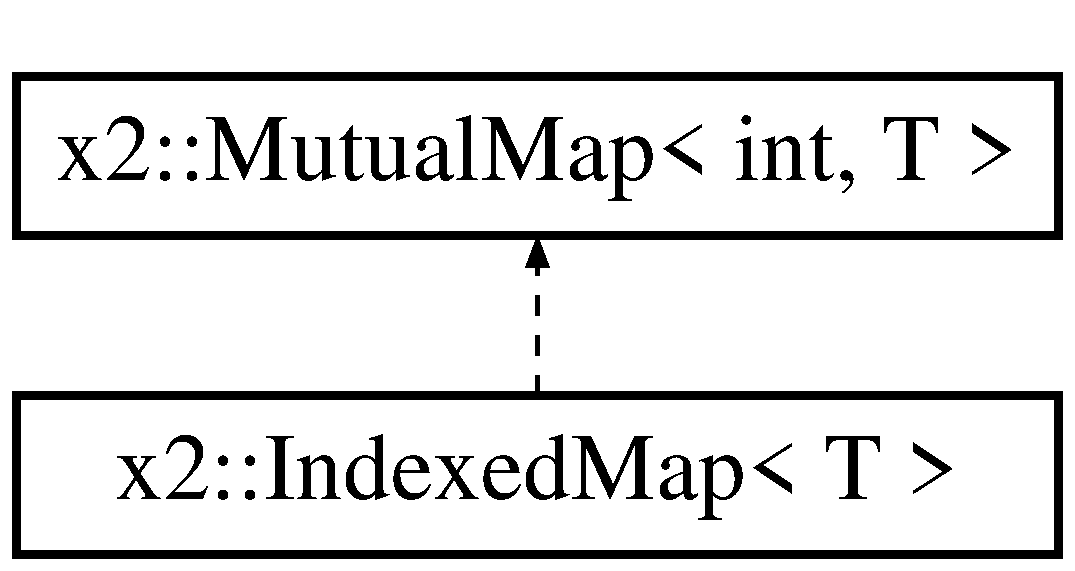
\includegraphics[height=2.000000cm]{classx2_1_1_indexed_map}
\end{center}
\end{figure}
\subsection*{Public Types}
\begin{DoxyCompactItemize}
\item 
\mbox{\Hypertarget{classx2_1_1_indexed_map_ac4647adcaec364cbcd569a83faabccfe}\label{classx2_1_1_indexed_map_ac4647adcaec364cbcd569a83faabccfe}} 
typedef \hyperlink{classx2_1_1_mutual_map}{Mutual\+Map}$<$ int, T $>$ {\bfseries Father}
\item 
\mbox{\Hypertarget{classx2_1_1_indexed_map_a9541095b80539c1deb7248b59a8adbdf}\label{classx2_1_1_indexed_map_a9541095b80539c1deb7248b59a8adbdf}} 
typedef \hyperlink{classx2_1_1_indexed_map}{Indexed\+Map} {\bfseries This}
\end{DoxyCompactItemize}
\subsection*{Public Member Functions}
\begin{DoxyCompactItemize}
\item 
\mbox{\Hypertarget{classx2_1_1_indexed_map_a0ae7462f1bfbc8145fa992cc0bfaa923}\label{classx2_1_1_indexed_map_a0ae7462f1bfbc8145fa992cc0bfaa923}} 
{\bfseries Indexed\+Map} (const \hyperlink{classx2_1_1_indexed_map}{Indexed\+Map}$<$ T $>$ \&map)=default
\item 
\mbox{\Hypertarget{classx2_1_1_indexed_map_ae77e782d05e1f99e84be949f0834c710}\label{classx2_1_1_indexed_map_ae77e782d05e1f99e84be949f0834c710}} 
{\bfseries Indexed\+Map} (\hyperlink{classx2_1_1_indexed_map}{Indexed\+Map}$<$ T $>$ \&\&map)=default
\item 
\mbox{\Hypertarget{classx2_1_1_indexed_map_aaab5c1c5eb826a61725e8527f8ad3aa0}\label{classx2_1_1_indexed_map_aaab5c1c5eb826a61725e8527f8ad3aa0}} 
{\bfseries Indexed\+Map} (const T \&failedT)
\item 
\mbox{\Hypertarget{classx2_1_1_indexed_map_a8973ed906cd8d78344139765cb8fe0c0}\label{classx2_1_1_indexed_map_a8973ed906cd8d78344139765cb8fe0c0}} 
{\bfseries Indexed\+Map} (const T \&failedT, std\+::initializer\+\_\+list$<$ T $>$ list)
\item 
\mbox{\Hypertarget{classx2_1_1_indexed_map_a8a13faf490943dc5b95bb55c90174aa1}\label{classx2_1_1_indexed_map_a8a13faf490943dc5b95bb55c90174aa1}} 
{\bfseries Indexed\+Map} (const T \&failedT, const std\+::vector$<$ T $>$ \&list)
\item 
\mbox{\Hypertarget{classx2_1_1_indexed_map_a953add6e946eccbe53a8cfb817ea06c7}\label{classx2_1_1_indexed_map_a953add6e946eccbe53a8cfb817ea06c7}} 
int {\bfseries get} (const T \&t) const
\item 
\mbox{\Hypertarget{classx2_1_1_indexed_map_aaddb767a7970a551177b8d8198603ac8}\label{classx2_1_1_indexed_map_aaddb767a7970a551177b8d8198603ac8}} 
const T \& {\bfseries get} (int i) const
\item 
\mbox{\Hypertarget{classx2_1_1_indexed_map_aa95f0065873bed75257da67c3111f75c}\label{classx2_1_1_indexed_map_aa95f0065873bed75257da67c3111f75c}} 
int {\bfseries get\+Add} (const T \&t)
\item 
\mbox{\Hypertarget{classx2_1_1_indexed_map_a8841875de3bb775a698377b5cb160fdd}\label{classx2_1_1_indexed_map_a8841875de3bb775a698377b5cb160fdd}} 
void {\bfseries set} (int i, const T \&t)
\item 
void \hyperlink{classx2_1_1_indexed_map_a76211a5e565fd668c39f00f2935d6481}{add} (const T \&t)
\item 
\mbox{\Hypertarget{classx2_1_1_indexed_map_a15516e7f6557faff0697a7ae9ce95e2a}\label{classx2_1_1_indexed_map_a15516e7f6557faff0697a7ae9ce95e2a}} 
void {\bfseries remove} (const T \&t)
\end{DoxyCompactItemize}
\subsection*{Protected Attributes}
\begin{DoxyCompactItemize}
\item 
\mbox{\Hypertarget{classx2_1_1_indexed_map_ab683c90c6f8eadc051bd74eadcb5b2b7}\label{classx2_1_1_indexed_map_ab683c90c6f8eadc051bd74eadcb5b2b7}} 
int {\bfseries max}
\end{DoxyCompactItemize}
\subsection*{Static Protected Attributes}
\begin{DoxyCompactItemize}
\item 
\mbox{\Hypertarget{classx2_1_1_indexed_map_acb56a512932a44a9f6e3245e283ec1a0}\label{classx2_1_1_indexed_map_acb56a512932a44a9f6e3245e283ec1a0}} 
static int {\bfseries U\+N\+D\+E\+F\+I\+N\+E\+D\+\_\+\+I\+N\+D\+EX} =-\/2
\end{DoxyCompactItemize}
\subsection*{Additional Inherited Members}


\subsection{Detailed Description}
\subsubsection*{template$<$class T$>$\newline
class x2\+::\+Indexed\+Map$<$ T $>$}

visit all through T,not by index 

\subsection{Member Function Documentation}
\mbox{\Hypertarget{classx2_1_1_indexed_map_a76211a5e565fd668c39f00f2935d6481}\label{classx2_1_1_indexed_map_a76211a5e565fd668c39f00f2935d6481}} 
\index{x2\+::\+Indexed\+Map@{x2\+::\+Indexed\+Map}!add@{add}}
\index{add@{add}!x2\+::\+Indexed\+Map@{x2\+::\+Indexed\+Map}}
\subsubsection{\texorpdfstring{add()}{add()}}
{\footnotesize\ttfamily template$<$class T$>$ \\
void \hyperlink{classx2_1_1_indexed_map}{x2\+::\+Indexed\+Map}$<$ T $>$\+::add (\begin{DoxyParamCaption}\item[{const T \&}]{t }\end{DoxyParamCaption})\hspace{0.3cm}{\ttfamily [inline]}}

always succeed 

The documentation for this class was generated from the following file\+:\begin{DoxyCompactItemize}
\item 
D\+:/\+Pool/eclipse-\/workspace/compiler-\/debug/include/Mutual\+Map.\+h\end{DoxyCompactItemize}

\hypertarget{classx2_1_1_indexed_map_3_01int_01_4}{}\section{x2\+:\+:Indexed\+Map$<$ int $>$ Class Template Reference}
\label{classx2_1_1_indexed_map_3_01int_01_4}\index{x2\+::\+Indexed\+Map$<$ int $>$@{x2\+::\+Indexed\+Map$<$ int $>$}}


{\ttfamily \#include $<$Mutual\+Map.\+h$>$}



\subsection{Detailed Description}
\subsubsection*{template$<$$>$\newline
class x2\+::\+Indexed\+Map$<$ int $>$}

the special type of int is not defined. 

The documentation for this class was generated from the following file\+:\begin{DoxyCompactItemize}
\item 
D\+:/\+Pool/eclipse-\/workspace/compiler-\/debug/include/Mutual\+Map.\+h\end{DoxyCompactItemize}

\hypertarget{classx2_1_1_lexical_output_stream_processor}{}\section{x2\+:\+:Lexical\+Output\+Stream\+Processor$<$ T, V $>$ Class Template Reference}
\label{classx2_1_1_lexical_output_stream_processor}\index{x2\+::\+Lexical\+Output\+Stream\+Processor$<$ T, V $>$@{x2\+::\+Lexical\+Output\+Stream\+Processor$<$ T, V $>$}}


{\ttfamily \#include $<$F\+A\+Utils.\+h$>$}

Inheritance diagram for x2\+:\+:Lexical\+Output\+Stream\+Processor$<$ T, V $>$\+:\begin{figure}[H]
\begin{center}
\leavevmode
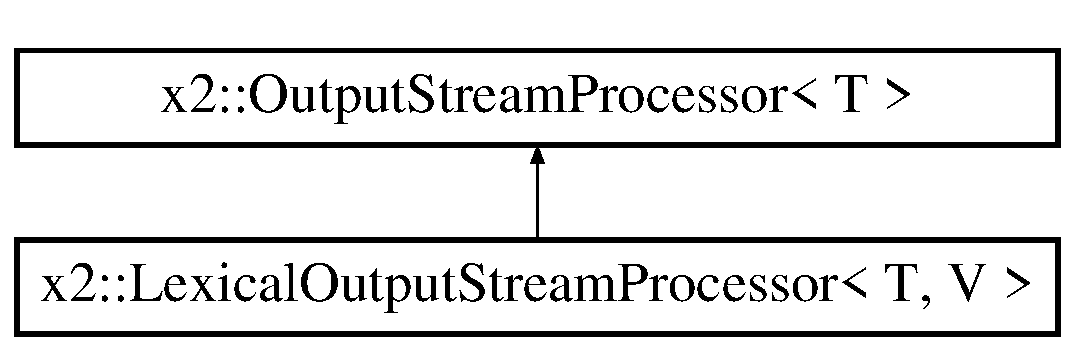
\includegraphics[height=2.000000cm]{classx2_1_1_lexical_output_stream_processor}
\end{center}
\end{figure}
\subsection*{Public Types}
\begin{DoxyCompactItemize}
\item 
enum \hyperlink{classx2_1_1_lexical_output_stream_processor_a221c7064aea399ed949761e3e784acd7}{P\+O\+S\+I\+T\+I\+O\+N\+\_\+\+A\+C\+T\+I\+ON} \{ {\bfseries P\+O\+S\+I\+T\+I\+O\+N\+\_\+\+A\+P\+P\+E\+ND} =0, 
{\bfseries P\+O\+S\+I\+T\+I\+O\+N\+\_\+\+N\+EW} =1, 
{\bfseries P\+O\+S\+I\+T\+I\+O\+N\+\_\+\+N\+E\+W\+A\+P\+P\+E\+ND} =2, 
{\bfseries P\+O\+S\+I\+T\+I\+O\+N\+\_\+\+I\+G\+N\+O\+RE} =3
 \}
\item 
\mbox{\Hypertarget{classx2_1_1_lexical_output_stream_processor_af5c4b994e1ac814f7c39d21e0caa8375}\label{classx2_1_1_lexical_output_stream_processor_af5c4b994e1ac814f7c39d21e0caa8375}} 
typedef std\+::vector$<$ std\+::pair$<$ V, int $>$ $>$ {\bfseries Output\+Stream\+Type}
\item 
\mbox{\Hypertarget{classx2_1_1_lexical_output_stream_processor_a9db9908c3ea85542720488129efc4245}\label{classx2_1_1_lexical_output_stream_processor_a9db9908c3ea85542720488129efc4245}} 
typedef std\+::map$<$ std\+::pair$<$ int, int $>$, std\+::pair$<$ int, int $>$ $>$ {\bfseries Action\+Type}
\end{DoxyCompactItemize}
\subsection*{Public Member Functions}
\begin{DoxyCompactItemize}
\item 
\mbox{\Hypertarget{classx2_1_1_lexical_output_stream_processor_a3c6459aa48678f1f021c2173949b1da8}\label{classx2_1_1_lexical_output_stream_processor_a3c6459aa48678f1f021c2173949b1da8}} 
{\bfseries Lexical\+Output\+Stream\+Processor} (\hyperlink{classx2_1_1_finite_automata}{Finite\+Automata}$<$ T $>$ \&da)
\item 
\mbox{\Hypertarget{classx2_1_1_lexical_output_stream_processor_a776187b870429aec3d29639cfec125cb}\label{classx2_1_1_lexical_output_stream_processor_a776187b870429aec3d29639cfec125cb}} 
Output\+Stream\+Type \& {\bfseries get\+Cached\+Stream} ()
\item 
\mbox{\Hypertarget{classx2_1_1_lexical_output_stream_processor_a604f90577a9a2edb5a46d48e23bdbe3f}\label{classx2_1_1_lexical_output_stream_processor_a604f90577a9a2edb5a46d48e23bdbe3f}} 
const Output\+Stream\+Type \& {\bfseries get\+Cached\+Stream} () const
\item 
\mbox{\Hypertarget{classx2_1_1_lexical_output_stream_processor_af48a62609df67717be94c7d9bb979807}\label{classx2_1_1_lexical_output_stream_processor_af48a62609df67717be94c7d9bb979807}} 
virtual void {\bfseries process} (int cur\+State, const T \&in)
\item 
\mbox{\Hypertarget{classx2_1_1_lexical_output_stream_processor_a4733c0d4578dbce6e87804fbe7db327e}\label{classx2_1_1_lexical_output_stream_processor_a4733c0d4578dbce6e87804fbe7db327e}} 
void {\bfseries add\+Type} (std\+::pair$<$ std\+::string, T $>$ key, std\+::pair$<$ std\+::string, int $>$ value)
\item 
\mbox{\Hypertarget{classx2_1_1_lexical_output_stream_processor_a7e25ccd87f2694194cb28545194ccd1c}\label{classx2_1_1_lexical_output_stream_processor_a7e25ccd87f2694194cb28545194ccd1c}} 
void {\bfseries add\+Type} (std\+::pair$<$ int, int $>$ key, std\+::pair$<$ int, int $>$ value)
\end{DoxyCompactItemize}
\subsection*{Protected Attributes}
\begin{DoxyCompactItemize}
\item 
\mbox{\Hypertarget{classx2_1_1_lexical_output_stream_processor_a26c478133a4944e7eb19872d6ca78eba}\label{classx2_1_1_lexical_output_stream_processor_a26c478133a4944e7eb19872d6ca78eba}} 
\hyperlink{classx2_1_1_finite_automata}{Finite\+Automata}$<$ T $>$ \& {\bfseries fa}
\item 
\mbox{\Hypertarget{classx2_1_1_lexical_output_stream_processor_a255e05cf7a51dc60d2b7afe02ff4eec6}\label{classx2_1_1_lexical_output_stream_processor_a255e05cf7a51dc60d2b7afe02ff4eec6}} 
Output\+Stream\+Type {\bfseries cached\+Stream}
\item 
\mbox{\Hypertarget{classx2_1_1_lexical_output_stream_processor_a54670c34772bcf9763f45065d7564d52}\label{classx2_1_1_lexical_output_stream_processor_a54670c34772bcf9763f45065d7564d52}} 
Action\+Type {\bfseries actions}
\item 
\mbox{\Hypertarget{classx2_1_1_lexical_output_stream_processor_a79c52ead270f8e1b6c2ed44a362c4267}\label{classx2_1_1_lexical_output_stream_processor_a79c52ead270f8e1b6c2ed44a362c4267}} 
\hyperlink{classx2_1_1_indexed_map}{Indexed\+Map}$<$ std\+::string $>$ {\bfseries type\+Info}
\end{DoxyCompactItemize}


\subsection{Detailed Description}
\subsubsection*{template$<$class T, class V$>$\newline
class x2\+::\+Lexical\+Output\+Stream\+Processor$<$ T, V $>$}

一般的词法分析器要求输出 $<$ 值,类型$>$=\char`\"{}\char`\"{}$>$两种 有些值,比如int,类型是\+I\+D,\+I\+D-\/int就可以作为一种语法引导符号 V is a vector-\/like container V supports\+: constructs from \{\} push\+\_\+back(\+T) 

\subsection{Member Enumeration Documentation}
\mbox{\Hypertarget{classx2_1_1_lexical_output_stream_processor_a221c7064aea399ed949761e3e784acd7}\label{classx2_1_1_lexical_output_stream_processor_a221c7064aea399ed949761e3e784acd7}} 
\index{x2\+::\+Lexical\+Output\+Stream\+Processor@{x2\+::\+Lexical\+Output\+Stream\+Processor}!P\+O\+S\+I\+T\+I\+O\+N\+\_\+\+A\+C\+T\+I\+ON@{P\+O\+S\+I\+T\+I\+O\+N\+\_\+\+A\+C\+T\+I\+ON}}
\index{P\+O\+S\+I\+T\+I\+O\+N\+\_\+\+A\+C\+T\+I\+ON@{P\+O\+S\+I\+T\+I\+O\+N\+\_\+\+A\+C\+T\+I\+ON}!x2\+::\+Lexical\+Output\+Stream\+Processor@{x2\+::\+Lexical\+Output\+Stream\+Processor}}
\subsubsection{\texorpdfstring{P\+O\+S\+I\+T\+I\+O\+N\+\_\+\+A\+C\+T\+I\+ON}{POSITION\_ACTION}}
{\footnotesize\ttfamily template$<$class T, class V$>$ \\
enum \hyperlink{classx2_1_1_lexical_output_stream_processor_a221c7064aea399ed949761e3e784acd7}{x2\+::\+Lexical\+Output\+Stream\+Processor\+::\+P\+O\+S\+I\+T\+I\+O\+N\+\_\+\+A\+C\+T\+I\+ON}}

position = new or keep 

The documentation for this class was generated from the following file\+:\begin{DoxyCompactItemize}
\item 
D\+:/\+Pool/eclipse-\/workspace/compiler-\/debug/include/F\+A\+Utils.\+h\end{DoxyCompactItemize}

\hypertarget{classx2_1_1_lexical_parser}{}\section{x2\+:\+:Lexical\+Parser Class Reference}
\label{classx2_1_1_lexical_parser}\index{x2\+::\+Lexical\+Parser@{x2\+::\+Lexical\+Parser}}
\subsection*{Public Types}
\begin{DoxyCompactItemize}
\item 
\mbox{\Hypertarget{classx2_1_1_lexical_parser_a0349435d24793ac365f23265c9ef49f1}\label{classx2_1_1_lexical_parser_a0349435d24793ac365f23265c9ef49f1}} 
enum \{ \newline
{\bfseries S\+T\+A\+T\+E\+\_\+\+S\+T\+A\+RT}, 
{\bfseries S\+T\+A\+T\+E\+\_\+\+L\+E\+SS}, 
{\bfseries S\+T\+A\+T\+E\+\_\+\+G\+R\+E\+A\+T\+ER}, 
{\bfseries S\+T\+A\+T\+E\+\_\+\+D\+O\+U\+B\+L\+E\+\_\+\+G\+R\+E\+A\+T\+ER}, 
\newline
{\bfseries S\+T\+A\+T\+E\+\_\+\+E\+Q\+U\+AL}, 
{\bfseries S\+T\+A\+T\+E\+\_\+\+D\+I\+V\+ID}, 
{\bfseries S\+T\+A\+T\+E\+\_\+\+S\+T\+AR}, 
{\bfseries S\+T\+A\+T\+E\+\_\+\+N\+O\+TE}, 
\newline
{\bfseries S\+T\+A\+T\+E\+\_\+\+L\+I\+N\+E\+\_\+\+N\+O\+TE}, 
{\bfseries S\+T\+A\+T\+E\+\_\+\+M\+U\+L\+T\+I\+L\+I\+N\+E\+\_\+\+N\+O\+TE}, 
{\bfseries S\+T\+A\+T\+E\+\_\+\+M\+U\+L\+T\+I\+L\+I\+N\+E\+\_\+\+G\+O\+I\+N\+G\+\_\+\+E\+ND}, 
{\bfseries S\+T\+A\+T\+E\+\_\+\+T\+R\+A\+N\+S\+F\+E\+R\+\_\+\+C\+O\+M\+M\+ON}, 
\newline
{\bfseries S\+T\+A\+T\+E\+\_\+\+T\+R\+A\+N\+S\+F\+E\+R\+\_\+\+C\+O\+M\+M\+O\+N\+\_\+\+X1}, 
{\bfseries S\+T\+A\+T\+E\+\_\+\+T\+R\+A\+N\+S\+F\+E\+R\+\_\+\+C\+O\+M\+M\+O\+N\+\_\+\+X2}, 
{\bfseries S\+T\+A\+T\+E\+\_\+\+T\+R\+A\+N\+S\+F\+E\+R\+\_\+\+C\+O\+M\+M\+O\+N\+\_\+\+U1}, 
{\bfseries S\+T\+A\+T\+E\+\_\+\+T\+R\+A\+N\+S\+F\+E\+R\+\_\+\+C\+A\+R\+R\+I\+GE}, 
\newline
{\bfseries S\+T\+A\+T\+E\+\_\+\+T\+R\+A\+N\+S\+F\+E\+R\+\_\+\+L\+A\+N\+G\+U\+A\+GE}, 
{\bfseries S\+T\+A\+T\+E\+\_\+\+T\+R\+A\+N\+S\+F\+E\+R\+\_\+\+C\+H\+AR}, 
{\bfseries S\+T\+A\+T\+E\+\_\+\+T\+R\+A\+N\+S\+F\+E\+R\+\_\+\+S\+T\+R\+I\+NG}, 
{\bfseries S\+T\+A\+T\+E\+\_\+\+T\+R\+A\+N\+S\+F\+E\+R\+\_\+\+V\+A\+L\+UE}, 
\newline
{\bfseries S\+T\+A\+T\+E\+\_\+\+ID}, 
{\bfseries S\+T\+A\+T\+E\+\_\+\+K\+E\+E\+P\+\_\+\+S\+P\+A\+CE}, 
{\bfseries S\+T\+A\+T\+E\+\_\+\+S\+T\+R\+I\+NG}, 
{\bfseries S\+T\+A\+T\+E\+\_\+\+C\+H\+AR}, 
\newline
{\bfseries S\+T\+A\+T\+E\+\_\+\+N\+U\+M\+B\+ER}, 
{\bfseries S\+T\+A\+T\+E\+\_\+\+H\+E\+X\+\_\+\+N\+U\+M\+B\+ER}, 
{\bfseries S\+T\+A\+T\+E\+\_\+\+D\+E\+C\+I\+L\+M\+A\+L\+\_\+\+N\+U\+M\+B\+ER}, 
{\bfseries S\+T\+A\+T\+E\+\_\+\+B\+I\+N\+\_\+\+N\+U\+M\+B\+ER}, 
\newline
{\bfseries S\+T\+A\+T\+E\+\_\+\+N\+O\+\_\+\+C\+A\+RE}, 
{\bfseries S\+T\+A\+T\+E\+\_\+\+E\+ND}, 
{\bfseries S\+T\+A\+T\+E\+\_\+\+U\+N\+R\+E\+C\+O\+G\+N\+I\+Z\+E\+D\+\_\+\+C\+H\+AR}, 
{\bfseries S\+T\+A\+T\+E\+\_\+\+T\+R\+A\+N\+S\+F\+E\+R\+\_\+\+H\+E\+X\+\_\+\+N\+O\+T\+\_\+\+E\+N\+O\+G\+UH}, 
\newline
{\bfseries S\+T\+A\+T\+E\+\_\+\+T\+R\+A\+N\+S\+F\+E\+R\+\_\+\+I\+N\+V\+A\+L\+ID}, 
{\bfseries S\+T\+A\+T\+E\+\_\+\+L\+A\+ST}
 \}
\item 
\mbox{\Hypertarget{classx2_1_1_lexical_parser_ac5ee05b7590effdd000a1ea82e16fe35}\label{classx2_1_1_lexical_parser_ac5ee05b7590effdd000a1ea82e16fe35}} 
enum \{ {\bfseries D\+O\+N\+E\+\_\+\+O\+N\+E\+\_\+\+W\+O\+RD}, 
{\bfseries D\+O\+I\+N\+G\+\_\+\+O\+N\+E\+\_\+\+W\+R\+OD}
 \}
\item 
\mbox{\Hypertarget{classx2_1_1_lexical_parser_a74d54e4dc992530d4bcd4aab4c8da6f8}\label{classx2_1_1_lexical_parser_a74d54e4dc992530d4bcd4aab4c8da6f8}} 
enum \{ \newline
{\bfseries T\+Y\+P\+E\+\_\+\+OP} =0, 
{\bfseries T\+Y\+P\+E\+\_\+\+S\+E\+M\+I\+C\+O\+L\+ON} =1, 
{\bfseries T\+Y\+P\+E\+\_\+\+S\+I\+N\+G\+LE} =44, 
{\bfseries T\+Y\+P\+E\+\_\+\+EQ} =26, 
\newline
{\bfseries T\+Y\+P\+E\+\_\+\+D\+IV}, 
{\bfseries T\+Y\+P\+E\+\_\+\+P\+L\+US}, 
{\bfseries T\+Y\+P\+E\+\_\+\+A\+ND}, 
{\bfseries T\+Y\+P\+E\+\_\+\+E\+XP}, 
\newline
{\bfseries T\+Y\+P\+E\+\_\+\+M\+OD}, 
{\bfseries T\+Y\+P\+E\+\_\+\+D\+O\+L\+L\+AR}, 
{\bfseries T\+Y\+P\+E\+\_\+\+N\+OT}, 
{\bfseries T\+Y\+P\+E\+\_\+\+S\+UB}, 
\newline
{\bfseries T\+Y\+P\+E\+\_\+\+C\+O\+M\+MA}, 
{\bfseries T\+Y\+P\+E\+\_\+\+W\+A\+VE}, 
{\bfseries T\+Y\+P\+E\+\_\+\+R\+Q\+U\+O\+TE}, 
{\bfseries T\+Y\+P\+E\+\_\+\+C\+O\+L\+ON}, 
\newline
{\bfseries T\+Y\+P\+E\+\_\+\+E\+R\+E\+CT}, 
{\bfseries T\+Y\+P\+E\+\_\+\+A\+SK}, 
{\bfseries T\+Y\+P\+E\+\_\+\+P\+O\+I\+NT}, 
{\bfseries T\+Y\+P\+E\+\_\+\+U\+N\+D\+E\+R\+S\+C\+O\+RE} =48, 
\newline
{\bfseries T\+Y\+P\+E\+\_\+\+L\+SQ}, 
{\bfseries T\+Y\+P\+E\+\_\+\+R\+SQ}, 
{\bfseries T\+Y\+P\+E\+\_\+\+AT}, 
{\bfseries T\+Y\+P\+E\+\_\+\+Q\+U\+O\+TE}, 
\newline
{\bfseries T\+Y\+P\+E\+\_\+\+D\+Q\+U\+O\+TE} =53, 
{\bfseries T\+Y\+P\+E\+\_\+\+N\+U\+M\+B\+E\+R\+\_\+\+D\+E\+C\+I\+M\+AL} =2, 
{\bfseries T\+Y\+P\+E\+\_\+\+N\+U\+M\+B\+E\+R\+\_\+\+B\+IN} =23, 
{\bfseries T\+Y\+P\+E\+\_\+\+N\+U\+M\+B\+E\+R\+\_\+\+H\+EX} =24, 
\newline
{\bfseries T\+Y\+P\+E\+\_\+\+ID} =3, 
{\bfseries T\+Y\+P\+E\+\_\+\+S\+T\+R\+I\+NG} =4, 
{\bfseries T\+Y\+P\+E\+\_\+\+C\+H\+AR} =5, 
{\bfseries T\+Y\+P\+E\+\_\+\+T\+R\+A\+N\+S\+F\+ER} =6, 
\newline
{\bfseries T\+Y\+P\+E\+\_\+\+S1} =16, 
{\bfseries T\+Y\+P\+E\+\_\+\+N\+E\+W\+L\+I\+NE} =7, 
{\bfseries T\+Y\+P\+E\+\_\+\+L\+E\+SS} =17, 
{\bfseries T\+Y\+P\+E\+\_\+\+G\+R\+E\+A\+T\+ER} =18, 
\newline
{\bfseries T\+Y\+P\+E\+\_\+\+N\+O\+TE} =8, 
{\bfseries T\+Y\+P\+E\+\_\+\+I\+N\+L\+I\+N\+E\+\_\+\+N\+O\+TE} =55, 
{\bfseries T\+Y\+P\+E\+\_\+\+F\+R\+E\+E\+\_\+\+N\+O\+TE}, 
{\bfseries T\+Y\+P\+E\+\_\+\+D\+O\+C\+\_\+\+N\+O\+TE} =57, 
\newline
{\bfseries T\+Y\+P\+E\+\_\+\+L\+B\+R\+A\+CE} =9, 
{\bfseries T\+Y\+P\+E\+\_\+\+R\+B\+R\+A\+CE} =10, 
{\bfseries T\+Y\+P\+E\+\_\+\+L\+H\+B\+R\+A\+CE} =11, 
{\bfseries T\+Y\+P\+E\+\_\+\+R\+H\+B\+R\+A\+CE} =12, 
\newline
{\bfseries T\+Y\+P\+E\+\_\+\+S\+T\+AR} =13, 
{\bfseries T\+Y\+P\+E\+\_\+\+N\+O\+NE} =14, 
{\bfseries T\+Y\+P\+E\+\_\+\+U\+N\+K\+N\+OW} =15, 
{\bfseries T\+Y\+P\+E\+\_\+\+E\+R\+R\+OR} =25, 
\newline
{\bfseries T\+Y\+P\+E\+\_\+\+U\+N\+R\+E\+C\+O\+G\+N\+I\+Z\+ED} =43, 
{\bfseries T\+Y\+P\+E\+\_\+\+S\+P\+A\+CE} =45, 
{\bfseries T\+Y\+P\+E\+\_\+\+E\+ND} =46, 
{\bfseries T\+Y\+P\+E\+\_\+\+I\+N\+F\+O\+\_\+\+L\+O\+ST} =47, 
\newline
{\bfseries T\+Y\+P\+E\+\_\+\+L\+A\+ST} =54
 \}
\item 
\mbox{\Hypertarget{classx2_1_1_lexical_parser_a7bed4bbbaccf1d7d64acefd646ac3fca}\label{classx2_1_1_lexical_parser_a7bed4bbbaccf1d7d64acefd646ac3fca}} 
enum \{ \newline
{\bfseries D\+I\+G\+I\+T\+\_\+\+B\+IN} =0, 
{\bfseries D\+I\+G\+I\+T\+\_\+\+D\+E\+C\+I\+M\+AL}, 
{\bfseries D\+I\+G\+I\+T\+\_\+\+H\+E\+X\+\_\+\+L\+O\+W\+ER}, 
{\bfseries D\+I\+G\+I\+T\+\_\+\+H\+E\+X\+\_\+\+U\+P\+P\+ER}, 
\newline
{\bfseries D\+I\+G\+I\+T\+\_\+\+U\+N\+K\+N\+O\+WN}
 \}
\item 
\mbox{\Hypertarget{classx2_1_1_lexical_parser_ab9bf3af0acdca4958080513ae4bffb2e}\label{classx2_1_1_lexical_parser_ab9bf3af0acdca4958080513ae4bffb2e}} 
enum \{ \newline
{\bfseries S\+E\+T\+\_\+\+A\+L\+P\+HA}, 
{\bfseries S\+E\+T\+\_\+\+W\+O\+RD}, 
{\bfseries S\+E\+T\+\_\+\+B\+IN}, 
{\bfseries S\+E\+T\+\_\+\+D\+EC}, 
\newline
{\bfseries S\+E\+T\+\_\+\+H\+EX}, 
{\bfseries S\+E\+T\+\_\+\+S\+P\+A\+CE}, 
{\bfseries S\+E\+T\+\_\+\+S\+P\+E\+C\+I\+AL}, 
{\bfseries S\+E\+T\+\_\+\+S\+I\+ZE}
 \}
\item 
\mbox{\Hypertarget{classx2_1_1_lexical_parser_a2888218380e69d89c1e05ff4b6080aa6}\label{classx2_1_1_lexical_parser_a2888218380e69d89c1e05ff4b6080aa6}} 
typedef \hyperlink{classx2_1_1_lexical_parser}{Lexical\+Parser} {\bfseries This}
\item 
\mbox{\Hypertarget{classx2_1_1_lexical_parser_a6b384459924122c338c117307e0a90f8}\label{classx2_1_1_lexical_parser_a6b384459924122c338c117307e0a90f8}} 
typedef bool($\ast$ {\bfseries J\+U\+D\+G\+E\+\_\+\+C\+H\+AR}) (char ch)
\item 
\mbox{\Hypertarget{classx2_1_1_lexical_parser_aaf7b341c51dcd3f1bfe0773e68c91209}\label{classx2_1_1_lexical_parser_aaf7b341c51dcd3f1bfe0773e68c91209}} 
typedef std\+::map$<$ int, std\+::string $>$ {\bfseries Trans\+Map}
\item 
\mbox{\Hypertarget{classx2_1_1_lexical_parser_a1b56b8aa6baecaa64fa6d1d0992d89f1}\label{classx2_1_1_lexical_parser_a1b56b8aa6baecaa64fa6d1d0992d89f1}} 
typedef std\+::map$<$ char, int $>$ {\bfseries Char\+Type}
\item 
\mbox{\Hypertarget{classx2_1_1_lexical_parser_aa46a59aa1c34176e923676c9518f5f75}\label{classx2_1_1_lexical_parser_aa46a59aa1c34176e923676c9518f5f75}} 
using {\bfseries Word\+Stream} = typename Lexical\+To\+Grammar\+Stream\+::\+Word\+Stream
\end{DoxyCompactItemize}
\subsection*{Public Member Functions}
\begin{DoxyCompactItemize}
\item 
void \hyperlink{classx2_1_1_lexical_parser_ad145a31ea89f2c203bb894226f37c424}{parse\+Number} (const char $\ast$buffer, size\+\_\+t len)=delete
\item 
\mbox{\Hypertarget{classx2_1_1_lexical_parser_a66dd4881cb37ca304b2431e9cf9f7c2f}\label{classx2_1_1_lexical_parser_a66dd4881cb37ca304b2431e9cf9f7c2f}} 
void {\bfseries parse\+String} (const char $\ast$buffer, size\+\_\+t \&index, size\+\_\+t len)=delete
\item 
Word\+Stream \hyperlink{classx2_1_1_lexical_parser_ae60c0630386d1f6619fb2ba82955934e}{parse\+Words} (std\+::istream \&in)
\item 
\mbox{\Hypertarget{classx2_1_1_lexical_parser_a4a3bee404dceece2ca0bfec782d8561b}\label{classx2_1_1_lexical_parser_a4a3bee404dceece2ca0bfec782d8561b}} 
void {\bfseries parse\+Preps} (const char $\ast$buffer, size\+\_\+t \&index, size\+\_\+t len)=delete
\item 
\mbox{\Hypertarget{classx2_1_1_lexical_parser_ac6dd1193fa3a1c493a20143196749e3b}\label{classx2_1_1_lexical_parser_ac6dd1193fa3a1c493a20143196749e3b}} 
void {\bfseries parse\+Id} (const char $\ast$buffer, size\+\_\+t \&index, size\+\_\+t len, std\+::string \&out, int \&type)=delete
\item 
\mbox{\Hypertarget{classx2_1_1_lexical_parser_a6ef3f63cce691e5f7286988b843dfe27}\label{classx2_1_1_lexical_parser_a6ef3f63cce691e5f7286988b843dfe27}} 
void {\bfseries parse\+Number} (const char $\ast$buffer, size\+\_\+t \&index, size\+\_\+t len, std\+::string \&out, int \&type)=delete
\item 
void \hyperlink{classx2_1_1_lexical_parser_a0cf09764367aa7e6ccf044150bb9d435}{parse\+Transfer\+Id} (const char $\ast$buffer, size\+\_\+t \&index, size\+\_\+t len, std\+::string \&out, int \&type)=delete
\item 
void \hyperlink{classx2_1_1_lexical_parser_a719a5e77295d26d71de8381757fc1ab5}{parse\+Transfer\+Value} (const char $\ast$buffer, size\+\_\+t \&index, size\+\_\+t len, std\+::string \&out, int \&type)=delete
\item 
\mbox{\Hypertarget{classx2_1_1_lexical_parser_a56b78c6b78c71f94ed399a0237f452cc}\label{classx2_1_1_lexical_parser_a56b78c6b78c71f94ed399a0237f452cc}} 
void {\bfseries parse\+Transfer\+Any} (const char $\ast$buffer, size\+\_\+t \&index, size\+\_\+t len, std\+::string \&out, int \&type)=delete
\item 
\mbox{\Hypertarget{classx2_1_1_lexical_parser_a114cc369f550f24b5b5a06ba1b622347}\label{classx2_1_1_lexical_parser_a114cc369f550f24b5b5a06ba1b622347}} 
void {\bfseries parse\+String} (const char $\ast$buffer, size\+\_\+t \&index, size\+\_\+t len, std\+::string \&out, int \&type)=delete
\item 
\mbox{\Hypertarget{classx2_1_1_lexical_parser_a5955d1d987c91e7620ac06548f37a53c}\label{classx2_1_1_lexical_parser_a5955d1d987c91e7620ac06548f37a53c}} 
void {\bfseries parse\+Note} (const char $\ast$buffer, size\+\_\+t \&index, size\+\_\+t len, std\+::string \&out, int \&type)=delete
\item 
\mbox{\Hypertarget{classx2_1_1_lexical_parser_a79e43313b550c378106a04017c92b54d}\label{classx2_1_1_lexical_parser_a79e43313b550c378106a04017c92b54d}} 
A\+S\+\_\+\+M\+A\+C\+RO void {\bfseries skip\+Spaces} (const char $\ast$buffer, size\+\_\+t \&index, size\+\_\+t len)=delete
\item 
void \hyperlink{classx2_1_1_lexical_parser_aa3c5fdf7dcce41c49671b5361992dc83}{error} (const char $\ast$msg) const
\end{DoxyCompactItemize}
\subsection*{Static Public Member Functions}
\begin{DoxyCompactItemize}
\item 
\mbox{\Hypertarget{classx2_1_1_lexical_parser_af29705ffe052b5677961178322ec9805}\label{classx2_1_1_lexical_parser_af29705ffe052b5677961178322ec9805}} 
static bool {\bfseries is\+Digit\+Type} (char ch, int type)
\item 
\mbox{\Hypertarget{classx2_1_1_lexical_parser_ab3be33ec664da5c1ec0eb0316b405be0}\label{classx2_1_1_lexical_parser_ab3be33ec664da5c1ec0eb0316b405be0}} 
static int {\bfseries tell\+Digit\+Type} (char ch)
\item 
\mbox{\Hypertarget{classx2_1_1_lexical_parser_a3d83db1d9a2f0438f2f35a60bea4dac7}\label{classx2_1_1_lexical_parser_a3d83db1d9a2f0438f2f35a60bea4dac7}} 
static bool {\bfseries is\+In\+Set} (char ch, const char $\ast$buffer, size\+\_\+t len)
\item 
\mbox{\Hypertarget{classx2_1_1_lexical_parser_a92a66e39a85bbabef3799ae21bc9fbcf}\label{classx2_1_1_lexical_parser_a92a66e39a85bbabef3799ae21bc9fbcf}} 
static A\+S\+\_\+\+M\+A\+C\+RO bool {\bfseries is\+In\+Set} (char ch, int set)
\item 
\mbox{\Hypertarget{classx2_1_1_lexical_parser_a05c3c1652ed12825a8b9da344abcb824}\label{classx2_1_1_lexical_parser_a05c3c1652ed12825a8b9da344abcb824}} 
static A\+S\+\_\+\+M\+A\+C\+RO bool {\bfseries is\+In\+Alpha} (char ch)
\item 
\mbox{\Hypertarget{classx2_1_1_lexical_parser_a642ff181c1c56cccb7015c24a6941c60}\label{classx2_1_1_lexical_parser_a642ff181c1c56cccb7015c24a6941c60}} 
static A\+S\+\_\+\+M\+A\+C\+RO bool {\bfseries is\+In\+Word} (char ch)
\item 
\mbox{\Hypertarget{classx2_1_1_lexical_parser_a5a8bb34203443bd5b3008f671da5fa98}\label{classx2_1_1_lexical_parser_a5a8bb34203443bd5b3008f671da5fa98}} 
static A\+S\+\_\+\+M\+A\+C\+RO bool {\bfseries is\+In\+Bin} (char ch)
\item 
\mbox{\Hypertarget{classx2_1_1_lexical_parser_ae53f57b10f1a677f4fe0244557c346f5}\label{classx2_1_1_lexical_parser_ae53f57b10f1a677f4fe0244557c346f5}} 
static A\+S\+\_\+\+M\+A\+C\+RO bool {\bfseries is\+In\+Dec} (char ch)
\item 
\mbox{\Hypertarget{classx2_1_1_lexical_parser_af15a122be3aae416676f721c5bc109f2}\label{classx2_1_1_lexical_parser_af15a122be3aae416676f721c5bc109f2}} 
static A\+S\+\_\+\+M\+A\+C\+RO bool {\bfseries is\+In\+Hex} (char ch)
\item 
\mbox{\Hypertarget{classx2_1_1_lexical_parser_a21b917a42d6b2b0d78c4b352c15c613a}\label{classx2_1_1_lexical_parser_a21b917a42d6b2b0d78c4b352c15c613a}} 
static A\+S\+\_\+\+M\+A\+C\+RO bool {\bfseries is\+In\+Space} (char ch)
\item 
\mbox{\Hypertarget{classx2_1_1_lexical_parser_a48591265bb5f4e634836004dd6ad676b}\label{classx2_1_1_lexical_parser_a48591265bb5f4e634836004dd6ad676b}} 
static A\+S\+\_\+\+M\+A\+C\+RO bool {\bfseries is\+In\+Special} (char ch)
\item 
\mbox{\Hypertarget{classx2_1_1_lexical_parser_a3014eaa73730e85c02e927c4485a0a68}\label{classx2_1_1_lexical_parser_a3014eaa73730e85c02e927c4485a0a68}} 
static A\+S\+\_\+\+M\+A\+C\+RO int {\bfseries get\+Special\+Type} (char ch)
\item 
\mbox{\Hypertarget{classx2_1_1_lexical_parser_ac7526de6db8cfdda58be67b824add45e}\label{classx2_1_1_lexical_parser_ac7526de6db8cfdda58be67b824add45e}} 
static A\+S\+\_\+\+M\+A\+C\+RO int {\bfseries get\+Char\+Val} (char ch)
\item 
\mbox{\Hypertarget{classx2_1_1_lexical_parser_a21f8b212b6564855027f8cf9dd854865}\label{classx2_1_1_lexical_parser_a21f8b212b6564855027f8cf9dd854865}} 
static A\+S\+\_\+\+M\+A\+C\+RO int {\bfseries get\+Char\+Val} (const char $\ast$str)=delete
\item 
\mbox{\Hypertarget{classx2_1_1_lexical_parser_a46d98ddbba0efcabf89b41d4aab6a6b3}\label{classx2_1_1_lexical_parser_a46d98ddbba0efcabf89b41d4aab6a6b3}} 
static int {\bfseries eval\+String} (const std\+::string \&s, int type=T\+Y\+P\+E\+\_\+\+N\+U\+M\+B\+E\+R\+\_\+\+D\+E\+C\+I\+M\+AL)=delete
\item 
\mbox{\Hypertarget{classx2_1_1_lexical_parser_a27e165dff3124bf6015be17b7867af82}\label{classx2_1_1_lexical_parser_a27e165dff3124bf6015be17b7867af82}} 
static int {\bfseries eval\+String} (const char $\ast$buffer, size\+\_\+t len, int type=T\+Y\+P\+E\+\_\+\+N\+U\+M\+B\+E\+R\+\_\+\+D\+E\+C\+I\+M\+AL)=delete
\item 
\mbox{\Hypertarget{classx2_1_1_lexical_parser_a71ee68324ef9653396de116d27fe1668}\label{classx2_1_1_lexical_parser_a71ee68324ef9653396de116d27fe1668}} 
static A\+S\+\_\+\+M\+A\+C\+RO const Trans\+Map \& {\bfseries get\+Human\+Readable} ()
\item 
\mbox{\Hypertarget{classx2_1_1_lexical_parser_a90afc8ede198df40426d1ffa0b35b44c}\label{classx2_1_1_lexical_parser_a90afc8ede198df40426d1ffa0b35b44c}} 
static A\+S\+\_\+\+M\+A\+C\+RO bool {\bfseries register\+Type\+String} (int type, const std\+::string \&s)
\item 
\mbox{\Hypertarget{classx2_1_1_lexical_parser_a3e83cdbdab47e6d58d19e3b43cd4da10}\label{classx2_1_1_lexical_parser_a3e83cdbdab47e6d58d19e3b43cd4da10}} 
static A\+S\+\_\+\+M\+A\+C\+RO const std\+::string \& {\bfseries get\+Type\+String} (int type)
\item 
\mbox{\Hypertarget{classx2_1_1_lexical_parser_a08b01efd66c599dd753673852ad21b89}\label{classx2_1_1_lexical_parser_a08b01efd66c599dd753673852ad21b89}} 
static char {\bfseries find\+Value} (char key, const char $\ast$buffer, size\+\_\+t len)
\end{DoxyCompactItemize}
\subsection*{Static Public Attributes}
\begin{DoxyCompactItemize}
\item 
static const J\+U\+D\+G\+E\+\_\+\+C\+H\+AR {\bfseries judge\+Arr} \mbox{[}S\+E\+T\+\_\+\+S\+I\+ZE\mbox{]}
\item 
\mbox{\Hypertarget{classx2_1_1_lexical_parser_a35fe61724b0957fe7e7fc059aa3f9748}\label{classx2_1_1_lexical_parser_a35fe61724b0957fe7e7fc059aa3f9748}} 
static Trans\+Map {\bfseries human\+Info}
\item 
\mbox{\Hypertarget{classx2_1_1_lexical_parser_a974b8f9c02b101ed6c5e58ec3be0b845}\label{classx2_1_1_lexical_parser_a974b8f9c02b101ed6c5e58ec3be0b845}} 
static Char\+Type {\bfseries char\+Type}
\end{DoxyCompactItemize}


\subsection{Member Function Documentation}
\mbox{\Hypertarget{classx2_1_1_lexical_parser_aa3c5fdf7dcce41c49671b5361992dc83}\label{classx2_1_1_lexical_parser_aa3c5fdf7dcce41c49671b5361992dc83}} 
\index{x2\+::\+Lexical\+Parser@{x2\+::\+Lexical\+Parser}!error@{error}}
\index{error@{error}!x2\+::\+Lexical\+Parser@{x2\+::\+Lexical\+Parser}}
\subsubsection{\texorpdfstring{error()}{error()}}
{\footnotesize\ttfamily void x2\+::\+Lexical\+Parser\+::error (\begin{DoxyParamCaption}\item[{const char $\ast$}]{msg }\end{DoxyParamCaption}) const}

/ is the leading character of notation, however this has arisen some problems,such as that we can never use / as another leading character again. \mbox{\Hypertarget{classx2_1_1_lexical_parser_ad145a31ea89f2c203bb894226f37c424}\label{classx2_1_1_lexical_parser_ad145a31ea89f2c203bb894226f37c424}} 
\index{x2\+::\+Lexical\+Parser@{x2\+::\+Lexical\+Parser}!parse\+Number@{parse\+Number}}
\index{parse\+Number@{parse\+Number}!x2\+::\+Lexical\+Parser@{x2\+::\+Lexical\+Parser}}
\subsubsection{\texorpdfstring{parse\+Number()}{parseNumber()}}
{\footnotesize\ttfamily void x2\+::\+Lexical\+Parser\+::parse\+Number (\begin{DoxyParamCaption}\item[{const char $\ast$}]{buffer,  }\item[{size\+\_\+t}]{len }\end{DoxyParamCaption})\hspace{0.3cm}{\ttfamily [delete]}}

parsers \mbox{\Hypertarget{classx2_1_1_lexical_parser_a0cf09764367aa7e6ccf044150bb9d435}\label{classx2_1_1_lexical_parser_a0cf09764367aa7e6ccf044150bb9d435}} 
\index{x2\+::\+Lexical\+Parser@{x2\+::\+Lexical\+Parser}!parse\+Transfer\+Id@{parse\+Transfer\+Id}}
\index{parse\+Transfer\+Id@{parse\+Transfer\+Id}!x2\+::\+Lexical\+Parser@{x2\+::\+Lexical\+Parser}}
\subsubsection{\texorpdfstring{parse\+Transfer\+Id()}{parseTransferId()}}
{\footnotesize\ttfamily void x2\+::\+Lexical\+Parser\+::parse\+Transfer\+Id (\begin{DoxyParamCaption}\item[{const char $\ast$}]{buffer,  }\item[{size\+\_\+t \&}]{index,  }\item[{size\+\_\+t}]{len,  }\item[{std\+::string \&}]{out,  }\item[{int \&}]{type }\end{DoxyParamCaption})\hspace{0.3cm}{\ttfamily [delete]}}

十六进制两位数 \textbackslash{} \textbackslash{} N\+E\+W\+L\+I\+NE 忽略这个换行 \textbackslash{}其他任何字符 即使这个字符是特殊字符,也将其作为\+I\+D的一部分 \mbox{\Hypertarget{classx2_1_1_lexical_parser_a719a5e77295d26d71de8381757fc1ab5}\label{classx2_1_1_lexical_parser_a719a5e77295d26d71de8381757fc1ab5}} 
\index{x2\+::\+Lexical\+Parser@{x2\+::\+Lexical\+Parser}!parse\+Transfer\+Value@{parse\+Transfer\+Value}}
\index{parse\+Transfer\+Value@{parse\+Transfer\+Value}!x2\+::\+Lexical\+Parser@{x2\+::\+Lexical\+Parser}}
\subsubsection{\texorpdfstring{parse\+Transfer\+Value()}{parseTransferValue()}}
{\footnotesize\ttfamily void x2\+::\+Lexical\+Parser\+::parse\+Transfer\+Value (\begin{DoxyParamCaption}\item[{const char $\ast$}]{buffer,  }\item[{size\+\_\+t \&}]{index,  }\item[{size\+\_\+t}]{len,  }\item[{std\+::string \&}]{out,  }\item[{int \&}]{type }\end{DoxyParamCaption})\hspace{0.3cm}{\ttfamily [delete]}}

十六进制 \mbox{\Hypertarget{classx2_1_1_lexical_parser_ae60c0630386d1f6619fb2ba82955934e}\label{classx2_1_1_lexical_parser_ae60c0630386d1f6619fb2ba82955934e}} 
\index{x2\+::\+Lexical\+Parser@{x2\+::\+Lexical\+Parser}!parse\+Words@{parse\+Words}}
\index{parse\+Words@{parse\+Words}!x2\+::\+Lexical\+Parser@{x2\+::\+Lexical\+Parser}}
\subsubsection{\texorpdfstring{parse\+Words()}{parseWords()}}
{\footnotesize\ttfamily Lexical\+Parser\+::\+Word\+Stream x2\+::\+Lexical\+Parser\+::parse\+Words (\begin{DoxyParamCaption}\item[{std\+::istream \&}]{in }\end{DoxyParamCaption})}

接受一个输入流 istream作为输入类型,转换成输出类 Word\+Stream

General purposed automata \begin{DoxyVerb}typedef int (*GET_NEXT_STATE)(int,char)
    int getNextState(int state,char ch);

    typedef void (*PROCESS_OUTPUT)(int state,char ch,char *buffer,size_t &bufindex)
    void processOutput(int state,char ch,char *buffer,size_t &bufindex);

    void errorProcess(int errState,char ch);


    parseElement(const char *buffer,size_t &index,size_t len,char *buf,size_t &bufi,
    int &curState,
    int errState,int endState,GET_NEXT_STATE getNextState,PROCESS_OUTPUT processOutput)
    {
        int i;
        char ch;
        int nextState;
    for(i=index;i<size_t;i++)
    {
        if(curState==errState)
        {
            return;
        }else if(curState==endState){
            return;
        }
        ch=buffer[i];
        nextState=getNextState(curState,ch);
        processOutput(curState,ch,buf,bufi);
        curState=nextState;
    }


    }\end{DoxyVerb}


first loop,merge \textquotesingle{}\textbackslash{}\textquotesingle{} \textquotesingle{}~\newline
\textquotesingle{} to N\+O\+T\+H\+I\+NG merge \mbox{[}\mbox{]}$\ast$ to N\+O\+T\+H\+I\+NG merge ~\newline
 to N\+O\+T\+H\+I\+NG if start is not \#\mbox{[}~\newline
\mbox{]}$\ast$define else merge it into M\+A\+C\+R\+O\+E\+ND recognise \textquotesingle{}..\textquotesingle{} to C\+H\+AR,take care of \textbackslash{}\textquotesingle{}

recognise \char`\"{}...\char`\"{} to S\+T\+R\+I\+NG,take care of " 

\subsection{Member Data Documentation}
\mbox{\Hypertarget{classx2_1_1_lexical_parser_a3af5a3f209ae8743b5548b5148da8948}\label{classx2_1_1_lexical_parser_a3af5a3f209ae8743b5548b5148da8948}} 
\index{x2\+::\+Lexical\+Parser@{x2\+::\+Lexical\+Parser}!judge\+Arr@{judge\+Arr}}
\index{judge\+Arr@{judge\+Arr}!x2\+::\+Lexical\+Parser@{x2\+::\+Lexical\+Parser}}
\subsubsection{\texorpdfstring{judge\+Arr}{judgeArr}}
{\footnotesize\ttfamily const Lexical\+Parser\+::\+J\+U\+D\+G\+E\+\_\+\+C\+H\+AR x2\+::\+Lexical\+Parser\+::judge\+Arr\hspace{0.3cm}{\ttfamily [static]}}

{\bfseries Initial value\+:}
\begin{DoxyCode}
=\{
        LexicalParser::isInAlpha,
        LexicalParser::isInWord,
        LexicalParser::isInBin,
        LexicalParser::isInDec,
        LexicalParser::isInHex,
        LexicalParser::isInSpace,
        LexicalParser::isInSpecial,
\}
\end{DoxyCode}


The documentation for this class was generated from the following files\+:\begin{DoxyCompactItemize}
\item 
D\+:/\+Pool/eclipse-\/workspace/compiler-\/debug/include/Lexical\+Parser.\+h\item 
D\+:/\+Pool/eclipse-\/workspace/compiler-\/debug/src/Lexical\+Parser.\+cpp\end{DoxyCompactItemize}

\hypertarget{classx2_1_1_lexical_parser_base}{}\section{x2\+:\+:Lexical\+Parser\+Base Class Reference}
\label{classx2_1_1_lexical_parser_base}\index{x2\+::\+Lexical\+Parser\+Base@{x2\+::\+Lexical\+Parser\+Base}}
Inheritance diagram for x2\+:\+:Lexical\+Parser\+Base\+:\begin{figure}[H]
\begin{center}
\leavevmode
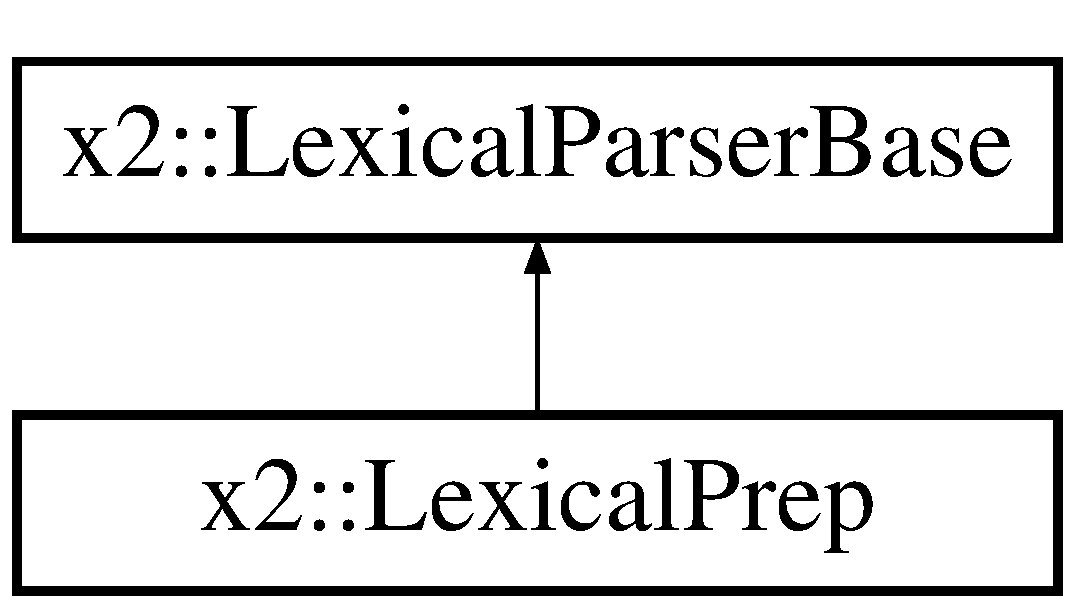
\includegraphics[height=2.000000cm]{classx2_1_1_lexical_parser_base}
\end{center}
\end{figure}
\subsection*{Public Member Functions}
\begin{DoxyCompactItemize}
\item 
\mbox{\Hypertarget{classx2_1_1_lexical_parser_base_a3db73300fe1d9a3ebb9778c0b11aa345}\label{classx2_1_1_lexical_parser_base_a3db73300fe1d9a3ebb9778c0b11aa345}} 
virtual void {\bfseries parse} (const char $\ast$buffer, size\+\_\+t len, size\+\_\+t \&index)=0
\item 
\mbox{\Hypertarget{classx2_1_1_lexical_parser_base_a5cb3232295603aca19cf732db66c3709}\label{classx2_1_1_lexical_parser_base_a5cb3232295603aca19cf732db66c3709}} 
virtual void {\bfseries error} (const char $\ast$buffer, size\+\_\+t len, size\+\_\+t \&index, int \&state)=0
\item 
\mbox{\Hypertarget{classx2_1_1_lexical_parser_base_a7070565fd2865aeba4145f396722833d}\label{classx2_1_1_lexical_parser_base_a7070565fd2865aeba4145f396722833d}} 
virtual int {\bfseries get\+Next\+State} (int cur\+State, char ch)=0
\end{DoxyCompactItemize}


The documentation for this class was generated from the following file\+:\begin{DoxyCompactItemize}
\item 
D\+:/\+Pool/eclipse-\/workspace/compiler-\/debug/include/Lexical\+Parser.\+h\end{DoxyCompactItemize}

\hypertarget{classx2_1_1_lexical_prep}{}\section{x2\+:\+:Lexical\+Prep Class Reference}
\label{classx2_1_1_lexical_prep}\index{x2\+::\+Lexical\+Prep@{x2\+::\+Lexical\+Prep}}
Inheritance diagram for x2\+:\+:Lexical\+Prep\+:\begin{figure}[H]
\begin{center}
\leavevmode
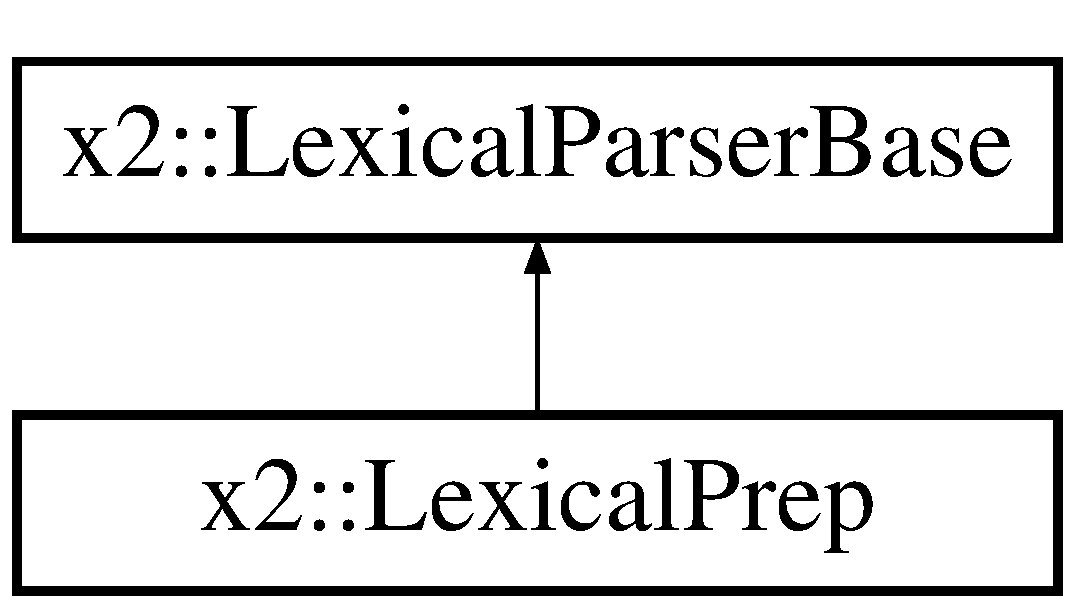
\includegraphics[height=2.000000cm]{classx2_1_1_lexical_prep}
\end{center}
\end{figure}
\subsection*{Public Types}
\begin{DoxyCompactItemize}
\item 
\mbox{\Hypertarget{classx2_1_1_lexical_prep_a824c45c7a34058d731b60324815a8384}\label{classx2_1_1_lexical_prep_a824c45c7a34058d731b60324815a8384}} 
enum \{ \newline
{\bfseries S\+T\+A\+T\+E\+\_\+\+L\+A\+ST} =-\/1, 
{\bfseries S\+T\+A\+T\+E\+\_\+\+E\+R\+R\+OR} =-\/2, 
{\bfseries S\+T\+A\+T\+E\+\_\+\+S\+T\+A\+RT} =0, 
{\bfseries S\+T\+A\+T\+E\+\_\+\+T\+R\+A\+N\+S\+F\+ER}, 
\newline
{\bfseries S\+T\+A\+T\+E\+\_\+\+I\+D\+\_\+\+S\+T\+A\+RT}, 
{\bfseries S\+T\+A\+T\+E\+\_\+\+I\+D\+\_\+\+E\+ND}, 
{\bfseries S\+T\+A\+T\+E\+\_\+\+N\+U\+M\+B\+ER}, 
{\bfseries S\+T\+A\+T\+E\+\_\+\+D\+I\+R\+E\+C\+T\+I\+V\+E\+\_\+\+S\+T\+A\+RT}, 
\newline
{\bfseries S\+T\+A\+T\+E\+\_\+\+D\+I\+R\+E\+C\+T\+I\+V\+E\+\_\+\+E\+ND}
 \}
\item 
\mbox{\Hypertarget{classx2_1_1_lexical_prep_a2d842e29a3f190c8e8aab0158e2f2d8d}\label{classx2_1_1_lexical_prep_a2d842e29a3f190c8e8aab0158e2f2d8d}} 
enum \{ \newline
{\bfseries S\+E\+T\+\_\+\+S\+T\+A\+RT} =-\/1000, 
{\bfseries S\+E\+T\+\_\+\+B\+IN}, 
{\bfseries S\+E\+T\+\_\+\+H\+EX}, 
{\bfseries S\+E\+T\+\_\+\+D\+EC}, 
\newline
{\bfseries S\+E\+T\+\_\+\+L\+O\+W\+ER}, 
{\bfseries S\+E\+T\+\_\+\+U\+P\+P\+ER}, 
{\bfseries S\+E\+T\+\_\+\+L\+E\+T\+T\+ER}, 
{\bfseries S\+E\+T\+\_\+\+W\+O\+R\+D\+\_\+\+S\+T\+A\+RT}, 
\newline
{\bfseries S\+E\+T\+\_\+\+W\+O\+R\+D\+\_\+\+E\+ND}, 
{\bfseries S\+E\+T\+\_\+\+I\+N\+L\+I\+N\+E\+\_\+\+S\+P\+A\+CE}, 
{\bfseries S\+E\+T\+\_\+\+S\+P\+A\+CE}, 
{\bfseries S\+E\+T\+\_\+\+N\+O\+N\+\_\+\+W\+O\+RD}
 \}
\item 
\mbox{\Hypertarget{classx2_1_1_lexical_prep_a85dac42b31f4e252c5bd41225ddc8192}\label{classx2_1_1_lexical_prep_a85dac42b31f4e252c5bd41225ddc8192}} 
typedef \hyperlink{classx2_1_1_lexical_prep}{Lexical\+Prep} {\bfseries This}
\item 
\mbox{\Hypertarget{classx2_1_1_lexical_prep_a5dfa1a4f6a396958da74affec6c1df67}\label{classx2_1_1_lexical_prep_a5dfa1a4f6a396958da74affec6c1df67}} 
typedef std\+::map$<$ int, std\+::map$<$ int, int $>$ $>$ {\bfseries Trans\+Map}
\end{DoxyCompactItemize}
\subsection*{Public Member Functions}
\begin{DoxyCompactItemize}
\item 
\mbox{\Hypertarget{classx2_1_1_lexical_prep_ad13cec8bb420d73eeee81a9ec179b1a1}\label{classx2_1_1_lexical_prep_ad13cec8bb420d73eeee81a9ec179b1a1}} 
{\bfseries Lexical\+Prep} (int i)
\item 
\mbox{\Hypertarget{classx2_1_1_lexical_prep_ab53c6c59c506b4622f9f9cb98c334c95}\label{classx2_1_1_lexical_prep_ab53c6c59c506b4622f9f9cb98c334c95}} 
void {\bfseries parse} (const char $\ast$buffer, size\+\_\+t len, size\+\_\+t \&index)
\item 
\mbox{\Hypertarget{classx2_1_1_lexical_prep_aaa47b259983af53f1b7731c3577f24c2}\label{classx2_1_1_lexical_prep_aaa47b259983af53f1b7731c3577f24c2}} 
int {\bfseries get\+Next\+State} (int cur\+State, char ch)
\item 
\mbox{\Hypertarget{classx2_1_1_lexical_prep_abde0d268131038bd92c45b0e1d686fa8}\label{classx2_1_1_lexical_prep_abde0d268131038bd92c45b0e1d686fa8}} 
void {\bfseries error} (const char $\ast$buffer, size\+\_\+t len, size\+\_\+t \&index, int \&state)
\end{DoxyCompactItemize}
\subsection*{Protected Attributes}
\begin{DoxyCompactItemize}
\item 
\mbox{\Hypertarget{classx2_1_1_lexical_prep_a0e6e7b8dc9e35fbc65db5c95359a156e}\label{classx2_1_1_lexical_prep_a0e6e7b8dc9e35fbc65db5c95359a156e}} 
Trans\+Map {\bfseries trans\+Map}
\end{DoxyCompactItemize}


The documentation for this class was generated from the following file\+:\begin{DoxyCompactItemize}
\item 
D\+:/\+Pool/eclipse-\/workspace/compiler-\/debug/include/Lexical\+Parser.\+h\end{DoxyCompactItemize}

\hypertarget{classx2_1_1_lexical_to_grammar_stream}{}\section{x2\+:\+:Lexical\+To\+Grammar\+Stream Class Reference}
\label{classx2_1_1_lexical_to_grammar_stream}\index{x2\+::\+Lexical\+To\+Grammar\+Stream@{x2\+::\+Lexical\+To\+Grammar\+Stream}}


{\ttfamily \#include $<$Lexical\+Parser.\+h$>$}

Inheritance diagram for x2\+:\+:Lexical\+To\+Grammar\+Stream\+:\begin{figure}[H]
\begin{center}
\leavevmode
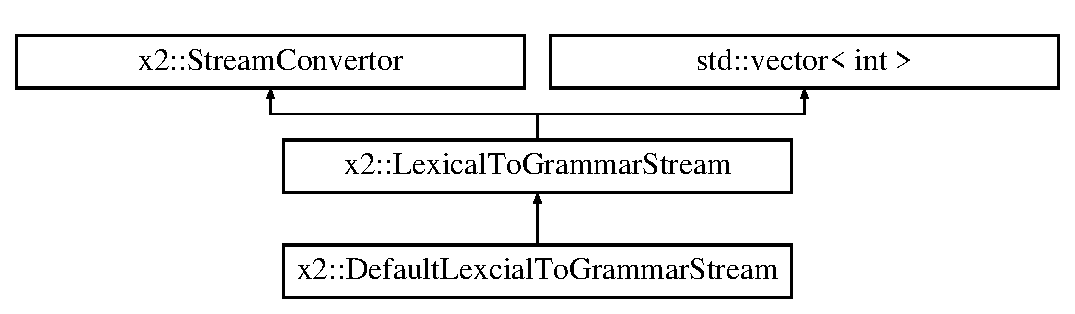
\includegraphics[height=3.000000cm]{classx2_1_1_lexical_to_grammar_stream}
\end{center}
\end{figure}
\subsection*{Public Types}
\begin{DoxyCompactItemize}
\item 
\mbox{\Hypertarget{classx2_1_1_lexical_to_grammar_stream_a06ae6e58b3913bb1b693759831e0ba0d}\label{classx2_1_1_lexical_to_grammar_stream_a06ae6e58b3913bb1b693759831e0ba0d}} 
typedef \hyperlink{classx2_1_1_lexical_to_grammar_stream}{Lexical\+To\+Grammar\+Stream} {\bfseries This}
\item 
\mbox{\Hypertarget{classx2_1_1_lexical_to_grammar_stream_a76f44ca6e2d0341489f6a2ab0680d5c4}\label{classx2_1_1_lexical_to_grammar_stream_a76f44ca6e2d0341489f6a2ab0680d5c4}} 
typedef \hyperlink{classx2_1_1_stream_convertor}{Stream\+Convertor} {\bfseries Father}
\item 
\mbox{\Hypertarget{classx2_1_1_lexical_to_grammar_stream_a9acac6d22837802e8559d64ac827c799}\label{classx2_1_1_lexical_to_grammar_stream_a9acac6d22837802e8559d64ac827c799}} 
using {\bfseries Size\+Type} = std\+::vector$<$ int $>$\+::size\+\_\+type
\end{DoxyCompactItemize}
\subsection*{Public Member Functions}
\begin{DoxyCompactItemize}
\item 
\mbox{\Hypertarget{classx2_1_1_lexical_to_grammar_stream_a393596cd9ceaabd4a4fdf0a7fcea4a2c}\label{classx2_1_1_lexical_to_grammar_stream_a393596cd9ceaabd4a4fdf0a7fcea4a2c}} 
{\bfseries Lexical\+To\+Grammar\+Stream} (std\+::initializer\+\_\+list$<$ int $>$ list)
\item 
\mbox{\Hypertarget{classx2_1_1_lexical_to_grammar_stream_aae745125e58536eb4e56ec821723031a}\label{classx2_1_1_lexical_to_grammar_stream_aae745125e58536eb4e56ec821723031a}} 
{\bfseries Lexical\+To\+Grammar\+Stream} (std\+::vector$<$ int $>$ \&\&list)
\item 
\mbox{\Hypertarget{classx2_1_1_lexical_to_grammar_stream_a334aecb6568d8f30bfac37860b99833d}\label{classx2_1_1_lexical_to_grammar_stream_a334aecb6568d8f30bfac37860b99833d}} 
{\bfseries Lexical\+To\+Grammar\+Stream} (const vector$<$ int $>$ \&list)
\item 
\mbox{\Hypertarget{classx2_1_1_lexical_to_grammar_stream_ad4c04605d8dbb125211f79ecc8b9322d}\label{classx2_1_1_lexical_to_grammar_stream_ad4c04605d8dbb125211f79ecc8b9322d}} 
{\bfseries Lexical\+To\+Grammar\+Stream} (const \hyperlink{classx2_1_1_lexical_to_grammar_stream}{Lexical\+To\+Grammar\+Stream} \&stream)=default
\item 
\mbox{\Hypertarget{classx2_1_1_lexical_to_grammar_stream_affeee9707cacd9923627104ab667a8c6}\label{classx2_1_1_lexical_to_grammar_stream_affeee9707cacd9923627104ab667a8c6}} 
{\bfseries Lexical\+To\+Grammar\+Stream} (\hyperlink{classx2_1_1_lexical_to_grammar_stream}{Lexical\+To\+Grammar\+Stream} \&\&stream)=default
\item 
\mbox{\Hypertarget{classx2_1_1_lexical_to_grammar_stream_ac0aadf8b4d8a98218accbd6983f40c85}\label{classx2_1_1_lexical_to_grammar_stream_ac0aadf8b4d8a98218accbd6983f40c85}} 
virtual void {\bfseries move} (int i)
\item 
\mbox{\Hypertarget{classx2_1_1_lexical_to_grammar_stream_a120b0b329f7dbc1dce5c4fd5614be764}\label{classx2_1_1_lexical_to_grammar_stream_a120b0b329f7dbc1dce5c4fd5614be764}} 
virtual void {\bfseries go\+Head} ()
\item 
\mbox{\Hypertarget{classx2_1_1_lexical_to_grammar_stream_a418c04a6f99d13068bcfafae19a5fcf5}\label{classx2_1_1_lexical_to_grammar_stream_a418c04a6f99d13068bcfafae19a5fcf5}} 
virtual void {\bfseries go\+End} ()
\item 
virtual \hyperlink{classx2_1_1_stream_convertor}{Stream\+Convertor} \& \hyperlink{classx2_1_1_lexical_to_grammar_stream_a7b3d4b7bfc44a17905bae8dc8dcf7a40}{operator$>$$>$} (int \&i)
\item 
virtual int \hyperlink{classx2_1_1_lexical_to_grammar_stream_a67a0e2b6ed998fd1dea1c9829be4461f}{peek} () const
\item 
virtual int \hyperlink{classx2_1_1_lexical_to_grammar_stream_a8ae8e1b6ada26785c70db1255daca798}{get} ()
\item 
virtual bool \hyperlink{classx2_1_1_lexical_to_grammar_stream_a813ec919763970d4150f35cba4da1db1}{eof} () const
\end{DoxyCompactItemize}
\subsection*{Protected Attributes}
\begin{DoxyCompactItemize}
\item 
\mbox{\Hypertarget{classx2_1_1_lexical_to_grammar_stream_a7691e61d5ed3c843e1011f7733fab0c7}\label{classx2_1_1_lexical_to_grammar_stream_a7691e61d5ed3c843e1011f7733fab0c7}} 
Size\+Type {\bfseries cur\+Index}
\end{DoxyCompactItemize}


\subsection{Detailed Description}
at every get,peek or $>$$>$ operation,it\textquotesingle{}s the user\textquotesingle{}s obligation to check if the stream reaches its eof. 

\subsection{Member Function Documentation}
\mbox{\Hypertarget{classx2_1_1_lexical_to_grammar_stream_a813ec919763970d4150f35cba4da1db1}\label{classx2_1_1_lexical_to_grammar_stream_a813ec919763970d4150f35cba4da1db1}} 
\index{x2\+::\+Lexical\+To\+Grammar\+Stream@{x2\+::\+Lexical\+To\+Grammar\+Stream}!eof@{eof}}
\index{eof@{eof}!x2\+::\+Lexical\+To\+Grammar\+Stream@{x2\+::\+Lexical\+To\+Grammar\+Stream}}
\subsubsection{\texorpdfstring{eof()}{eof()}}
{\footnotesize\ttfamily bool x2\+::\+Lexical\+To\+Grammar\+Stream\+::eof (\begin{DoxyParamCaption}{ }\end{DoxyParamCaption}) const\hspace{0.3cm}{\ttfamily [inline]}, {\ttfamily [virtual]}}

judge if the stream is coming its ending 

Implements \hyperlink{classx2_1_1_stream_convertor_a64febc08c310555497ca497df583b940}{x2\+::\+Stream\+Convertor}.

\mbox{\Hypertarget{classx2_1_1_lexical_to_grammar_stream_a8ae8e1b6ada26785c70db1255daca798}\label{classx2_1_1_lexical_to_grammar_stream_a8ae8e1b6ada26785c70db1255daca798}} 
\index{x2\+::\+Lexical\+To\+Grammar\+Stream@{x2\+::\+Lexical\+To\+Grammar\+Stream}!get@{get}}
\index{get@{get}!x2\+::\+Lexical\+To\+Grammar\+Stream@{x2\+::\+Lexical\+To\+Grammar\+Stream}}
\subsubsection{\texorpdfstring{get()}{get()}}
{\footnotesize\ttfamily int x2\+::\+Lexical\+To\+Grammar\+Stream\+::get (\begin{DoxyParamCaption}{ }\end{DoxyParamCaption})\hspace{0.3cm}{\ttfamily [inline]}, {\ttfamily [virtual]}}

same with operator$>$$>$ 

Implements \hyperlink{classx2_1_1_stream_convertor_a1025f8d8b1b1e430a6476d74e2506b10}{x2\+::\+Stream\+Convertor}.

\mbox{\Hypertarget{classx2_1_1_lexical_to_grammar_stream_a7b3d4b7bfc44a17905bae8dc8dcf7a40}\label{classx2_1_1_lexical_to_grammar_stream_a7b3d4b7bfc44a17905bae8dc8dcf7a40}} 
\index{x2\+::\+Lexical\+To\+Grammar\+Stream@{x2\+::\+Lexical\+To\+Grammar\+Stream}!operator$>$$>$@{operator$>$$>$}}
\index{operator$>$$>$@{operator$>$$>$}!x2\+::\+Lexical\+To\+Grammar\+Stream@{x2\+::\+Lexical\+To\+Grammar\+Stream}}
\subsubsection{\texorpdfstring{operator$>$$>$()}{operator>>()}}
{\footnotesize\ttfamily \hyperlink{classx2_1_1_stream_convertor}{Stream\+Convertor} \& x2\+::\+Lexical\+To\+Grammar\+Stream\+::operator$>$$>$ (\begin{DoxyParamCaption}\item[{int \&}]{i }\end{DoxyParamCaption})\hspace{0.3cm}{\ttfamily [inline]}, {\ttfamily [virtual]}}

The 3 following getting operations do not check the index,so it may cause index out of range exception 

Implements \hyperlink{classx2_1_1_stream_convertor_a5b387cc560794db5ac2f0c35dd4023d1}{x2\+::\+Stream\+Convertor}.

\mbox{\Hypertarget{classx2_1_1_lexical_to_grammar_stream_a67a0e2b6ed998fd1dea1c9829be4461f}\label{classx2_1_1_lexical_to_grammar_stream_a67a0e2b6ed998fd1dea1c9829be4461f}} 
\index{x2\+::\+Lexical\+To\+Grammar\+Stream@{x2\+::\+Lexical\+To\+Grammar\+Stream}!peek@{peek}}
\index{peek@{peek}!x2\+::\+Lexical\+To\+Grammar\+Stream@{x2\+::\+Lexical\+To\+Grammar\+Stream}}
\subsubsection{\texorpdfstring{peek()}{peek()}}
{\footnotesize\ttfamily int x2\+::\+Lexical\+To\+Grammar\+Stream\+::peek (\begin{DoxyParamCaption}{ }\end{DoxyParamCaption}) const\hspace{0.3cm}{\ttfamily [inline]}, {\ttfamily [virtual]}}

get an input, but do not move the stream 

Implements \hyperlink{classx2_1_1_stream_convertor_a9bc76cb1b81f1b11c9967f37f01bf2be}{x2\+::\+Stream\+Convertor}.



The documentation for this class was generated from the following file\+:\begin{DoxyCompactItemize}
\item 
D\+:/\+Pool/eclipse-\/workspace/compiler-\/debug/include/Lexical\+Parser.\+h\end{DoxyCompactItemize}

\hypertarget{classx2_1_1_l_r1_gramma}{}\section{x2\+:\+:L\+R1\+Gramma Class Reference}
\label{classx2_1_1_l_r1_gramma}\index{x2\+::\+L\+R1\+Gramma@{x2\+::\+L\+R1\+Gramma}}


{\ttfamily \#include $<$Gramma\+Utils.\+h$>$}

Inheritance diagram for x2\+:\+:L\+R1\+Gramma\+:\begin{figure}[H]
\begin{center}
\leavevmode
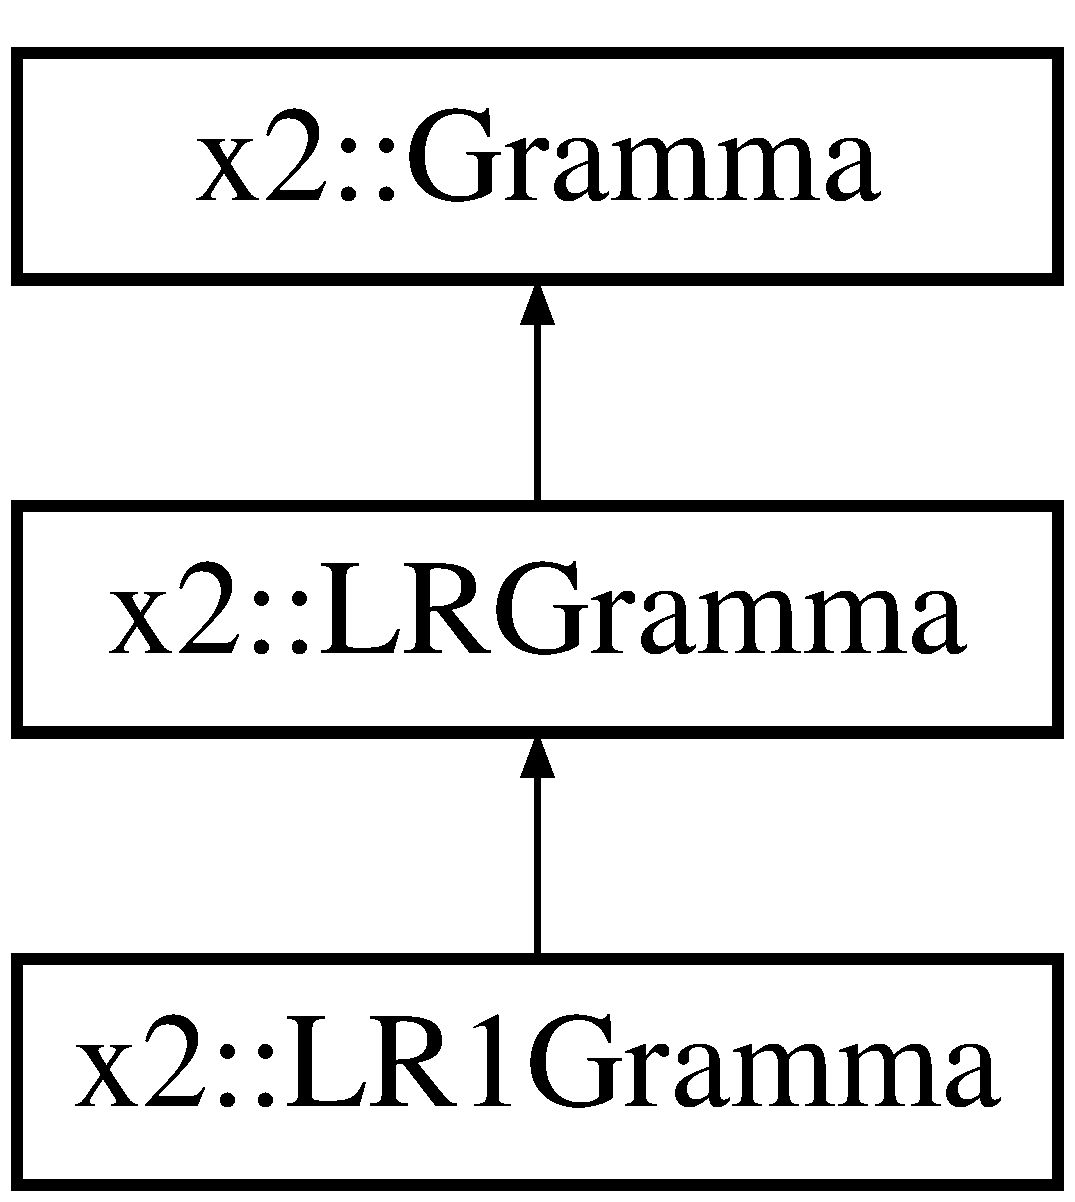
\includegraphics[height=3.000000cm]{classx2_1_1_l_r1_gramma}
\end{center}
\end{figure}
\subsection*{Public Types}
\begin{DoxyCompactItemize}
\item 
\mbox{\Hypertarget{classx2_1_1_l_r1_gramma_a8414ee258d00cf8d590cd983a0fe7465}\label{classx2_1_1_l_r1_gramma_a8414ee258d00cf8d590cd983a0fe7465}} 
enum {\bfseries A\+C\+T\+I\+O\+N\+\_\+\+T\+Y\+PE} \{ {\bfseries A\+C\+T\+I\+O\+N\+\_\+\+S\+H\+I\+F\+T\+\_\+\+IN}, 
{\bfseries A\+C\+T\+I\+O\+N\+\_\+\+R\+E\+D\+U\+CE}, 
{\bfseries A\+C\+T\+I\+O\+N\+\_\+\+A\+C\+C\+E\+PT}, 
{\bfseries A\+C\+T\+I\+O\+N\+\_\+\+E\+R\+R\+OR}
 \}
\item 
\mbox{\Hypertarget{classx2_1_1_l_r1_gramma_a030a0572b868d847a663fee42e00011b}\label{classx2_1_1_l_r1_gramma_a030a0572b868d847a663fee42e00011b}} 
typedef \hyperlink{classx2_1_1_l_r1_gramma}{L\+R1\+Gramma} {\bfseries This}
\item 
\mbox{\Hypertarget{classx2_1_1_l_r1_gramma_a218431439b832892e36f7eaae2beb4c2}\label{classx2_1_1_l_r1_gramma_a218431439b832892e36f7eaae2beb4c2}} 
typedef \hyperlink{classx2_1_1_l_r_gramma}{L\+R\+Gramma} {\bfseries Father}
\item 
\mbox{\Hypertarget{classx2_1_1_l_r1_gramma_af651f585181b1fceff704dba8dc5ebcc}\label{classx2_1_1_l_r1_gramma_af651f585181b1fceff704dba8dc5ebcc}} 
typedef std\+::tuple$<$ int, int, int, int $>$ {\bfseries Item\+Type}
\item 
\mbox{\Hypertarget{classx2_1_1_l_r1_gramma_acf6e4450e836fec8cd5c87d110e26ea9}\label{classx2_1_1_l_r1_gramma_acf6e4450e836fec8cd5c87d110e26ea9}} 
typedef std\+::set$<$ Item\+Type $>$ {\bfseries Closure\+Type}
\item 
\mbox{\Hypertarget{classx2_1_1_l_r1_gramma_a0bfe3e4cb0ef43da0823e520be4d461e}\label{classx2_1_1_l_r1_gramma_a0bfe3e4cb0ef43da0823e520be4d461e}} 
typedef std\+::vector$<$ Closure\+Type $>$ {\bfseries Closures\+Vector}
\item 
\mbox{\Hypertarget{classx2_1_1_l_r1_gramma_a96d8b7263ffce6eaf1ba10d3daa7afdc}\label{classx2_1_1_l_r1_gramma_a96d8b7263ffce6eaf1ba10d3daa7afdc}} 
typedef std\+::map$<$ std\+::pair$<$ int, int $>$, int $>$ {\bfseries Goto\+Info\+Type}
\item 
\mbox{\Hypertarget{classx2_1_1_l_r1_gramma_a77b658cf079a64b28967cfa7f977bd08}\label{classx2_1_1_l_r1_gramma_a77b658cf079a64b28967cfa7f977bd08}} 
typedef std\+::tuple$<$ Closures\+Vector, std\+::set$<$ int $>$, Goto\+Info\+Type $>$ {\bfseries Info\+Type}
\end{DoxyCompactItemize}
\subsection*{Public Member Functions}
\begin{DoxyCompactItemize}
\item 
\mbox{\Hypertarget{classx2_1_1_l_r1_gramma_afbd87724adfa33474132478f303209f5}\label{classx2_1_1_l_r1_gramma_afbd87724adfa33474132478f303209f5}} 
A\+S\+\_\+\+M\+A\+C\+RO {\bfseries L\+R1\+Gramma} (const \hyperlink{classx2_1_1_l_r_gramma}{L\+R\+Gramma} \&lrg)
\item 
\mbox{\Hypertarget{classx2_1_1_l_r1_gramma_a29beef6aeb9b6519184e892d8a44e902}\label{classx2_1_1_l_r1_gramma_a29beef6aeb9b6519184e892d8a44e902}} 
A\+S\+\_\+\+M\+A\+C\+RO {\bfseries L\+R1\+Gramma} (\hyperlink{classx2_1_1_l_r_gramma}{L\+R\+Gramma} \&\&lrg)
\item 
\mbox{\Hypertarget{classx2_1_1_l_r1_gramma_ace12408a94981c7d15256e1a7acf37a0}\label{classx2_1_1_l_r1_gramma_ace12408a94981c7d15256e1a7acf37a0}} 
A\+S\+\_\+\+M\+A\+C\+RO {\bfseries L\+R1\+Gramma} (const std\+::initializer\+\_\+list$<$ std\+::pair$<$ int, std\+::string $>$ $>$ \&list, const std\+::initializer\+\_\+list$<$ std\+::pair$<$ int, \hyperlink{classx2_1_1_gramma_sentence}{Gramma\+Sentence} $>$ $>$ \&prodlist, int oristart, int oriend, const std\+::string \&strstart)
\item 
\mbox{\Hypertarget{classx2_1_1_l_r1_gramma_aa3812220d4cc3f0b9a1d5a67245c015e}\label{classx2_1_1_l_r1_gramma_aa3812220d4cc3f0b9a1d5a67245c015e}} 
{\bfseries L\+R1\+Gramma} (const \hyperlink{classx2_1_1_gramma}{Gramma} \&g, const std\+::string \&ori\+Start, const std\+::string \&ori\+End, const std\+::string \&ext\+Start)
\item 
\mbox{\Hypertarget{classx2_1_1_l_r1_gramma_a887c2408e69595d589138e99ce9154a6}\label{classx2_1_1_l_r1_gramma_a887c2408e69595d589138e99ce9154a6}} 
{\bfseries L\+R1\+Gramma} (\hyperlink{classx2_1_1_gramma}{Gramma} \&\&g, const std\+::string \&ori\+Start, const std\+::string \&ori\+End, const std\+::string \&ext\+Start)
\item 
\mbox{\Hypertarget{classx2_1_1_l_r1_gramma_aff9f83c0779f9d638488bb3a112d8dd2}\label{classx2_1_1_l_r1_gramma_aff9f83c0779f9d638488bb3a112d8dd2}} 
Closure\+Type {\bfseries get\+Closure} (const Item\+Type \&i)
\item 
\mbox{\Hypertarget{classx2_1_1_l_r1_gramma_ac764feebd3d5afcc0afd828afefbbe83}\label{classx2_1_1_l_r1_gramma_ac764feebd3d5afcc0afd828afefbbe83}} 
Closure\+Type {\bfseries get\+Closure} (const Item\+Type \&i, const Gramma\+::\+Sets\+Type \&firstset)
\item 
\mbox{\Hypertarget{classx2_1_1_l_r1_gramma_a1ee889288311a6db3305ee6d1fed5f05}\label{classx2_1_1_l_r1_gramma_a1ee889288311a6db3305ee6d1fed5f05}} 
void {\bfseries get\+Closure} (const Item\+Type \&i, Closure\+Type \&C, const Gramma\+::\+Sets\+Type \&firstset)
\item 
\mbox{\Hypertarget{classx2_1_1_l_r1_gramma_a961277ef6df314f2edf297210cebe61a}\label{classx2_1_1_l_r1_gramma_a961277ef6df314f2edf297210cebe61a}} 
Closure\+Type {\bfseries get\+Closure} (const Closure\+Type \&C, const Gramma\+::\+Sets\+Type \&firstset)
\item 
\mbox{\Hypertarget{classx2_1_1_l_r1_gramma_a359e41207d7a512fb5316d0114764400}\label{classx2_1_1_l_r1_gramma_a359e41207d7a512fb5316d0114764400}} 
Closure\+Type {\bfseries get\+Goto} (const Closure\+Type \&clo, int x, const Gramma\+::\+Sets\+Type \&firstset)
\item 
\mbox{\Hypertarget{classx2_1_1_l_r1_gramma_af9718deaf1e08d45b7fba8f7a8dac40e}\label{classx2_1_1_l_r1_gramma_af9718deaf1e08d45b7fba8f7a8dac40e}} 
Info\+Type {\bfseries get\+All\+Closures} ()
\item 
\hyperlink{classx2_1_1_gramma_a03901eb5b196689b901fbf23e5bb9f0e}{L\+R\+Corrupt\+Table\+Type} \hyperlink{classx2_1_1_l_r1_gramma_ad8e8029481aa8f4ed2990c458ae8e162}{construct\+Analyze\+Table} (const Info\+Type \&info)
\item 
\mbox{\Hypertarget{classx2_1_1_l_r1_gramma_a8a29870586642ef45f2a564ae8a6e3b1}\label{classx2_1_1_l_r1_gramma_a8a29870586642ef45f2a564ae8a6e3b1}} 
A\+S\+\_\+\+M\+A\+C\+RO int {\bfseries get\+First\+Symbol\+After\+Dot} (const Item\+Type \&i)
\item 
int \hyperlink{classx2_1_1_l_r1_gramma_abefaef2936a830dd6e4ae26edeaff0d5}{get\+Nth\+Symbole\+After\+Dot} (const Item\+Type \&i, unsigned int j)
\item 
A\+S\+\_\+\+M\+A\+C\+RO std\+::string \hyperlink{classx2_1_1_l_r1_gramma_a80e8b8e656a431117f1b26a39164281f}{to\+String} () const
\item 
\mbox{\Hypertarget{classx2_1_1_l_r1_gramma_a7fe9aee546e52353260b791500c4c901}\label{classx2_1_1_l_r1_gramma_a7fe9aee546e52353260b791500c4c901}} 
std\+::string {\bfseries to\+String} (const Item\+Type \&i) const
\item 
\mbox{\Hypertarget{classx2_1_1_l_r1_gramma_a7bd9d52d8dca89b8f80d2fbc510781e1}\label{classx2_1_1_l_r1_gramma_a7bd9d52d8dca89b8f80d2fbc510781e1}} 
std\+::string {\bfseries to\+String} (const Closure\+Type \&closure) const
\item 
\mbox{\Hypertarget{classx2_1_1_l_r1_gramma_a5377a952f9b644679486562c1541ff47}\label{classx2_1_1_l_r1_gramma_a5377a952f9b644679486562c1541ff47}} 
std\+::string {\bfseries to\+String} (const Info\+Type \&info) const
\item 
\mbox{\Hypertarget{classx2_1_1_l_r1_gramma_afbbf6899bed1091fbc33df05a5e5993f}\label{classx2_1_1_l_r1_gramma_afbbf6899bed1091fbc33df05a5e5993f}} 
std\+::string {\bfseries to\+String} (const \hyperlink{classx2_1_1_gramma_a33681053b045219ea58cc68c3faa4975}{L\+R\+Analyze\+Table\+Type} \&table\+Info) const
\item 
\mbox{\Hypertarget{classx2_1_1_l_r1_gramma_a483fccba9ab1e14e7132d79b2cb80ab0}\label{classx2_1_1_l_r1_gramma_a483fccba9ab1e14e7132d79b2cb80ab0}} 
std\+::string {\bfseries to\+String} (const \hyperlink{classx2_1_1_gramma_a03901eb5b196689b901fbf23e5bb9f0e}{L\+R\+Corrupt\+Table\+Type} \&table\+Info) const
\end{DoxyCompactItemize}
\subsection*{Static Public Member Functions}
\begin{DoxyCompactItemize}
\item 
static A\+S\+\_\+\+M\+A\+C\+RO bool \hyperlink{classx2_1_1_l_r1_gramma_a47cbb98b8eceeae4600067e29f4d67b6}{do\+Insert} (Closure\+Type \&C, const Item\+Type \&i)
\end{DoxyCompactItemize}
\subsection*{Static Public Attributes}
\begin{DoxyCompactItemize}
\item 
static std\+::unordered\+\_\+map$<$ int, std\+::string $>$ {\bfseries A\+C\+T\+I\+O\+N\+\_\+\+I\+N\+F\+O\+\_\+\+S\+T\+R\+I\+NG}
\end{DoxyCompactItemize}
\subsection*{Additional Inherited Members}


\subsection{Detailed Description}
L\+R1 \hyperlink{classx2_1_1_gramma}{Gramma} each item is a 4-\/tuple\+: L\+R0\+Item plus a terminator 

\subsection{Member Function Documentation}
\mbox{\Hypertarget{classx2_1_1_l_r1_gramma_ad8e8029481aa8f4ed2990c458ae8e162}\label{classx2_1_1_l_r1_gramma_ad8e8029481aa8f4ed2990c458ae8e162}} 
\index{x2\+::\+L\+R1\+Gramma@{x2\+::\+L\+R1\+Gramma}!construct\+Analyze\+Table@{construct\+Analyze\+Table}}
\index{construct\+Analyze\+Table@{construct\+Analyze\+Table}!x2\+::\+L\+R1\+Gramma@{x2\+::\+L\+R1\+Gramma}}
\subsubsection{\texorpdfstring{construct\+Analyze\+Table()}{constructAnalyzeTable()}}
{\footnotesize\ttfamily \hyperlink{classx2_1_1_gramma_a03901eb5b196689b901fbf23e5bb9f0e}{L\+R1\+Gramma\+::\+L\+R\+Corrupt\+Table\+Type} x2\+::\+L\+R1\+Gramma\+::construct\+Analyze\+Table (\begin{DoxyParamCaption}\item[{const Info\+Type \&}]{info }\end{DoxyParamCaption})}

constructing algorithm\+: 构造项目集规范族和\+G\+O\+TO 对项目集规范族中的每一项\+Ii 对\+Ii中的每一项 \mbox{[}A-\/$>$C.\+DE,b\mbox{]},如果\+D不是变量 如果\+D是终结符号,则\+A\+C\+T\+I\+ON\mbox{[}i,D\mbox{]}=移入\+G\+O\+T\+O(i,\+D)的值 如果\+D是空(表明一定不是S\textquotesingle{}-\/$>$S.),将\+A\+C\+T\+I\+ON\mbox{[}i,a\mbox{]}设置为规约\+A-\/$>$C.\+DE 如果\+D是结束符号,意味着b也是结束符号,设置\+A\+C\+T\+I\+ON\mbox{[}i,\$\mbox{]}=接受 //如果上面的循环出现重复,就意味着冲突,则这个文法不是\+LR(1)的 //还应当返回冲突信息 Corrupt\+Type,这是\+A\+C\+T\+I\+O\+N类型的扩展集,它可以在一个转移上支持多个状态

对于没有设置的项,默认为\+E\+R\+R\+OR 初始状态是\+I0 \mbox{\Hypertarget{classx2_1_1_l_r1_gramma_a47cbb98b8eceeae4600067e29f4d67b6}\label{classx2_1_1_l_r1_gramma_a47cbb98b8eceeae4600067e29f4d67b6}} 
\index{x2\+::\+L\+R1\+Gramma@{x2\+::\+L\+R1\+Gramma}!do\+Insert@{do\+Insert}}
\index{do\+Insert@{do\+Insert}!x2\+::\+L\+R1\+Gramma@{x2\+::\+L\+R1\+Gramma}}
\subsubsection{\texorpdfstring{do\+Insert()}{doInsert()}}
{\footnotesize\ttfamily A\+S\+\_\+\+M\+A\+C\+RO bool x2\+::\+L\+R1\+Gramma\+::do\+Insert (\begin{DoxyParamCaption}\item[{Closure\+Type \&}]{C,  }\item[{const Item\+Type \&}]{i }\end{DoxyParamCaption})\hspace{0.3cm}{\ttfamily [static]}}

insert i in C, if really updated,return true;

return false (means no update) \mbox{\Hypertarget{classx2_1_1_l_r1_gramma_abefaef2936a830dd6e4ae26edeaff0d5}\label{classx2_1_1_l_r1_gramma_abefaef2936a830dd6e4ae26edeaff0d5}} 
\index{x2\+::\+L\+R1\+Gramma@{x2\+::\+L\+R1\+Gramma}!get\+Nth\+Symbole\+After\+Dot@{get\+Nth\+Symbole\+After\+Dot}}
\index{get\+Nth\+Symbole\+After\+Dot@{get\+Nth\+Symbole\+After\+Dot}!x2\+::\+L\+R1\+Gramma@{x2\+::\+L\+R1\+Gramma}}
\subsubsection{\texorpdfstring{get\+Nth\+Symbole\+After\+Dot()}{getNthSymboleAfterDot()}}
{\footnotesize\ttfamily int x2\+::\+L\+R1\+Gramma\+::get\+Nth\+Symbole\+After\+Dot (\begin{DoxyParamCaption}\item[{const Item\+Type \&}]{i,  }\item[{unsigned int}]{j }\end{DoxyParamCaption})}

j=0 return E\+M\+P\+TY j=1 return first j=2 return second \mbox{\Hypertarget{classx2_1_1_l_r1_gramma_a80e8b8e656a431117f1b26a39164281f}\label{classx2_1_1_l_r1_gramma_a80e8b8e656a431117f1b26a39164281f}} 
\index{x2\+::\+L\+R1\+Gramma@{x2\+::\+L\+R1\+Gramma}!to\+String@{to\+String}}
\index{to\+String@{to\+String}!x2\+::\+L\+R1\+Gramma@{x2\+::\+L\+R1\+Gramma}}
\subsubsection{\texorpdfstring{to\+String()}{toString()}}
{\footnotesize\ttfamily std\+::string x2\+::\+L\+R1\+Gramma\+::to\+String (\begin{DoxyParamCaption}{ }\end{DoxyParamCaption}) const}

依据优先级和结合性来消除冲突.

看优先级,相同优先级看结合性 具体规则\+: 保留最高优先级的产生式 在同优先级的产生式组中,保留归约式中的一个 

\subsection{Member Data Documentation}
\mbox{\Hypertarget{classx2_1_1_l_r1_gramma_a3f17e2d9cd35551d2dc3314a76dc60d7}\label{classx2_1_1_l_r1_gramma_a3f17e2d9cd35551d2dc3314a76dc60d7}} 
\index{x2\+::\+L\+R1\+Gramma@{x2\+::\+L\+R1\+Gramma}!A\+C\+T\+I\+O\+N\+\_\+\+I\+N\+F\+O\+\_\+\+S\+T\+R\+I\+NG@{A\+C\+T\+I\+O\+N\+\_\+\+I\+N\+F\+O\+\_\+\+S\+T\+R\+I\+NG}}
\index{A\+C\+T\+I\+O\+N\+\_\+\+I\+N\+F\+O\+\_\+\+S\+T\+R\+I\+NG@{A\+C\+T\+I\+O\+N\+\_\+\+I\+N\+F\+O\+\_\+\+S\+T\+R\+I\+NG}!x2\+::\+L\+R1\+Gramma@{x2\+::\+L\+R1\+Gramma}}
\subsubsection{\texorpdfstring{A\+C\+T\+I\+O\+N\+\_\+\+I\+N\+F\+O\+\_\+\+S\+T\+R\+I\+NG}{ACTION\_INFO\_STRING}}
{\footnotesize\ttfamily std\+::unordered\+\_\+map$<$ int, std\+::string $>$ x2\+::\+L\+R1\+Gramma\+::\+A\+C\+T\+I\+O\+N\+\_\+\+I\+N\+F\+O\+\_\+\+S\+T\+R\+I\+NG\hspace{0.3cm}{\ttfamily [static]}}

{\bfseries Initial value\+:}
\begin{DoxyCode}
=\{
          \{ACTION\_ACCEPT,\textcolor{stringliteral}{"ACCEPT"}\},
          \{ACTION\_SHIFT\_IN,\textcolor{stringliteral}{"SHIFT"}\},
          \{ACTION\_ERROR,\textcolor{stringliteral}{"ERROR"}\},
          \{ACTION\_REDUCE,\textcolor{stringliteral}{"REDUCE"}\},
  \}
\end{DoxyCode}


The documentation for this class was generated from the following files\+:\begin{DoxyCompactItemize}
\item 
D\+:/\+Pool/eclipse-\/workspace/compiler-\/debug/include/Gramma\+Utils.\+h\item 
D\+:/\+Pool/eclipse-\/workspace/compiler-\/debug/src/Gramma\+Utils.\+cpp\end{DoxyCompactItemize}

\hypertarget{classx2_1_1_l_r_gramma}{}\section{x2\+:\+:L\+R\+Gramma Class Reference}
\label{classx2_1_1_l_r_gramma}\index{x2\+::\+L\+R\+Gramma@{x2\+::\+L\+R\+Gramma}}


{\ttfamily \#include $<$Gramma\+Utils.\+h$>$}

Inheritance diagram for x2\+:\+:L\+R\+Gramma\+:\begin{figure}[H]
\begin{center}
\leavevmode
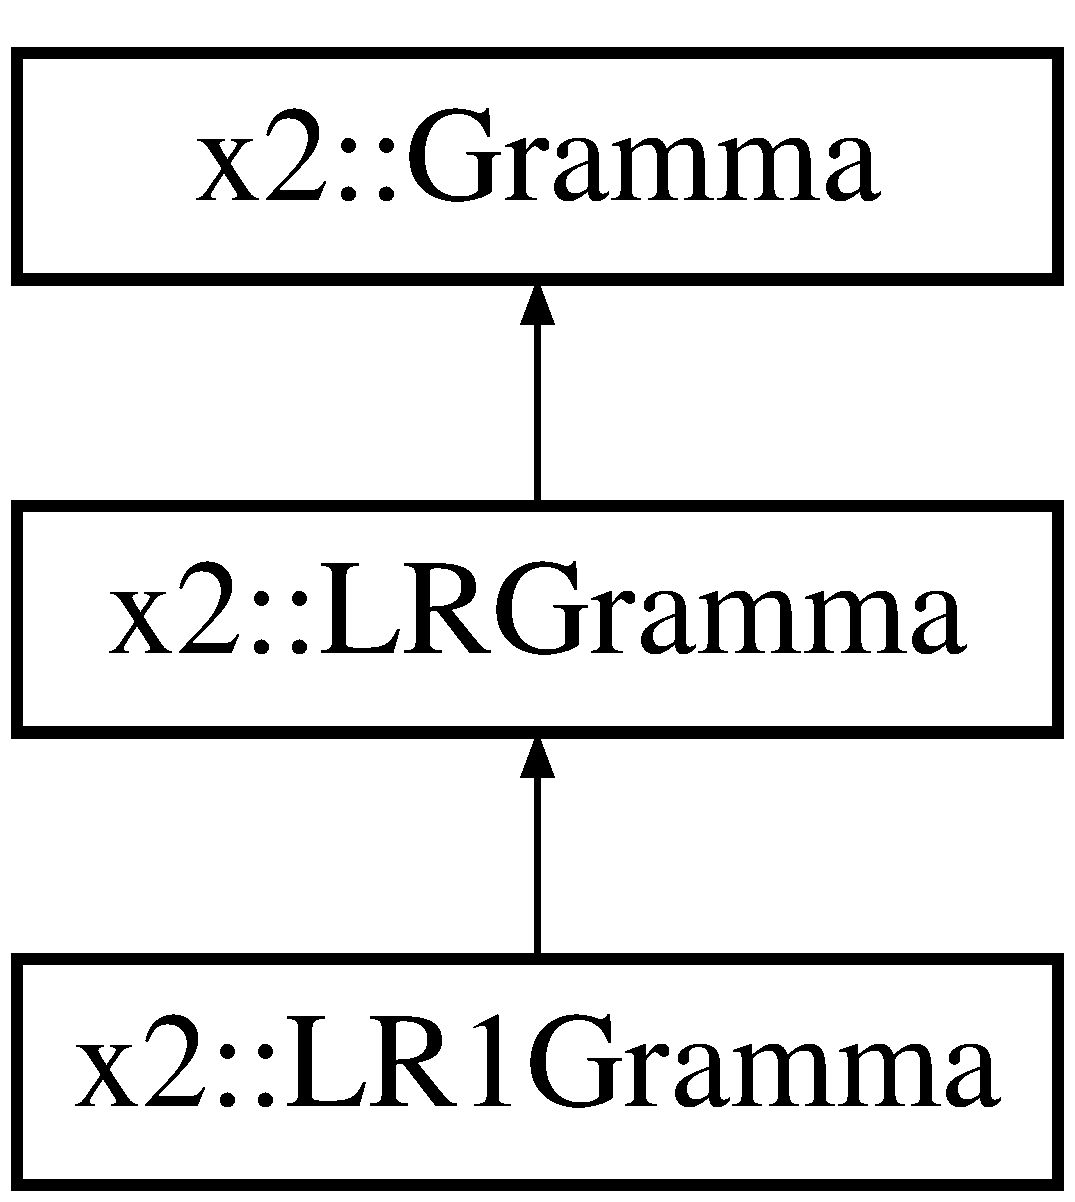
\includegraphics[height=3.000000cm]{classx2_1_1_l_r_gramma}
\end{center}
\end{figure}
\subsection*{Public Types}
\begin{DoxyCompactItemize}
\item 
\mbox{\Hypertarget{classx2_1_1_l_r_gramma_a71192f7005e3f0369414c888a73be237}\label{classx2_1_1_l_r_gramma_a71192f7005e3f0369414c888a73be237}} 
typedef \hyperlink{classx2_1_1_l_r_gramma}{L\+R\+Gramma} {\bfseries This}
\item 
\mbox{\Hypertarget{classx2_1_1_l_r_gramma_a4841e95ceda2580dcb28924cde7eccf3}\label{classx2_1_1_l_r_gramma_a4841e95ceda2580dcb28924cde7eccf3}} 
typedef \hyperlink{classx2_1_1_gramma}{Gramma} {\bfseries Father}
\item 
\mbox{\Hypertarget{classx2_1_1_l_r_gramma_ad6ec096bc4670fccd2e4778314d2e0cb}\label{classx2_1_1_l_r_gramma_ad6ec096bc4670fccd2e4778314d2e0cb}} 
typedef std\+::tuple$<$ int, int, int $>$ {\bfseries Item\+Type}
\item 
\mbox{\Hypertarget{classx2_1_1_l_r_gramma_a8df1989466f03aecabd14ec34ba6433b}\label{classx2_1_1_l_r_gramma_a8df1989466f03aecabd14ec34ba6433b}} 
typedef std\+::set$<$ Item\+Type $>$ {\bfseries Closure\+Type}
\item 
\mbox{\Hypertarget{classx2_1_1_l_r_gramma_a5d21d307296ccff26e15c9e0b1c13dfb}\label{classx2_1_1_l_r_gramma_a5d21d307296ccff26e15c9e0b1c13dfb}} 
typedef std\+::vector$<$ Closure\+Type $>$ {\bfseries Closures\+Vector}
\item 
\mbox{\Hypertarget{classx2_1_1_l_r_gramma_a5622c230cf16f9def37f4b61c7db4c20}\label{classx2_1_1_l_r_gramma_a5622c230cf16f9def37f4b61c7db4c20}} 
typedef std\+::tuple$<$ Closures\+Vector, std\+::set$<$ int $>$, std\+::map$<$ std\+::pair$<$ int, int $>$, int $>$ $>$ {\bfseries Info\+Type}
\end{DoxyCompactItemize}
\subsection*{Public Member Functions}
\begin{DoxyCompactItemize}
\item 
\hyperlink{classx2_1_1_l_r_gramma_aaf38ee87d4dd3be25b48356f204ab17f}{L\+R\+Gramma} ()=default
\item 
\mbox{\Hypertarget{classx2_1_1_l_r_gramma_ad8567e4bafe68acd70fb93b98da3afc9}\label{classx2_1_1_l_r_gramma_ad8567e4bafe68acd70fb93b98da3afc9}} 
{\bfseries L\+R\+Gramma} (const \hyperlink{classx2_1_1_l_r_gramma}{L\+R\+Gramma} \&lrg)=default
\item 
\mbox{\Hypertarget{classx2_1_1_l_r_gramma_a15273d95cdfeca70fbbaf22afd78213a}\label{classx2_1_1_l_r_gramma_a15273d95cdfeca70fbbaf22afd78213a}} 
{\bfseries L\+R\+Gramma} (\hyperlink{classx2_1_1_l_r_gramma}{L\+R\+Gramma} \&\&lrg)=default
\item 
\mbox{\Hypertarget{classx2_1_1_l_r_gramma_a06de326709a3656338a6dc0f18ba8c1f}\label{classx2_1_1_l_r_gramma_a06de326709a3656338a6dc0f18ba8c1f}} 
{\bfseries L\+R\+Gramma} (const \hyperlink{classx2_1_1_gramma}{Gramma} \&g, int oristart, int oriend, const std\+::string \&strstart)
\item 
\mbox{\Hypertarget{classx2_1_1_l_r_gramma_af5c52d1d6ced5980fbe4859bdcad130c}\label{classx2_1_1_l_r_gramma_af5c52d1d6ced5980fbe4859bdcad130c}} 
{\bfseries L\+R\+Gramma} (\hyperlink{classx2_1_1_gramma}{Gramma} \&\&g, int oristart, int oriend, const std\+::string \&strstart)
\item 
\mbox{\Hypertarget{classx2_1_1_l_r_gramma_a89bb2afe42f616a2ee9ba2efa41c103b}\label{classx2_1_1_l_r_gramma_a89bb2afe42f616a2ee9ba2efa41c103b}} 
{\bfseries L\+R\+Gramma} (const std\+::initializer\+\_\+list$<$ std\+::pair$<$ int, std\+::string $>$ $>$ \&list, const std\+::initializer\+\_\+list$<$ std\+::pair$<$ int, \hyperlink{classx2_1_1_gramma_sentence}{Gramma\+Sentence} $>$ $>$ \&prodlist, int oristart, int oriend, const std\+::string \&strstart)
\item 
\mbox{\Hypertarget{classx2_1_1_l_r_gramma_a2732ee4cc51030f039cf5f90b5475a51}\label{classx2_1_1_l_r_gramma_a2732ee4cc51030f039cf5f90b5475a51}} 
{\bfseries L\+R\+Gramma} (const \hyperlink{classx2_1_1_gramma_symbols}{Gramma\+Symbols} \&gs, const Productions\+Type \&prods, int oristart, int oriend, const std\+::string \&strstart)
\item 
\mbox{\Hypertarget{classx2_1_1_l_r_gramma_ae9b5a9130670906995f24b328f04e825}\label{classx2_1_1_l_r_gramma_ae9b5a9130670906995f24b328f04e825}} 
{\bfseries L\+R\+Gramma} (const \hyperlink{classx2_1_1_gramma_symbols}{Gramma\+Symbols} \&gs, Productions\+Type \&\&prods, int oristart, int oriend, const std\+::string \&strstart)
\item 
\mbox{\Hypertarget{classx2_1_1_l_r_gramma_aaa21674847491a3145be5c3ba32c094d}\label{classx2_1_1_l_r_gramma_aaa21674847491a3145be5c3ba32c094d}} 
{\bfseries L\+R\+Gramma} (\hyperlink{classx2_1_1_gramma_symbols}{Gramma\+Symbols} \&\&gs, const Productions\+Type \&prods, int oristart, int oriend, const std\+::string \&strstart)
\item 
\mbox{\Hypertarget{classx2_1_1_l_r_gramma_aee0d20fc4dea94380d6912ddd6b526c7}\label{classx2_1_1_l_r_gramma_aee0d20fc4dea94380d6912ddd6b526c7}} 
{\bfseries L\+R\+Gramma} (\hyperlink{classx2_1_1_gramma_symbols}{Gramma\+Symbols} \&\&gs, Productions\+Type \&\&prods, int oristart, int oriend, const std\+::string \&strstart)
\item 
\mbox{\Hypertarget{classx2_1_1_l_r_gramma_a1c9cea6688bcf7ec1dce11cdcceb4189}\label{classx2_1_1_l_r_gramma_a1c9cea6688bcf7ec1dce11cdcceb4189}} 
{\bfseries L\+R\+Gramma} (const \hyperlink{classx2_1_1_gramma}{Gramma} \&g, const std\+::string \&ori\+Start, const std\+::string \&ori\+End, const std\+::string \&ext\+Start)
\item 
\mbox{\Hypertarget{classx2_1_1_l_r_gramma_a89d445f6a3d58250f486d5261afca6fd}\label{classx2_1_1_l_r_gramma_a89d445f6a3d58250f486d5261afca6fd}} 
{\bfseries L\+R\+Gramma} (\hyperlink{classx2_1_1_gramma}{Gramma} \&\&g, const std\+::string \&ori\+Start, const std\+::string \&ori\+End, const std\+::string \&ext\+Start)
\item 
Info\+Type \hyperlink{classx2_1_1_l_r_gramma_a03deaa81155f09b014629b32769b8228}{get\+All\+Closures} ()
\item 
\hyperlink{classx2_1_1_gramma_a03901eb5b196689b901fbf23e5bb9f0e}{L\+R\+Corrupt\+Table\+Type} \hyperlink{classx2_1_1_l_r_gramma_a93fdb0ff53f9960980ff955b318e1883}{construct\+Analyze\+Table\+L\+R0} (const Info\+Type \&info)
\item 
\mbox{\Hypertarget{classx2_1_1_l_r_gramma_a0d56a6e69eccb330110304642ca0aca2}\label{classx2_1_1_l_r_gramma_a0d56a6e69eccb330110304642ca0aca2}} 
\hyperlink{classx2_1_1_gramma_a03901eb5b196689b901fbf23e5bb9f0e}{L\+R\+Corrupt\+Table\+Type} {\bfseries construct\+Analyze\+Table\+S\+LR} (const Info\+Type \&info)
\item 
int \hyperlink{classx2_1_1_l_r_gramma_a6f9db2e24c2f5ccdbeb7f2a5c3e6f46e}{get\+Closure\+In\+Vector} (const Item\+Type \&i, Closures\+Vector \&itemsets, std\+::map$<$ Item\+Type, int $>$ \&C0)
\item 
\mbox{\Hypertarget{classx2_1_1_l_r_gramma_aa2b002dcbb20cbc063f45e0c91bcaf92}\label{classx2_1_1_l_r_gramma_aa2b002dcbb20cbc063f45e0c91bcaf92}} 
Closure\+Type {\bfseries get\+Closure} (const Item\+Type \&i)
\item 
\mbox{\Hypertarget{classx2_1_1_l_r_gramma_a68fcd9ffac09218b72d5188e37bd3330}\label{classx2_1_1_l_r_gramma_a68fcd9ffac09218b72d5188e37bd3330}} 
void {\bfseries get\+Closure} (const Item\+Type \&i, Closure\+Type \&C)
\item 
\mbox{\Hypertarget{classx2_1_1_l_r_gramma_ac8ddf976b25cfbc6088653a341a95e14}\label{classx2_1_1_l_r_gramma_ac8ddf976b25cfbc6088653a341a95e14}} 
Closure\+Type {\bfseries get\+Closure} (const Closure\+Type \&C)
\item 
Closure\+Type \hyperlink{classx2_1_1_l_r_gramma_a933cdf18c4a8515dbeef0cea0bdaf04e}{get\+Goto\+In\+Vector} (int iclo, int x, Closures\+Vector \&itemsets, std\+::map$<$ Item\+Type, int $>$ \&C0)
\item 
\mbox{\Hypertarget{classx2_1_1_l_r_gramma_aed7c1b2c750a4267d2482849efa80a0c}\label{classx2_1_1_l_r_gramma_aed7c1b2c750a4267d2482849efa80a0c}} 
Closure\+Type {\bfseries get\+Goto} (const Closure\+Type \&items, int x)
\item 
\mbox{\Hypertarget{classx2_1_1_l_r_gramma_af93dc3f5f2754571065efcb5db90c61d}\label{classx2_1_1_l_r_gramma_af93dc3f5f2754571065efcb5db90c61d}} 
A\+S\+\_\+\+M\+A\+C\+RO int {\bfseries get\+First\+Symbol\+After\+Dot} (const Item\+Type \&i)
\item 
\mbox{\Hypertarget{classx2_1_1_l_r_gramma_a264d5976acad1bcbbca757ff2732cda2}\label{classx2_1_1_l_r_gramma_a264d5976acad1bcbbca757ff2732cda2}} 
int {\bfseries get\+Nth\+Symbole\+After\+Dot} (const Item\+Type \&i, unsigned int j)
\item 
\mbox{\Hypertarget{classx2_1_1_l_r_gramma_a3e5af1beed3487756cb31d7e1fe8f680}\label{classx2_1_1_l_r_gramma_a3e5af1beed3487756cb31d7e1fe8f680}} 
A\+S\+\_\+\+M\+A\+C\+RO int {\bfseries get\+Ext\+Start} () const
\item 
\mbox{\Hypertarget{classx2_1_1_l_r_gramma_aac75b15832f2ccba608d5caefe3f66ba}\label{classx2_1_1_l_r_gramma_aac75b15832f2ccba608d5caefe3f66ba}} 
A\+S\+\_\+\+M\+A\+C\+RO int {\bfseries get\+End} () const
\item 
\mbox{\Hypertarget{classx2_1_1_l_r_gramma_a687589eac850af2bcdb012b740531a2e}\label{classx2_1_1_l_r_gramma_a687589eac850af2bcdb012b740531a2e}} 
A\+S\+\_\+\+M\+A\+C\+RO std\+::string {\bfseries to\+String} () const
\item 
\mbox{\Hypertarget{classx2_1_1_l_r_gramma_a0de96313ac9b29148dcf146fcae9af45}\label{classx2_1_1_l_r_gramma_a0de96313ac9b29148dcf146fcae9af45}} 
std\+::string {\bfseries to\+String} (const Item\+Type \&item) const
\item 
\mbox{\Hypertarget{classx2_1_1_l_r_gramma_a91003d63b709ba51c5d1759ec89d61f4}\label{classx2_1_1_l_r_gramma_a91003d63b709ba51c5d1759ec89d61f4}} 
std\+::string {\bfseries to\+String} (const Closure\+Type \&closure) const
\item 
\mbox{\Hypertarget{classx2_1_1_l_r_gramma_a1a15ca465ccc7d3b77a5e8780f519fa1}\label{classx2_1_1_l_r_gramma_a1a15ca465ccc7d3b77a5e8780f519fa1}} 
std\+::string {\bfseries to\+String} (const std\+::tuple$<$ Closures\+Vector, std\+::set$<$ int $>$, std\+::map$<$ std\+::pair$<$ int, int $>$, int $>$$>$ \&tups) const
\item 
\mbox{\Hypertarget{classx2_1_1_l_r_gramma_acd4d44e2d8b4a0d06599431bae7bad86}\label{classx2_1_1_l_r_gramma_acd4d44e2d8b4a0d06599431bae7bad86}} 
std\+::string {\bfseries to\+String\+Set} (int i) const
\item 
\mbox{\Hypertarget{classx2_1_1_l_r_gramma_a66728cb47718f3041fb797ef2992a55e}\label{classx2_1_1_l_r_gramma_a66728cb47718f3041fb797ef2992a55e}} 
A\+S\+\_\+\+M\+A\+C\+RO void {\bfseries set\+Dot\+String} (const std\+::string \&s)
\end{DoxyCompactItemize}
\subsection*{Public Attributes}
\begin{DoxyCompactItemize}
\item 
\mbox{\Hypertarget{classx2_1_1_l_r_gramma_adac4892cff5dc2a78380612d7bb31597}\label{classx2_1_1_l_r_gramma_adac4892cff5dc2a78380612d7bb31597}} 
int {\bfseries sstart}
\item 
\mbox{\Hypertarget{classx2_1_1_l_r_gramma_a2e2226f01f334f7aec6f2a13c4e614f3}\label{classx2_1_1_l_r_gramma_a2e2226f01f334f7aec6f2a13c4e614f3}} 
int {\bfseries send}
\item 
\mbox{\Hypertarget{classx2_1_1_l_r_gramma_a9a36e830070363ce6b50d36bef3efd88}\label{classx2_1_1_l_r_gramma_a9a36e830070363ce6b50d36bef3efd88}} 
std\+::string {\bfseries dot\+String}
\end{DoxyCompactItemize}
\subsection*{Static Public Attributes}
\begin{DoxyCompactItemize}
\item 
\mbox{\Hypertarget{classx2_1_1_l_r_gramma_a2349263521150b34859af413c5dbbc2c}\label{classx2_1_1_l_r_gramma_a2349263521150b34859af413c5dbbc2c}} 
static const std\+::string {\bfseries D\+O\+T\+\_\+\+S\+T\+R\+I\+NG} =\char`\"{}.\char`\"{}
\end{DoxyCompactItemize}
\subsection*{Additional Inherited Members}


\subsection{Detailed Description}
General Model\+: i,j --$>$ which production? k --$>$ position of the dot

//\+L\+R1 s --$>$ symbol of looking ahead

known types \+: L\+R(0) Items, L\+R(1) Items, S\+L\+R(1) items L\+A\+L\+R(1) items 从广泛的意义上来说(就行为层面),每个项目类型的 Closure,Goto,Analyse Table,求法是有所不同的 统一的接口就是 接受某个通用文法作为参数,计算某个项目集的\+Closure

除此之外,to\+String方法也是不同的 但是它们的分析表类型都是一样的 不必将 项目集真正地存入语法之中,因为一个语法的项目集要么不求,要么整体求出,通常是一个计算的过程 不必缓存 \hyperlink{classx2_1_1_l_r_gramma}{L\+R\+Gramma} 

\subsection{Constructor \& Destructor Documentation}
\mbox{\Hypertarget{classx2_1_1_l_r_gramma_aaf38ee87d4dd3be25b48356f204ab17f}\label{classx2_1_1_l_r_gramma_aaf38ee87d4dd3be25b48356f204ab17f}} 
\index{x2\+::\+L\+R\+Gramma@{x2\+::\+L\+R\+Gramma}!L\+R\+Gramma@{L\+R\+Gramma}}
\index{L\+R\+Gramma@{L\+R\+Gramma}!x2\+::\+L\+R\+Gramma@{x2\+::\+L\+R\+Gramma}}
\subsubsection{\texorpdfstring{L\+R\+Gramma()}{LRGramma()}}
{\footnotesize\ttfamily x2\+::\+L\+R\+Gramma\+::\+L\+R\+Gramma (\begin{DoxyParamCaption}{ }\end{DoxyParamCaption})\hspace{0.3cm}{\ttfamily [default]}}

这里的\+Closure\+Type和教材上类型有所不同,教材上的类型是 std\+::map$<$std\+::set$<$\+Item\+Type$>$,std\+::set$<$\+Item\+Type$>$$>$ Closure\+Type 这里为了方便,先定义单个项的闭包 如果是多个项 Closure(I1,I2,...,In) = Closure(\+I1) u Closure(\+I2) u ... u Closure(\+In) 

\subsection{Member Function Documentation}
\mbox{\Hypertarget{classx2_1_1_l_r_gramma_a93fdb0ff53f9960980ff955b318e1883}\label{classx2_1_1_l_r_gramma_a93fdb0ff53f9960980ff955b318e1883}} 
\index{x2\+::\+L\+R\+Gramma@{x2\+::\+L\+R\+Gramma}!construct\+Analyze\+Table\+L\+R0@{construct\+Analyze\+Table\+L\+R0}}
\index{construct\+Analyze\+Table\+L\+R0@{construct\+Analyze\+Table\+L\+R0}!x2\+::\+L\+R\+Gramma@{x2\+::\+L\+R\+Gramma}}
\subsubsection{\texorpdfstring{construct\+Analyze\+Table\+L\+R0()}{constructAnalyzeTableLR0()}}
{\footnotesize\ttfamily \hyperlink{classx2_1_1_gramma_a03901eb5b196689b901fbf23e5bb9f0e}{L\+R\+Corrupt\+Table\+Type} x2\+::\+L\+R\+Gramma\+::construct\+Analyze\+Table\+L\+R0 (\begin{DoxyParamCaption}\item[{const Info\+Type \&}]{info }\end{DoxyParamCaption})}

added 2017-\/04-\/22 12\+:32\+:52 \mbox{\Hypertarget{classx2_1_1_l_r_gramma_a03deaa81155f09b014629b32769b8228}\label{classx2_1_1_l_r_gramma_a03deaa81155f09b014629b32769b8228}} 
\index{x2\+::\+L\+R\+Gramma@{x2\+::\+L\+R\+Gramma}!get\+All\+Closures@{get\+All\+Closures}}
\index{get\+All\+Closures@{get\+All\+Closures}!x2\+::\+L\+R\+Gramma@{x2\+::\+L\+R\+Gramma}}
\subsubsection{\texorpdfstring{get\+All\+Closures()}{getAllClosures()}}
{\footnotesize\ttfamily L\+R\+Gramma\+::\+Info\+Type x2\+::\+L\+R\+Gramma\+::get\+All\+Closures (\begin{DoxyParamCaption}{ }\end{DoxyParamCaption})}

return a tuple tuple\mbox{[}0\mbox{]} \+: contains closures that indexes in tuple\mbox{[}1\mbox{]} \& tuple\mbox{[}2\mbox{]} point to tuple\mbox{[}1\mbox{]} \+: a set of integers, those integers denote the concanical item sets of the gramma tuple\mbox{[}2\mbox{]} \+: the goto map. the key type is pair$<$int,int$>$, the first int denotes a closure in tuple\mbox{[}0\mbox{]},the second is a possible gramma symbol.

call to\+String(tup) to dump those information. \mbox{\Hypertarget{classx2_1_1_l_r_gramma_a6f9db2e24c2f5ccdbeb7f2a5c3e6f46e}\label{classx2_1_1_l_r_gramma_a6f9db2e24c2f5ccdbeb7f2a5c3e6f46e}} 
\index{x2\+::\+L\+R\+Gramma@{x2\+::\+L\+R\+Gramma}!get\+Closure\+In\+Vector@{get\+Closure\+In\+Vector}}
\index{get\+Closure\+In\+Vector@{get\+Closure\+In\+Vector}!x2\+::\+L\+R\+Gramma@{x2\+::\+L\+R\+Gramma}}
\subsubsection{\texorpdfstring{get\+Closure\+In\+Vector()}{getClosureInVector()}}
{\footnotesize\ttfamily int x2\+::\+L\+R\+Gramma\+::get\+Closure\+In\+Vector (\begin{DoxyParamCaption}\item[{const Item\+Type \&}]{i,  }\item[{Closures\+Vector \&}]{itemsets,  }\item[{std\+::map$<$ Item\+Type, int $>$ \&}]{C0 }\end{DoxyParamCaption})}

H\+I\+G\+H-\/\+W\+AY get\+Closure == shut down//deprecated 可能产生新的闭包

if not set, then set at the end,get \mbox{\Hypertarget{classx2_1_1_l_r_gramma_a933cdf18c4a8515dbeef0cea0bdaf04e}\label{classx2_1_1_l_r_gramma_a933cdf18c4a8515dbeef0cea0bdaf04e}} 
\index{x2\+::\+L\+R\+Gramma@{x2\+::\+L\+R\+Gramma}!get\+Goto\+In\+Vector@{get\+Goto\+In\+Vector}}
\index{get\+Goto\+In\+Vector@{get\+Goto\+In\+Vector}!x2\+::\+L\+R\+Gramma@{x2\+::\+L\+R\+Gramma}}
\subsubsection{\texorpdfstring{get\+Goto\+In\+Vector()}{getGotoInVector()}}
{\footnotesize\ttfamily L\+R\+Gramma\+::\+Closure\+Type x2\+::\+L\+R\+Gramma\+::get\+Goto\+In\+Vector (\begin{DoxyParamCaption}\item[{int}]{iclo,  }\item[{int}]{x,  }\item[{Closures\+Vector \&}]{itemsets,  }\item[{std\+::map$<$ Item\+Type, int $>$ \&}]{C0 }\end{DoxyParamCaption})}

H\+I\+G\+H-\/\+W\+AY get\+Goto == shut down//deprecated 

The documentation for this class was generated from the following files\+:\begin{DoxyCompactItemize}
\item 
D\+:/\+Pool/eclipse-\/workspace/compiler-\/debug/include/Gramma\+Utils.\+h\item 
D\+:/\+Pool/eclipse-\/workspace/compiler-\/debug/src/Gramma\+Utils.\+cpp\end{DoxyCompactItemize}

\hypertarget{classx2_1_1_mutual_map}{}\section{x2\+:\+:Mutual\+Map$<$ T1, T2 $>$ Class Template Reference}
\label{classx2_1_1_mutual_map}\index{x2\+::\+Mutual\+Map$<$ T1, T2 $>$@{x2\+::\+Mutual\+Map$<$ T1, T2 $>$}}


{\ttfamily \#include $<$Mutual\+Map.\+h$>$}

\subsection*{Public Types}
\begin{DoxyCompactItemize}
\item 
\mbox{\Hypertarget{classx2_1_1_mutual_map_aab4506822de38fe4801e6fd26dcfc4a8}\label{classx2_1_1_mutual_map_aab4506822de38fe4801e6fd26dcfc4a8}} 
typedef \hyperlink{classx2_1_1_mutual_map}{Mutual\+Map}$<$ T1, T2 $>$ {\bfseries This}
\item 
\mbox{\Hypertarget{classx2_1_1_mutual_map_a5b2d1fecd17aa67effd5f530f3bfcb77}\label{classx2_1_1_mutual_map_a5b2d1fecd17aa67effd5f530f3bfcb77}} 
typedef T1 {\bfseries Type1}
\item 
\mbox{\Hypertarget{classx2_1_1_mutual_map_afa9a6a304444f00fc24e2a643731ec6e}\label{classx2_1_1_mutual_map_afa9a6a304444f00fc24e2a643731ec6e}} 
typedef T2 {\bfseries Type2}
\item 
\mbox{\Hypertarget{classx2_1_1_mutual_map_a2b67e110065e0e79fb558e662980d6ba}\label{classx2_1_1_mutual_map_a2b67e110065e0e79fb558e662980d6ba}} 
typedef std\+::map$<$ Type1, Type2 $>$ {\bfseries Map\+Type1}
\item 
\mbox{\Hypertarget{classx2_1_1_mutual_map_a3d131315a967f500f9273ee5b41e9e72}\label{classx2_1_1_mutual_map_a3d131315a967f500f9273ee5b41e9e72}} 
typedef std\+::map$<$ Type2, Type1 $>$ {\bfseries Map\+Type2}
\end{DoxyCompactItemize}
\subsection*{Public Member Functions}
\begin{DoxyCompactItemize}
\item 
\mbox{\Hypertarget{classx2_1_1_mutual_map_a0aec006dfe740b3aca9b8f5cd3ede3e0}\label{classx2_1_1_mutual_map_a0aec006dfe740b3aca9b8f5cd3ede3e0}} 
{\bfseries Mutual\+Map} (const T1 \&failed\+T1, const T2 \&failed\+T2)
\item 
\mbox{\Hypertarget{classx2_1_1_mutual_map_acb2a15b336a6c70edd3d4fe9a26ee546}\label{classx2_1_1_mutual_map_acb2a15b336a6c70edd3d4fe9a26ee546}} 
{\bfseries Mutual\+Map} (const T1 \&failed\+T1, const T2 \&failed\+T2, std\+::initializer\+\_\+list$<$ std\+::pair$<$ T1, T2 $>$$>$ list)
\item 
\mbox{\Hypertarget{classx2_1_1_mutual_map_a0f8373a36782451417531b32de7ede92}\label{classx2_1_1_mutual_map_a0f8373a36782451417531b32de7ede92}} 
{\bfseries Mutual\+Map} (\hyperlink{classx2_1_1_mutual_map}{Mutual\+Map}$<$ T1, T2 $>$ \&\&mm)=default
\item 
\mbox{\Hypertarget{classx2_1_1_mutual_map_ac22842edf0d0c2ff714ecf863162d614}\label{classx2_1_1_mutual_map_ac22842edf0d0c2ff714ecf863162d614}} 
{\bfseries Mutual\+Map} (const \hyperlink{classx2_1_1_mutual_map}{Mutual\+Map}$<$ T1, T2 $>$ \&mm)=default
\item 
const T1 \& \hyperlink{classx2_1_1_mutual_map_acff746e0227b363d23d7a854a9673d44}{get\+T2} (const T2 \&t2) const
\item 
\mbox{\Hypertarget{classx2_1_1_mutual_map_ad0e2ed1c35c156ac7f379c737ea2a98d}\label{classx2_1_1_mutual_map_ad0e2ed1c35c156ac7f379c737ea2a98d}} 
const T2 \& {\bfseries get\+T1} (const T1 \&t1) const
\item 
const T1 \& \hyperlink{classx2_1_1_mutual_map_aba13a2fb8bd6343efc7874da48c5156c}{get\+Add\+T2} (const T2 \&t2, const T1 \&t1)
\item 
\mbox{\Hypertarget{classx2_1_1_mutual_map_aebbfcc0501af0e6080f71d6ca4c468df}\label{classx2_1_1_mutual_map_aebbfcc0501af0e6080f71d6ca4c468df}} 
const T2 \& {\bfseries get\+Add\+T1} (const T1 \&t1, const T2 \&t2)
\item 
bool \hyperlink{classx2_1_1_mutual_map_ac9572b3e52982e24e77978ee7e3ab44b}{add\+T1} (const T1 \&t1, const T2 \&t2)
\item 
\mbox{\Hypertarget{classx2_1_1_mutual_map_a3aff757ccd0b3c5adf5d91dd9b792bfd}\label{classx2_1_1_mutual_map_a3aff757ccd0b3c5adf5d91dd9b792bfd}} 
bool {\bfseries add\+T1} (T1 \&\&t1, T2 \&\&t2)
\item 
\mbox{\Hypertarget{classx2_1_1_mutual_map_a46bd0595e1983a9d4239a9c005ad45dc}\label{classx2_1_1_mutual_map_a46bd0595e1983a9d4239a9c005ad45dc}} 
bool {\bfseries add\+T2} (const T2 \&t2, const T1 \&t1)
\item 
\mbox{\Hypertarget{classx2_1_1_mutual_map_a585053ba0d6293850ca4af5b4a259cec}\label{classx2_1_1_mutual_map_a585053ba0d6293850ca4af5b4a259cec}} 
bool {\bfseries add\+T2} (T2 \&\&t2, T1 \&\&t1)
\item 
\mbox{\Hypertarget{classx2_1_1_mutual_map_a095d9b2f5e11716764c78e64a93f691d}\label{classx2_1_1_mutual_map_a095d9b2f5e11716764c78e64a93f691d}} 
T2 {\bfseries remove\+T1} (const T1 \&t1)
\item 
\mbox{\Hypertarget{classx2_1_1_mutual_map_a31ae2da8838537afba8bec8e0c560090}\label{classx2_1_1_mutual_map_a31ae2da8838537afba8bec8e0c560090}} 
T1 {\bfseries remove\+T2} (const T2 \&t2)
\item 
bool \hyperlink{classx2_1_1_mutual_map_adcf6a37d18e6db2939cb205c73ca9b72}{add\+Replace\+T1} (const T1 \&t1, const T2 \&t2)
\item 
\mbox{\Hypertarget{classx2_1_1_mutual_map_ad0e9896b9abf29c9a6a81b69511387f1}\label{classx2_1_1_mutual_map_ad0e9896b9abf29c9a6a81b69511387f1}} 
bool {\bfseries add\+Replace\+T2} (const T2 \&t2, const T1 \&t1)
\item 
\mbox{\Hypertarget{classx2_1_1_mutual_map_a79a7822f40483ef63a78100ed1700e6a}\label{classx2_1_1_mutual_map_a79a7822f40483ef63a78100ed1700e6a}} 
std\+::string {\bfseries to\+String} () const
\end{DoxyCompactItemize}
\subsection*{Protected Attributes}
\begin{DoxyCompactItemize}
\item 
\mbox{\Hypertarget{classx2_1_1_mutual_map_a85e97b24c0cc1633aadc3739fa60569b}\label{classx2_1_1_mutual_map_a85e97b24c0cc1633aadc3739fa60569b}} 
Map\+Type1 {\bfseries m1}
\item 
\mbox{\Hypertarget{classx2_1_1_mutual_map_a5f8f5940664f7842ad7b4c898a34e0a8}\label{classx2_1_1_mutual_map_a5f8f5940664f7842ad7b4c898a34e0a8}} 
Map\+Type2 {\bfseries m2}
\item 
\mbox{\Hypertarget{classx2_1_1_mutual_map_a6c536ae71190e39f0c9ab7d75dd2f160}\label{classx2_1_1_mutual_map_a6c536ae71190e39f0c9ab7d75dd2f160}} 
Type1 {\bfseries failed\+T1}
\item 
\mbox{\Hypertarget{classx2_1_1_mutual_map_a24c70f6ed99841b01ce43fa4514151c6}\label{classx2_1_1_mutual_map_a24c70f6ed99841b01ce43fa4514151c6}} 
Type2 {\bfseries failed\+T2}
\end{DoxyCompactItemize}


\subsection{Detailed Description}
\subsubsection*{template$<$class T1, class T2$>$\newline
class x2\+::\+Mutual\+Map$<$ T1, T2 $>$}

任意时刻保证: 如果a,b 在m1中,则b,a必在m2中;如果a,b在m2中,则b,a必在m1中 如果a,b不在m1中,则b,a不在m2中;如果a,b不在m2中,则b,a不在m1中

2017-\/4-\/26 20\+:59\+:09 为了使其可以容纳相同的类型映射,将方法名修改.

方法名 \+: add\+T1 和 add\+T2 分别表示以谁作为键来查询,添加和删除; 其中作为键的一方不会被删除或者修改 

\subsection{Member Function Documentation}
\mbox{\Hypertarget{classx2_1_1_mutual_map_adcf6a37d18e6db2939cb205c73ca9b72}\label{classx2_1_1_mutual_map_adcf6a37d18e6db2939cb205c73ca9b72}} 
\index{x2\+::\+Mutual\+Map@{x2\+::\+Mutual\+Map}!add\+Replace\+T1@{add\+Replace\+T1}}
\index{add\+Replace\+T1@{add\+Replace\+T1}!x2\+::\+Mutual\+Map@{x2\+::\+Mutual\+Map}}
\subsubsection{\texorpdfstring{add\+Replace\+T1()}{addReplaceT1()}}
{\footnotesize\ttfamily template$<$class T1, class T2$>$ \\
bool \hyperlink{classx2_1_1_mutual_map}{x2\+::\+Mutual\+Map}$<$ T1, T2 $>$\+::add\+Replace\+T1 (\begin{DoxyParamCaption}\item[{const T1 \&}]{t1,  }\item[{const T2 \&}]{t2 }\end{DoxyParamCaption})\hspace{0.3cm}{\ttfamily [inline]}}

add, if t1 pair already exist,then t1 is kept,change $<$t1,\+\_\+$>$ to $<$t1,t2$>$ return if replaced \mbox{\Hypertarget{classx2_1_1_mutual_map_ac9572b3e52982e24e77978ee7e3ab44b}\label{classx2_1_1_mutual_map_ac9572b3e52982e24e77978ee7e3ab44b}} 
\index{x2\+::\+Mutual\+Map@{x2\+::\+Mutual\+Map}!add\+T1@{add\+T1}}
\index{add\+T1@{add\+T1}!x2\+::\+Mutual\+Map@{x2\+::\+Mutual\+Map}}
\subsubsection{\texorpdfstring{add\+T1()}{addT1()}}
{\footnotesize\ttfamily template$<$class T1, class T2$>$ \\
bool \hyperlink{classx2_1_1_mutual_map}{x2\+::\+Mutual\+Map}$<$ T1, T2 $>$\+::add\+T1 (\begin{DoxyParamCaption}\item[{const T1 \&}]{t1,  }\item[{const T2 \&}]{t2 }\end{DoxyParamCaption})\hspace{0.3cm}{\ttfamily [inline]}}

if any one is present,return failed,else return succeed \mbox{\Hypertarget{classx2_1_1_mutual_map_aba13a2fb8bd6343efc7874da48c5156c}\label{classx2_1_1_mutual_map_aba13a2fb8bd6343efc7874da48c5156c}} 
\index{x2\+::\+Mutual\+Map@{x2\+::\+Mutual\+Map}!get\+Add\+T2@{get\+Add\+T2}}
\index{get\+Add\+T2@{get\+Add\+T2}!x2\+::\+Mutual\+Map@{x2\+::\+Mutual\+Map}}
\subsubsection{\texorpdfstring{get\+Add\+T2()}{getAddT2()}}
{\footnotesize\ttfamily template$<$class T1, class T2$>$ \\
const T1 \& \hyperlink{classx2_1_1_mutual_map}{x2\+::\+Mutual\+Map}$<$ T1, T2 $>$\+::get\+Add\+T2 (\begin{DoxyParamCaption}\item[{const T2 \&}]{t2,  }\item[{const T1 \&}]{t1 }\end{DoxyParamCaption})\hspace{0.3cm}{\ttfamily [inline]}}

get,if non-\/exist, add it \mbox{\Hypertarget{classx2_1_1_mutual_map_acff746e0227b363d23d7a854a9673d44}\label{classx2_1_1_mutual_map_acff746e0227b363d23d7a854a9673d44}} 
\index{x2\+::\+Mutual\+Map@{x2\+::\+Mutual\+Map}!get\+T2@{get\+T2}}
\index{get\+T2@{get\+T2}!x2\+::\+Mutual\+Map@{x2\+::\+Mutual\+Map}}
\subsubsection{\texorpdfstring{get\+T2()}{getT2()}}
{\footnotesize\ttfamily template$<$class T1 , class T2$>$ \\
const T1 \& \hyperlink{classx2_1_1_mutual_map}{x2\+::\+Mutual\+Map}$<$ T1, T2 $>$\+::get\+T2 (\begin{DoxyParamCaption}\item[{const T2 \&}]{t2 }\end{DoxyParamCaption}) const\hspace{0.3cm}{\ttfamily [inline]}}

两者都作为键,不可能直接更改其中任何一方的值 如果没有查找到,还应当 有一个默认的返回值,即提供失败的值 

The documentation for this class was generated from the following file\+:\begin{DoxyCompactItemize}
\item 
D\+:/\+Pool/eclipse-\/workspace/compiler-\/debug/include/Mutual\+Map.\+h\end{DoxyCompactItemize}

\hypertarget{classx2_1_1_nondeterminastic_f_a}{}\section{x2\+:\+:Nondeterminastic\+FA$<$ T $>$ Class Template Reference}
\label{classx2_1_1_nondeterminastic_f_a}\index{x2\+::\+Nondeterminastic\+F\+A$<$ T $>$@{x2\+::\+Nondeterminastic\+F\+A$<$ T $>$}}
Inheritance diagram for x2\+:\+:Nondeterminastic\+FA$<$ T $>$\+:\begin{figure}[H]
\begin{center}
\leavevmode
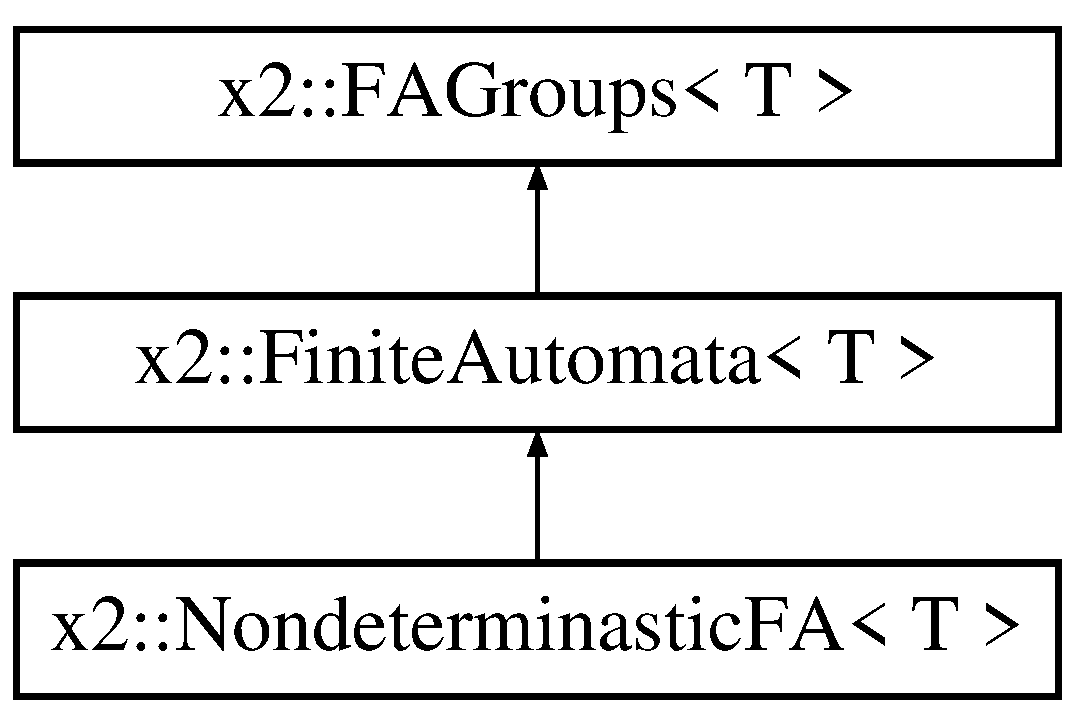
\includegraphics[height=3.000000cm]{classx2_1_1_nondeterminastic_f_a}
\end{center}
\end{figure}
\subsection*{Protected Attributes}
\begin{DoxyCompactItemize}
\item 
\mbox{\Hypertarget{classx2_1_1_nondeterminastic_f_a_a4e08a188366e00391a3dc3e9b20ee473}\label{classx2_1_1_nondeterminastic_f_a_a4e08a188366e00391a3dc3e9b20ee473}} 
std\+::map$<$ std\+::pair$<$ int, T $>$, std\+::set$<$ int $>$ $>$ {\bfseries transitions}
\end{DoxyCompactItemize}
\subsection*{Additional Inherited Members}


The documentation for this class was generated from the following file\+:\begin{DoxyCompactItemize}
\item 
D\+:/\+Pool/eclipse-\/workspace/compiler-\/debug/include/F\+A\+Utils.\+h\end{DoxyCompactItemize}

\hypertarget{classx2_1_1_output_stream_processor}{}\section{x2\+:\+:Output\+Stream\+Processor$<$ T $>$ Class Template Reference}
\label{classx2_1_1_output_stream_processor}\index{x2\+::\+Output\+Stream\+Processor$<$ T $>$@{x2\+::\+Output\+Stream\+Processor$<$ T $>$}}


{\ttfamily \#include $<$F\+A\+Utils.\+h$>$}

Inheritance diagram for x2\+:\+:Output\+Stream\+Processor$<$ T $>$\+:\begin{figure}[H]
\begin{center}
\leavevmode
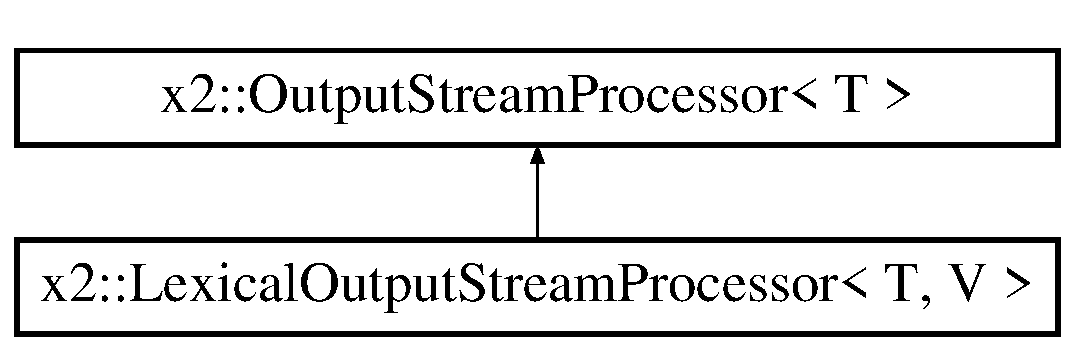
\includegraphics[height=2.000000cm]{classx2_1_1_output_stream_processor}
\end{center}
\end{figure}
\subsection*{Public Member Functions}
\begin{DoxyCompactItemize}
\item 
\mbox{\Hypertarget{classx2_1_1_output_stream_processor_af3cc85a55c0029e301aa2c9bcd80dcb8}\label{classx2_1_1_output_stream_processor_af3cc85a55c0029e301aa2c9bcd80dcb8}} 
virtual void {\bfseries process} (int cur\+State, const T \&in)=0
\end{DoxyCompactItemize}


\subsection{Detailed Description}
\subsubsection*{template$<$class T$>$\newline
class x2\+::\+Output\+Stream\+Processor$<$ T $>$}

helper for F\+As

T input stream type 

The documentation for this class was generated from the following file\+:\begin{DoxyCompactItemize}
\item 
D\+:/\+Pool/eclipse-\/workspace/compiler-\/debug/include/F\+A\+Utils.\+h\end{DoxyCompactItemize}

\hypertarget{classx2_1_1_preprocessor}{}\section{x2\+:\+:Preprocessor Class Reference}
\label{classx2_1_1_preprocessor}\index{x2\+::\+Preprocessor@{x2\+::\+Preprocessor}}
\subsection*{Public Types}
\begin{DoxyCompactItemize}
\item 
\mbox{\Hypertarget{classx2_1_1_preprocessor_ab229db46480489d78dde6b24513f5d4f}\label{classx2_1_1_preprocessor_ab229db46480489d78dde6b24513f5d4f}} 
enum \{ \newline
{\bfseries D\+\_\+\+D\+E\+F\+I\+NE}, 
{\bfseries D\+\_\+\+I\+N\+C\+L\+U\+DE}, 
{\bfseries D\+\_\+\+IF}, 
{\bfseries D\+\_\+\+E\+L\+IF}, 
\newline
{\bfseries D\+\_\+\+E\+L\+SE}, 
{\bfseries D\+\_\+\+E\+ND}, 
{\bfseries D\+\_\+\+D\+E\+F\+I\+N\+ED}, 
{\bfseries D\+\_\+\+I\+F\+D\+EF}, 
\newline
{\bfseries D\+\_\+\+I\+F\+N\+D\+EF}
 \}
\end{DoxyCompactItemize}


The documentation for this class was generated from the following file\+:\begin{DoxyCompactItemize}
\item 
D\+:/\+Pool/eclipse-\/workspace/compiler-\/debug/include/Lexical\+Parser.\+h\end{DoxyCompactItemize}

\hypertarget{classx2_1_1_print_debugger}{}\section{x2\+:\+:Print\+Debugger Class Reference}
\label{classx2_1_1_print_debugger}\index{x2\+::\+Print\+Debugger@{x2\+::\+Print\+Debugger}}
\subsection*{Public Member Functions}
\begin{DoxyCompactItemize}
\item 
\mbox{\Hypertarget{classx2_1_1_print_debugger_a5afc69d2cfd1b614709cd83acd939454}\label{classx2_1_1_print_debugger_a5afc69d2cfd1b614709cd83acd939454}} 
void {\bfseries set\+Do\+Output} (bool do\+Out)
\item 
\mbox{\Hypertarget{classx2_1_1_print_debugger_a2d028f4cb8539aa2aa11397d67d1957e}\label{classx2_1_1_print_debugger_a2d028f4cb8539aa2aa11397d67d1957e}} 
void {\bfseries info} (const char $\ast$str) const
\end{DoxyCompactItemize}
\subsection*{Protected Attributes}
\begin{DoxyCompactItemize}
\item 
\mbox{\Hypertarget{classx2_1_1_print_debugger_a680935be880997259b6848e774681aa1}\label{classx2_1_1_print_debugger_a680935be880997259b6848e774681aa1}} 
bool {\bfseries do\+Out}
\end{DoxyCompactItemize}


The documentation for this class was generated from the following files\+:\begin{DoxyCompactItemize}
\item 
D\+:/\+Pool/eclipse-\/workspace/compiler-\/debug/include/Lexical\+Parser.\+h\item 
D\+:/\+Pool/eclipse-\/workspace/compiler-\/debug/src/Lexical\+Parser.\+cpp\end{DoxyCompactItemize}

\hypertarget{classx2_1_1_semantic_action}{}\section{x2\+:\+:Semantic\+Action Class Reference}
\label{classx2_1_1_semantic_action}\index{x2\+::\+Semantic\+Action@{x2\+::\+Semantic\+Action}}


{\ttfamily \#include $<$Grammar\+Translate\+Utils.\+h$>$}

Inheritance diagram for x2\+:\+:Semantic\+Action\+:\begin{figure}[H]
\begin{center}
\leavevmode
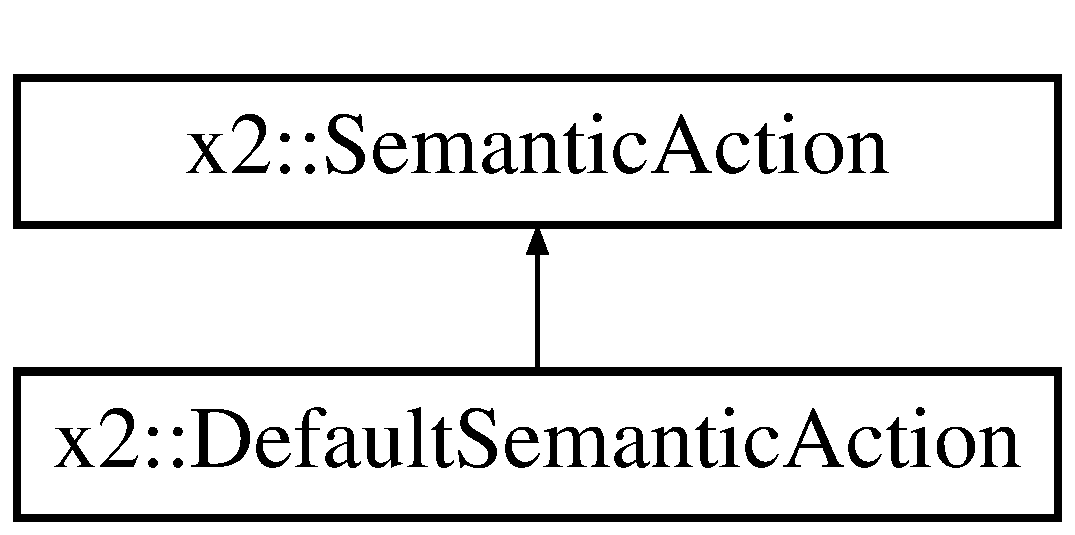
\includegraphics[height=2.000000cm]{classx2_1_1_semantic_action}
\end{center}
\end{figure}
\subsection*{Public Member Functions}
\begin{DoxyCompactItemize}
\item 
virtual void \hyperlink{classx2_1_1_semantic_action_a859c5de657a2c684fef66e04a324e980}{on\+Reduce} (int i, int j)=0
\item 
virtual void \hyperlink{classx2_1_1_semantic_action_a00d94c579c5962c74ccd5ee6bc9ef70c}{on\+No\+Goto\+Error} ()=0
\item 
virtual void \hyperlink{classx2_1_1_semantic_action_ac8afb7342d18d7d633c234047b16fe27}{on\+No\+Action\+Error} ()=0
\end{DoxyCompactItemize}


\subsection{Detailed Description}
语义动作(也就是语义规则) 使用者应当根据自己的需求来实现on\+Reduce方法 

\subsection{Member Function Documentation}
\mbox{\Hypertarget{classx2_1_1_semantic_action_ac8afb7342d18d7d633c234047b16fe27}\label{classx2_1_1_semantic_action_ac8afb7342d18d7d633c234047b16fe27}} 
\index{x2\+::\+Semantic\+Action@{x2\+::\+Semantic\+Action}!on\+No\+Action\+Error@{on\+No\+Action\+Error}}
\index{on\+No\+Action\+Error@{on\+No\+Action\+Error}!x2\+::\+Semantic\+Action@{x2\+::\+Semantic\+Action}}
\subsubsection{\texorpdfstring{on\+No\+Action\+Error()}{onNoActionError()}}
{\footnotesize\ttfamily virtual void x2\+::\+Semantic\+Action\+::on\+No\+Action\+Error (\begin{DoxyParamCaption}{ }\end{DoxyParamCaption})\hspace{0.3cm}{\ttfamily [pure virtual]}}

在\+Action\mbox{[}state,a\mbox{]}没有对应的转移的时候调用 

Implemented in \hyperlink{classx2_1_1_default_semantic_action_a6485fcbff1d9b9d63d40112d8887790d}{x2\+::\+Default\+Semantic\+Action}.

\mbox{\Hypertarget{classx2_1_1_semantic_action_a00d94c579c5962c74ccd5ee6bc9ef70c}\label{classx2_1_1_semantic_action_a00d94c579c5962c74ccd5ee6bc9ef70c}} 
\index{x2\+::\+Semantic\+Action@{x2\+::\+Semantic\+Action}!on\+No\+Goto\+Error@{on\+No\+Goto\+Error}}
\index{on\+No\+Goto\+Error@{on\+No\+Goto\+Error}!x2\+::\+Semantic\+Action@{x2\+::\+Semantic\+Action}}
\subsubsection{\texorpdfstring{on\+No\+Goto\+Error()}{onNoGotoError()}}
{\footnotesize\ttfamily virtual void x2\+::\+Semantic\+Action\+::on\+No\+Goto\+Error (\begin{DoxyParamCaption}{ }\end{DoxyParamCaption})\hspace{0.3cm}{\ttfamily [pure virtual]}}

在\+G\+O\+TO\mbox{[}state,A\mbox{]}没有对应表项的时候调用 

Implemented in \hyperlink{classx2_1_1_default_semantic_action_acbd05d5f08396b9df966494bd4422a54}{x2\+::\+Default\+Semantic\+Action}.

\mbox{\Hypertarget{classx2_1_1_semantic_action_a859c5de657a2c684fef66e04a324e980}\label{classx2_1_1_semantic_action_a859c5de657a2c684fef66e04a324e980}} 
\index{x2\+::\+Semantic\+Action@{x2\+::\+Semantic\+Action}!on\+Reduce@{on\+Reduce}}
\index{on\+Reduce@{on\+Reduce}!x2\+::\+Semantic\+Action@{x2\+::\+Semantic\+Action}}
\subsubsection{\texorpdfstring{on\+Reduce()}{onReduce()}}
{\footnotesize\ttfamily virtual void x2\+::\+Semantic\+Action\+::on\+Reduce (\begin{DoxyParamCaption}\item[{int}]{i,  }\item[{int}]{j }\end{DoxyParamCaption})\hspace{0.3cm}{\ttfamily [pure virtual]}}

在产生一个归约式的时候调用. 
\begin{DoxyParams}{Parameters}
{\em i} & \\
\hline
{\em j} & $<$i,j$>$指定使用的产生式,因为它只是个索引,所以你必须知道它所使用的文法实体 \\
\hline
\end{DoxyParams}


Implemented in \hyperlink{classx2_1_1_default_semantic_action_a25f6cc0ccc04c61ad57bfcf10b9c0cb9}{x2\+::\+Default\+Semantic\+Action}.



The documentation for this class was generated from the following file\+:\begin{DoxyCompactItemize}
\item 
D\+:/\+Pool/eclipse-\/workspace/compiler-\/debug/include/Grammar\+Translate\+Utils.\+h\end{DoxyCompactItemize}

\hypertarget{classx2_1_1_s_s_d_translator}{}\section{x2\+:\+:S\+S\+D\+Translator Class Reference}
\label{classx2_1_1_s_s_d_translator}\index{x2\+::\+S\+S\+D\+Translator@{x2\+::\+S\+S\+D\+Translator}}


{\ttfamily \#include $<$Grammar\+Translate\+Utils.\+h$>$}



\subsection{Detailed Description}
语法制导的翻译 S\+SD 产生式需要与另一个规则相互连接起来,构成\+S\+S\+D的语义规则 

The documentation for this class was generated from the following files\+:\begin{DoxyCompactItemize}
\item 
D\+:/\+Pool/eclipse-\/workspace/compiler-\/debug/include/Grammar\+Translate\+Utils.\+h\item 
D\+:/\+Pool/eclipse-\/workspace/compiler-\/debug/src/Grammar\+Translate\+Utils.\+cpp\end{DoxyCompactItemize}

\hypertarget{classx2_1_1_stream_convertor}{}\section{x2\+:\+:Stream\+Convertor Class Reference}
\label{classx2_1_1_stream_convertor}\index{x2\+::\+Stream\+Convertor@{x2\+::\+Stream\+Convertor}}


A convert word stream, it converts any input type to integer(int)  




{\ttfamily \#include $<$Lexical\+Parser.\+h$>$}

Inheritance diagram for x2\+:\+:Stream\+Convertor\+:\begin{figure}[H]
\begin{center}
\leavevmode
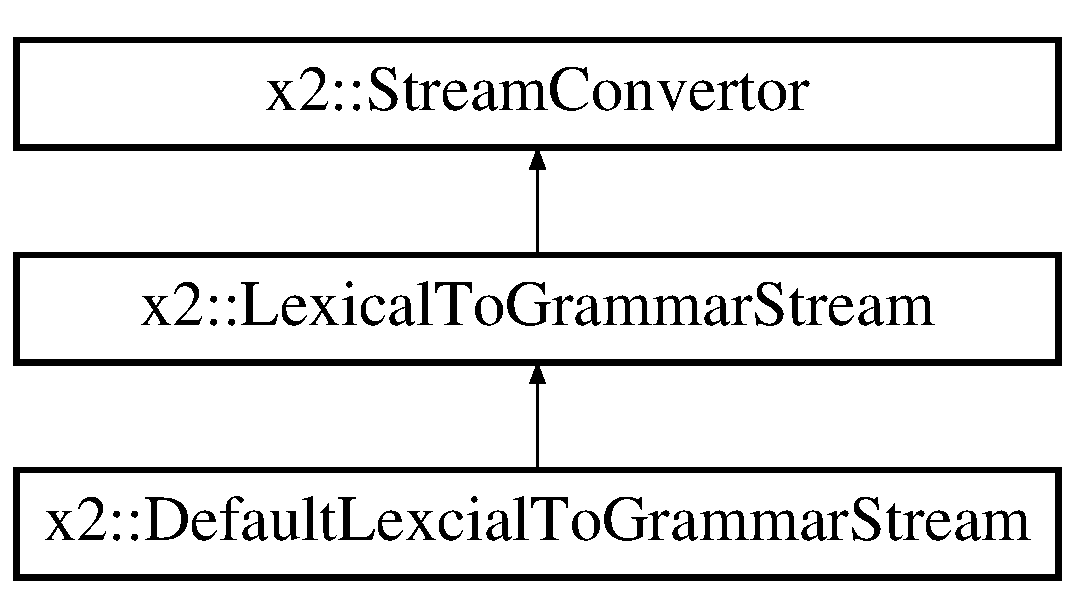
\includegraphics[height=3.000000cm]{classx2_1_1_stream_convertor}
\end{center}
\end{figure}
\subsection*{Public Types}
\begin{DoxyCompactItemize}
\item 
\mbox{\Hypertarget{classx2_1_1_stream_convertor_a1aad435b98906735d193f2dddaafcbde}\label{classx2_1_1_stream_convertor_a1aad435b98906735d193f2dddaafcbde}} 
typedef std\+::vector$<$ std\+::pair$<$ std\+::string, int $>$ $>$ {\bfseries Word\+Stream}
\end{DoxyCompactItemize}
\subsection*{Public Member Functions}
\begin{DoxyCompactItemize}
\item 
\mbox{\Hypertarget{classx2_1_1_stream_convertor_a876b8e8c24be22071be077131d630653}\label{classx2_1_1_stream_convertor_a876b8e8c24be22071be077131d630653}} 
virtual void {\bfseries go\+Backward} ()
\item 
\mbox{\Hypertarget{classx2_1_1_stream_convertor_a139c6530279fa6c4539aec126e8d18a5}\label{classx2_1_1_stream_convertor_a139c6530279fa6c4539aec126e8d18a5}} 
virtual void {\bfseries go\+Forward} ()
\item 
\mbox{\Hypertarget{classx2_1_1_stream_convertor_a5496244c269c2c59aaa8b596bf4e6e93}\label{classx2_1_1_stream_convertor_a5496244c269c2c59aaa8b596bf4e6e93}} 
virtual void {\bfseries move} (int i)=0
\item 
\mbox{\Hypertarget{classx2_1_1_stream_convertor_ad6e8220fe474334d95d0361f7bd301c4}\label{classx2_1_1_stream_convertor_ad6e8220fe474334d95d0361f7bd301c4}} 
virtual void {\bfseries go\+Head} ()=0
\item 
\mbox{\Hypertarget{classx2_1_1_stream_convertor_ab2a5c8c756da383dac62ef7e5ba15953}\label{classx2_1_1_stream_convertor_ab2a5c8c756da383dac62ef7e5ba15953}} 
virtual void {\bfseries go\+End} ()=0
\item 
virtual \hyperlink{classx2_1_1_stream_convertor}{Stream\+Convertor} \& \hyperlink{classx2_1_1_stream_convertor_a5b387cc560794db5ac2f0c35dd4023d1}{operator$>$$>$} (int \&i)=0
\item 
virtual int \hyperlink{classx2_1_1_stream_convertor_a9bc76cb1b81f1b11c9967f37f01bf2be}{peek} () const =0
\item 
virtual int \hyperlink{classx2_1_1_stream_convertor_a1025f8d8b1b1e430a6476d74e2506b10}{get} ()=0
\item 
virtual bool \hyperlink{classx2_1_1_stream_convertor_a64febc08c310555497ca497df583b940}{eof} () const =0
\end{DoxyCompactItemize}


\subsection{Detailed Description}
A convert word stream, it converts any input type to integer(int) 

a stream is an ordered input sequence, which can move backward or move forward randomly. the stream is not consumed,so it can be repeatly traversed.

It cannot be put,but only be taken. 

\subsection{Member Function Documentation}
\mbox{\Hypertarget{classx2_1_1_stream_convertor_a64febc08c310555497ca497df583b940}\label{classx2_1_1_stream_convertor_a64febc08c310555497ca497df583b940}} 
\index{x2\+::\+Stream\+Convertor@{x2\+::\+Stream\+Convertor}!eof@{eof}}
\index{eof@{eof}!x2\+::\+Stream\+Convertor@{x2\+::\+Stream\+Convertor}}
\subsubsection{\texorpdfstring{eof()}{eof()}}
{\footnotesize\ttfamily virtual bool x2\+::\+Stream\+Convertor\+::eof (\begin{DoxyParamCaption}{ }\end{DoxyParamCaption}) const\hspace{0.3cm}{\ttfamily [pure virtual]}}

judge if the stream is coming its ending 

Implemented in \hyperlink{classx2_1_1_lexical_to_grammar_stream_a813ec919763970d4150f35cba4da1db1}{x2\+::\+Lexical\+To\+Grammar\+Stream}.

\mbox{\Hypertarget{classx2_1_1_stream_convertor_a1025f8d8b1b1e430a6476d74e2506b10}\label{classx2_1_1_stream_convertor_a1025f8d8b1b1e430a6476d74e2506b10}} 
\index{x2\+::\+Stream\+Convertor@{x2\+::\+Stream\+Convertor}!get@{get}}
\index{get@{get}!x2\+::\+Stream\+Convertor@{x2\+::\+Stream\+Convertor}}
\subsubsection{\texorpdfstring{get()}{get()}}
{\footnotesize\ttfamily virtual int x2\+::\+Stream\+Convertor\+::get (\begin{DoxyParamCaption}{ }\end{DoxyParamCaption})\hspace{0.3cm}{\ttfamily [pure virtual]}}

same with operator$>$$>$ 

Implemented in \hyperlink{classx2_1_1_lexical_to_grammar_stream_a8ae8e1b6ada26785c70db1255daca798}{x2\+::\+Lexical\+To\+Grammar\+Stream}.

\mbox{\Hypertarget{classx2_1_1_stream_convertor_a5b387cc560794db5ac2f0c35dd4023d1}\label{classx2_1_1_stream_convertor_a5b387cc560794db5ac2f0c35dd4023d1}} 
\index{x2\+::\+Stream\+Convertor@{x2\+::\+Stream\+Convertor}!operator$>$$>$@{operator$>$$>$}}
\index{operator$>$$>$@{operator$>$$>$}!x2\+::\+Stream\+Convertor@{x2\+::\+Stream\+Convertor}}
\subsubsection{\texorpdfstring{operator$>$$>$()}{operator>>()}}
{\footnotesize\ttfamily virtual \hyperlink{classx2_1_1_stream_convertor}{Stream\+Convertor}\& x2\+::\+Stream\+Convertor\+::operator$>$$>$ (\begin{DoxyParamCaption}\item[{int \&}]{i }\end{DoxyParamCaption})\hspace{0.3cm}{\ttfamily [pure virtual]}}

get an input stream 

Implemented in \hyperlink{classx2_1_1_lexical_to_grammar_stream_a7b3d4b7bfc44a17905bae8dc8dcf7a40}{x2\+::\+Lexical\+To\+Grammar\+Stream}.

\mbox{\Hypertarget{classx2_1_1_stream_convertor_a9bc76cb1b81f1b11c9967f37f01bf2be}\label{classx2_1_1_stream_convertor_a9bc76cb1b81f1b11c9967f37f01bf2be}} 
\index{x2\+::\+Stream\+Convertor@{x2\+::\+Stream\+Convertor}!peek@{peek}}
\index{peek@{peek}!x2\+::\+Stream\+Convertor@{x2\+::\+Stream\+Convertor}}
\subsubsection{\texorpdfstring{peek()}{peek()}}
{\footnotesize\ttfamily virtual int x2\+::\+Stream\+Convertor\+::peek (\begin{DoxyParamCaption}{ }\end{DoxyParamCaption}) const\hspace{0.3cm}{\ttfamily [pure virtual]}}

get an input, but do not move the stream 

Implemented in \hyperlink{classx2_1_1_lexical_to_grammar_stream_a67a0e2b6ed998fd1dea1c9829be4461f}{x2\+::\+Lexical\+To\+Grammar\+Stream}.



The documentation for this class was generated from the following file\+:\begin{DoxyCompactItemize}
\item 
D\+:/\+Pool/eclipse-\/workspace/compiler-\/debug/include/Lexical\+Parser.\+h\end{DoxyCompactItemize}

%--- End generated contents ---

% Index
\backmatter
\newpage
\phantomsection
\clearemptydoublepage
\addcontentsline{toc}{chapter}{Index}
\printindex

\end{document}
